\documentclass[conference]{IEEEtran}
\usepackage{cite}
\usepackage{amsmath,amssymb,amsfonts}
\usepackage{algorithmic}
\usepackage{algorithm}
\usepackage{graphicx}
\usepackage{textcomp}
\usepackage{xcolor}
\usepackage{listings}
\usepackage{tikz}
\usepackage[hidelinks]{hyperref}
\usepackage{pgfplots}
\pgfplotsset{compat=1.18}
\usetikzlibrary{shapes.geometric, shapes.multipart, arrows.meta, positioning, calc, fit, backgrounds, shadows, decorations.pathreplacing, matrix, patterns}

% Color Definitions for Architecture Diagram
\definecolor{host_bg}{RGB}{255,250,230}
\definecolor{host_border}{RGB}{200,150,50}
\definecolor{l1_bg}{RGB}{230,240,255}
\definecolor{l1_border}{RGB}{50,100,200}
\definecolor{l1_inner_bg}{RGB}{245,250,255}
\definecolor{l2_bg}{RGB}{230,255,230}
\definecolor{l2_border}{RGB}{50,150,50}
\definecolor{l2_inner_bg}{RGB}{245,255,245}
\definecolor{l3_bg}{RGB}{255,230,230}
\definecolor{l3_border}{RGB}{200,50,50}
\definecolor{l3_inner_bg}{RGB}{255,245,245}
\definecolor{bus_color}{RGB}{80,80,80}
\definecolor{warp_text}{RGB}{100,0,100}

% Syntax Highlighting for Micro-CUDA Assembly
\lstdefinelanguage{MicroCUDA}{
  keywords={LDL, STL, IADD, IMUL, MOV, EXIT, BAR.SYNC, BRA, S2R, STX, LDX, LDG, STG, LDS, FADD, FSUB, FMUL, FFMA, SFU, ISETP, BR},
  keywordstyle=\color{blue}\bfseries,
  ndkeywords={R0, R1, R2, R3, R10, R11, R12, R20, R21, R31, F0, F1, P0, P1, SR_LANEID, SR_TID},
  ndkeywordstyle=\color{purple}\bfseries,
  identifierstyle=\color{black},
  sensitive=false,
  comment=[l]{;},
  commentstyle=\color{gray}\ttfamily,
  stringstyle=\color{red}\ttfamily,
  morestring=[b]',
  morestring=[b]"
}

\lstset{
  basicstyle=\ttfamily\footnotesize,
  language=MicroCUDA,
  frame=single,
  numbers=left,
  numberstyle=\tiny\color{gray},
  captionpos=b,
  breaklines=true
}

\def\BibTeX{{\rm B\kern-.05em{\sc i\kern-.025em b}\kern-.08em
    T\kern-.1667em\lower.7ex\hbox{E}\kern-.125emX}}

\begin{document}

\title{Micro-CUDA: A SIMT Architecture Implementation on ESP32 Dual-Core System}

\author{\IEEEauthorblockN{Hung-Wei Machine}
\IEEEauthorblockA{\textit{Department of Antigravity Engineering} \\
\textit{Deepmind Research}\\
Taipei, Taiwan \\
agent@deepmind.com}
}

\maketitle
\tableofcontents

\begin{abstract}
The proliferation of AIoT devices has created a demand for parallel computing capabilities on resource-constrained microcontrollers. However, standard MCUs lack the Single Instruction Multiple Thread (SIMT) architecture found in GPUs, limiting their efficiency in data-parallel tasks like Transformer attention mechanisms. This paper presents \textit{Micro-CUDA}, a software-defined GPU architecture implemented on the ESP32 dual-core SoC. By dedicating Core 0 to instruction scheduling (Front-End) and Core 1 to an 8-lane SIMD execution engine (Back-End), we achieve a functional SIMT pipeline with independent register files and predicated execution. We introduce Micro-CUDA ISA v1.5, which features lane-aware memory operations, enabling true data parallelism. A case study on parallel Self-Attention computation demonstrates the architecture's ability to execute GPU-like kernels, effectively bridging the gap between MCU and GPU programming models for educational and edge-computing applications.
\end{abstract}

\begin{IEEEkeywords}
ESP32, GPGPU, SIMT, Soft-GPU, Edge AI, CUDA
\end{IEEEkeywords}

\section*{Revision History}

\begin{table}[h]
\centering
\begin{tabular}{|l|l|l|p{4cm}|}
\hline
\textbf{Version} & \textbf{Date} & \textbf{Author} & \textbf{Description} \\ \hline
0.1 & 2024-10-01 & Hung-Wei Machine & Initial Draft \\ \hline
0.5 & 2024-11-15 & Hung-Wei Machine & Added Architecture \& Pipeline \\ \hline
0.9 & 2024-12-10 & Hung-Wei Machine & Added Micro-CUDA ISA \\ \hline
1.0 & 2025-12-16 & Agent & Formal Engineering Specification Release (Added Electrical Specs, ABI, Benchmarks) \\ \hline
\end{tabular}
\end{table}

\section*{Glossary}
\begin{itemize}
    \item \textbf{SMSP}: Streaming Multiprocessor Sub-Partition. The fundamental execution unit containing one SIMD core.
    \item \textbf{G-BUS}: Global Bus. 8-bit parallel bus connecting the Host (ESP32) and Device (RP2040) nodes.
    \item \textbf{Micro-CUDA}: A subset of CUDA PTX ISA adapted for microcontroller constraints.
    \item \textbf{Warp}: A group of 8 threads executed in lock-step.
\end{itemize}

\section{Introduction}
As Deep Learning models like Transformers move to the edge, the need for efficient matrix operations on embedded devices grows. While high-end edge GPUs (e.g., NVIDIA Jetson) exist, there is a significant gap in enabling GPU-like programming models on ubiquitous, low-cost microcontrollers like the ESP32.

Traditional Microcontroller Units (MCUs) operate on a SISD (Single Instruction Single Data) model. Emulating a GPU requires a fundamental architectural shift to SIMT (Single Instruction Multiple Threads). This paper proposes a novel approach to emulate a Streaming Multiprocessor (SM) using the asymmetric dual-core architecture of the ESP32.

Our contributions are as follows:
\begin{enumerate}
    \item \textbf{Dual-Core Split Architecture}: We decouple control logic (Core 0) from execution logic (Core 1) to mimic the GPU Front-End/Back-End split, utilizing FreeRTOS queues for synchronization.
    \item \textbf{Micro-CUDA ISA v1.5}: We introduce a custom 32-bit instruction set supporting predicated execution, warp synchronization, and lane-based addressing, specifically designed for MCU constraints.
    \item \textbf{Virtual SIMD Engine}: A runtime environment on Core 1 that manages 8 virtual "lanes" with isolated register contexts, enabling true data parallelism.
\end{enumerate}


% II. System Architecture
\section{System Architecture}

The system architecture defines a strict hierarchical topology, designed to physically emulate the CUDA execution model. Data flows from the high-level software abstraction on the host down to bit-level arithmetic operations in the distributed cores. The complete topological view is illustrated in Figure \ref{fig:full_architecture}.

% ==========================================
% TikZ Architecture Diagram
% ==========================================
\begin{figure*} % figure* 讓圖表橫跨兩欄
    \centering
    % 使用 resizebox 自動將圖縮放至頁面寬度 (\textwidth)
    \resizebox{0.95\textwidth}{!}{%
    
    % --- 開始你的 TikZ 程式碼 ---
    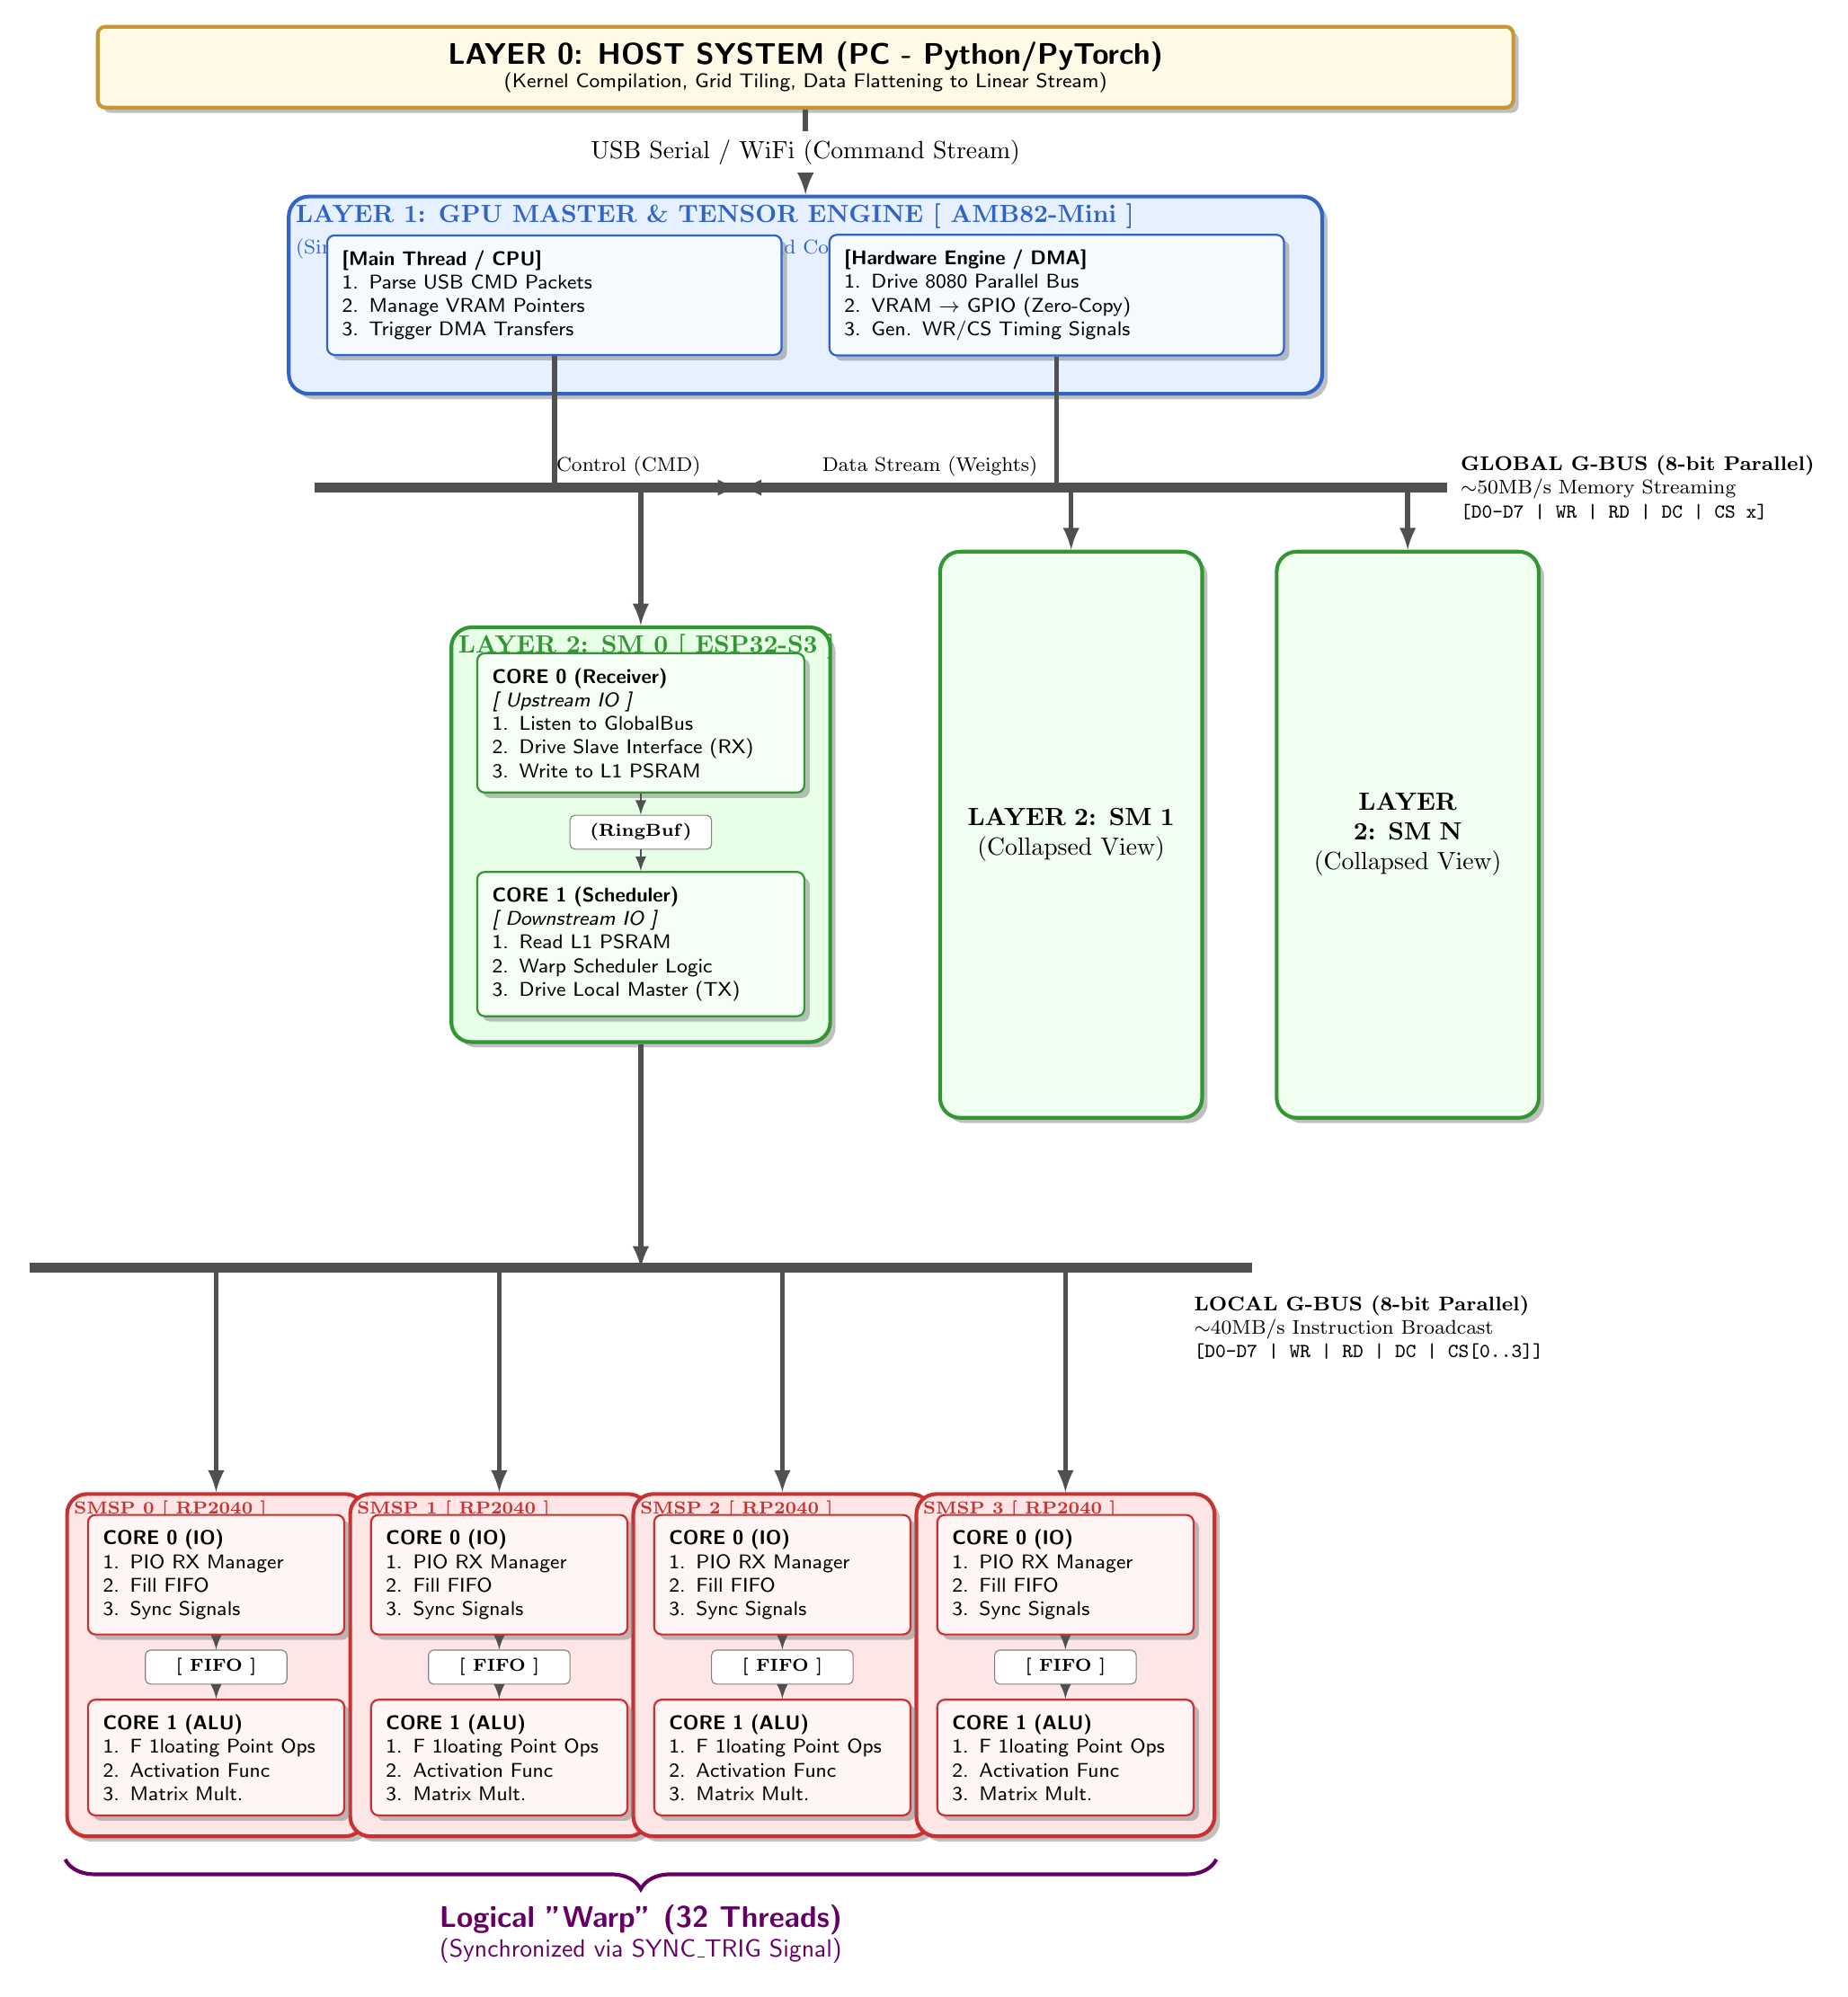
\begin{tikzpicture}[
        node distance=1.5cm, 
        % --- Styles ---
        base_box/.style={
            rectangle, draw, rounded corners=3pt, align=left, drop shadow,
            font=\sffamily\footnotesize, inner sep=6pt
        },
        % Layer Containers
        host_box/.style={base_box, draw=host_border, fill=host_bg, line width=1.5pt, align=center},
        l1_cont/.style={draw=l1_border, fill=l1_bg, rounded corners=8pt, line width=1.5pt, inner sep=15pt, drop shadow},
        l2_cont/.style={draw=l2_border, fill=l2_bg, rounded corners=8pt, line width=1.5pt, inner sep=10pt, drop shadow},
        l3_cont/.style={draw=l3_border, fill=l3_bg, rounded corners=8pt, line width=1.5pt, inner sep=8pt, drop shadow},
        % Internal Modules (White/Light boxes)
        l1_node/.style={base_box, draw=l1_border, fill=l1_inner_bg, text width=6.0cm, line width=0.8pt},
        l2_node/.style={base_box, draw=l2_border, fill=l2_inner_bg, text width=4.2cm, line width=0.8pt},
        l3_node/.style={base_box, draw=l3_border, fill=l3_inner_bg, text width=3.2cm, line width=0.8pt},
        fifo_node/.style={rectangle, draw=gray, fill=white, rounded corners=2pt, font=\scriptsize\bfseries, align=center, minimum width=2cm},
        % Lines
        bus_line/.style={draw=bus_color, line width=2pt, -latex},
        thin_line/.style={draw=bus_color, line width=1pt, -latex},
        % Style for the underbrace
        warp_brace/.style={decorate, decoration={brace, amplitude=12pt, mirror}, line width=1.5pt, draw=warp_text}
    ]

    % =========================================================================
    % LAYER 0: HOST SYSTEM
    % =========================================================================
    \node[host_box, minimum width=20cm] (host) {
        \textbf{\large LAYER 0: HOST SYSTEM (PC - Python/PyTorch)}\\
        (Kernel Compilation, Grid Tiling, Data Flattening to Linear Stream)
    };

    % =========================================================================
    % LAYER 1: AMB82-Mini (Dual Logic)
    % =========================================================================
    \node[below=2.5cm of host] (l1_center_helper) {};

    \node[l1_node, left=0.2cm of l1_center_helper] (l1_cpu) {
        \textbf{[Main Thread / CPU]}\\
        1. Parse USB CMD Packets\\
        2. Manage VRAM Pointers\\
        3. Trigger DMA Transfers
    };
    
    \node[l1_node, right=0.2cm of l1_center_helper] (l1_dma) {
        \textbf{[Hardware Engine / DMA]}\\
        1. Drive 8080 Parallel Bus\\
        2. VRAM $\to$ GPIO (Zero-Copy)\\
        3. Gen. WR/CS Timing Signals
    };

    \begin{scope}[on background layer]
        \node[l1_cont, fit=(l1_cpu)(l1_dma)] (l1_container) {};
        \node[anchor=north west, text=l1_border, font=\bfseries] at (l1_container.north west) {LAYER 1: GPU MASTER \& TENSOR ENGINE [ AMB82-Mini ]};
        \node[anchor=north west, text=l1_border, font=\footnotesize] at ($(l1_container.north west)+(0,-0.5)$) {(Single-core M33, utilizing DMA HW as a virtual 2nd Core)};
    \end{scope}

    \draw[bus_line] (host.south) -- node[midway, fill=white] {USB Serial / WiFi (Command Stream)} (l1_container.north);

    % =========================================================================
    % LAYER 2: ESP32-S3 (Dual Core Vertical)
    % =========================================================================
    \node[below=4.5cm of l1_container.south west, xshift=5cm] (sm0_center) {};

    \node[l2_node] (sm0_core0) at (sm0_center) {
        \textbf{CORE 0 (Receiver)}\\
        \textit{[ Upstream IO ]}\\
        1. Listen to GlobalBus\\
        2. Drive Slave Interface (RX)\\
        3. Write to L1 PSRAM
    };
    
    \node[fifo_node, below=0.3cm of sm0_core0] (sm0_ring) {(RingBuf)};
    
    \node[l2_node, below=0.3cm of sm0_ring] (sm0_core1) {
        \textbf{CORE 1 (Scheduler)}\\
        \textit{[ Downstream IO ]}\\
        1. Read L1 PSRAM\\
        2. Warp Scheduler Logic\\
        3. Drive Local Master (TX)
    };

    \begin{scope}[on background layer]
        \node[l2_cont, fit=(sm0_core0)(sm0_ring)(sm0_core1)] (sm0_container) {};
        \node[anchor=north west, text=l2_border, font=\bfseries] at (sm0_container.north west) {LAYER 2: SM 0 [ ESP32-S3 ]};
    \end{scope}

    \draw[thin_line] (sm0_core0) -- (sm0_ring);
    \draw[thin_line] (sm0_ring) -- (sm0_core1);

    % --- SM 1 & SM N (Collapsed) ---
    \node[l2_cont, right=1.5cm of sm0_container, minimum height=8cm, text width=3cm, align=center, fill=l2_bg!60] (sm1_container) {
        \textbf{LAYER 2: SM 1}\\(Collapsed View)
    };
    \node[l2_cont, right=1.0cm of sm1_container, minimum height=8cm, text width=3cm, align=center, fill=l2_bg!60] (smn_container) {
        \textbf{LAYER 2: SM N}\\(Collapsed View)
    };

    % =========================================================================
    % GLOBAL BUS (L1 -> L2)
    % =========================================================================
    \coordinate (gbus_y) at ($(l1_container.south)!0.4!(sm0_container.north)$);
    
    \draw[bus_line] (l1_cpu.south) |- (gbus_y) node[pos=0.7, above, font=\footnotesize] {Control (CMD)};
    \draw[bus_line] (l1_dma.south) |- (gbus_y) node[pos=0.7, above, font=\footnotesize] {Data Stream (Weights)};
    
    \draw[line width=4pt, draw=bus_color] ($(gbus_y) + (-6,0)$) -- ($(gbus_y) + (10,0)$) 
        node[right, align=left, font=\footnotesize] {
            \textbf{GLOBAL G-BUS (8-bit Parallel)}\\
            $\sim$50MB/s Memory Streaming\\
            \texttt{[D0-D7 | WR | RD | DC | CS x]}
        };
    
    \draw[bus_line] (gbus_y -| sm0_container.north) -- (sm0_container.north);
    \draw[bus_line] (gbus_y -| sm1_container.north) -- (sm1_container.north);
    \draw[bus_line] (gbus_y -| smn_container.north) -- (smn_container.north);

    % =========================================================================
    % LAYER 3: RP2040 (Dual Core Vertical)
    % =========================================================================
    
    % Macro for drawing SMSP
    \newcommand{\drawSMSP}[3]{
        \node[l3_node] (#1_core0) at (#2) {
            \textbf{CORE 0 (IO)}\\
            1. PIO RX Manager\\
            2. Fill FIFO\\
            3. Sync Signals
        };
        \node[fifo_node, below=0.2cm of #1_core0] (#1_fifo) {[ FIFO ]};
        \node[l3_node, below=0.2cm of #1_fifo] (#1_core1) {
            \textbf{CORE 1 (ALU)}\\
            1. F 1loating Point Ops\\
            2. Activation Func\\
            3. Matrix Mult.
        };
        
        \begin{scope}[on background layer]
            \node[l3_cont, fit=(#1_core0)(#1_fifo)(#1_core1)] (#1_cont) {};
            \node[anchor=north west, text=l3_border, font=\bfseries\scriptsize] at (#1_cont.north west) {#3};
        \end{scope}
        
        \draw[thin_line] (#1_core0) -- (#1_fifo);
        \draw[thin_line] (#1_fifo) -- (#1_core1);
    }

    \coordinate (l3_start_y) at ($(sm0_container.south) + (0, -7.5cm)$);
    
    \drawSMSP{smsp0}{$(l3_start_y) + (-6.0, 0)$}{SMSP 0 [ RP2040 ]}
    \drawSMSP{smsp1}{$(l3_start_y) + (-2.0, 0)$}{SMSP 1 [ RP2040 ]}
    \drawSMSP{smsp2}{$(l3_start_y) + ( 2.0, 0)$}{SMSP 2 [ RP2040 ]}
    \drawSMSP{smsp3}{$(l3_start_y) + ( 6.0, 0)$}{SMSP 3 [ RP2040 ]}

    % =========================================================================
    % LOCAL BUS (L2 -> L3)
    % =========================================================================
    \coordinate (lbus_y) at ($(sm0_container.south)!0.5!(smsp0_cont.north)$);
    
    \draw[bus_line] (sm0_container.south) -- (lbus_y -| sm0_container.south);
    
    \draw[line width=4pt, draw=bus_color] ($(lbus_y -| smsp0_cont.west) + (-0.5,0)$) -- ($(lbus_y -| smsp3_cont.east) + (0.5,0)$) 
        node[below right, align=left, font=\footnotesize, xshift=-1cm, yshift=-0.2cm] {
            \textbf{LOCAL G-BUS (8-bit Parallel)}\\
            $\sim$40MB/s Instruction Broadcast\\
            \texttt{[D0-D7 | WR | RD | DC | CS[0..3]]}
        };
    
    \foreach \i in {0,1,2,3} {
        \draw[bus_line] (lbus_y -| smsp\i_cont.north) -- (smsp\i_cont.north);
    }

    % =========================================================================
    % Warp Brace
    % =========================================================================
    \coordinate (brace_start) at ($(smsp0_cont.south west) + (0, -0.3cm)$);
    \coordinate (brace_end) at ($(smsp3_cont.south east) + (0, -0.3cm)$);

    \draw[warp_brace] (brace_start) -- (brace_end)
        node[midway, below=0.5cm, align=center, font=\sffamily, text=warp_text] {
            \textbf{\large Logical "Warp" (32 Threads)}\\
            (Synchronized via SYNC\_TRIG Signal)
        };

    \end{tikzpicture}
    % --- 結束 TikZ 程式碼 ---
SP32-S3 as Streamin    } % 結束 resizebox
    \caption{Detailed System Architecture. The hierarchy moves from the Host (Grid) to the AMB82-Mini (Controller), then to ESP32-S3s (Streaming Multiprocessors), and finally to RP2040s (Threads).}
    \label{fig:full_architecture}
\end{figure*}

\subsection{Cluster Hierarchy}

\subsubsection{Layer 0: Host System (Grid)}
The host PC utilizes PyTorch to define the computational graph. It performs \textbf{Grid Tiling}, breaking large tensors into smaller chunks that fit the SRAM constraints of the microcontroller network. These tiles are flattened into a serial stream.

\subsubsection{Layer 1: GPU Master (AMB82-Mini)}
This layer acts as the centralized controller. It features an ARM Cortex-M33 core.
\begin{itemize}
    \item \textbf{DMA Engine:} The defining feature is the use of the DMA hardware as a "Virtual Second Core." It drives the 8080 parallel bus, generating Write (WR) and Chip Select (CS) signals automatically.
\end{itemize}

\subsubsection{Layer 2: Streaming Multiprocessors (ESP32-S3)}
The ESP32-S3 mimics a CUDA SM. It utilizes its dual-core architecture to decouple reception from scheduling. Core 0 fills a Ring Buffer from the Global Bus, while Core 1 reads from this buffer to schedule instructions for the downstream threads.

\subsubsection{Layer 3: SMSP / Threads (RP2040)}
The RP2040 acts as the fundamental ALU. It uses its Programmable I/O (PIO) state machines to ingest instructions from the Local G-Bus, pushing them into a FIFO for executing.

\subsection{ESP32-S3 Micro-Architecture (Node Detail)}

While the global architecture describes the cluster data flow, the specific implementation of the "Micro-CUDA" VM on the ESP32-S3 node mimics a discrete GPU's internal structure. Figure \ref{fig:vm_arch} illustrates the internal dual-core topology corresponding to the system architecture described in the ISA guide.

\begin{figure*}[htbp]
    \centering
    \resizebox{0.9\textwidth}{!}{%
    \begin{tikzpicture}[
        node distance=1.2cm,
        box/.style={rectangle, draw=black, thick, rounded corners, align=center, font=\sffamily\small},
        core_box/.style={rectangle, draw=black, line width=1pt, rounded corners, inner sep=10pt, align=center},
        mem_box/.style={rectangle, draw=black, thick, fill=yellow!10, minimum width=3cm, minimum height=1cm, align=center},
        queue_box/.style={rectangle, draw=purple, thick, dashed, fill=purple!5, minimum width=4cm, minimum height=0.8cm, align=center},
        arrow/.style={->, >=stealth, thick}
    ]

    % --- Host Node ---
    \node[box, fill=gray!20, minimum width=10cm] (host) {\textbf{HOST (Serial CLI)}\\Commands: \texttt{gpu\_reset}, \texttt{load\_imem}, \texttt{dma\_h2d}, \texttt{kernel\_launch}};

    % --- Core 0 (Front-End) ---
    \node[core_box, fill=blue!5, below=1.5cm of host, xshift=-4cm] (core0) {
        \textbf{Core 0: Front-End (Warp Scheduler)} \\[0.2cm]
        
        \begin{tikzpicture}[node distance=0.8cm]
            \node[box, fill=white] (cli) {[Serial Handler] $\to$ [CLI Parser]};
            
            \node[mem_box, below=0.5cm of cli] (imem) {
                \textbf{Instruction Memory (IMEM)}\\
                Size: 1024 Insts\\
                \scriptsize \texttt{PC:0 MOV R1,5}
            };
            
            \node[box, fill=white, below=0.5cm of imem] (fetch) {
                \textbf{Fetch \& Decode Unit}\\
                PC Control (BRA/BR.Z)\\
                Decode Opcode/Operands
            };
            
            \draw[arrow] (cli) -- (imem);
            \draw[arrow] (imem) -- (fetch);
        \end{tikzpicture}
    };

    % --- Core 1 (Back-End) ---
    \node[core_box, fill=green!5, right=1.0cm of core0] (core1) {
        \textbf{Core 1: Back-End (SIMD Engine)} \\[0.2cm]
        
        \begin{tikzpicture}[node distance=0.8cm]
            \node[box, fill=white, minimum width=5cm] (simd) {
                \textbf{8-Lane SIMD Execution Engine}\\
                \scriptsize Lane 0 .. Lane 7 (R/F/P Registers)
            };
            
            \node[mem_box, below=0.5cm of simd, fill=orange!10] (vram) {
                \textbf{Shared Global Memory (VRAM)}\\
                Size: 40KB - 1MB\\
                Shared Address Space
            };
            
            \node[box, fill=white, below=0.5cm of vram] (trace) {
                \textbf{Execution Trace Logger}\\
                Cycle-Accurate JSON Stream
            };
            
            \draw[arrow] (simd) -- (vram);
            \draw[arrow] (vram) -- (trace);
        \end{tikzpicture}
    };

    % --- Interconnects ---
    \draw[arrow, line width=1.5pt] (host) -- node[midway, fill=white] {UART (115200/Turbo)} (core0.north);
    
    % FreeRTOS Queue
    \node[queue_box, below right=0.5cm and -1cm of core0.east] (queue) {\textbf{FreeRTOS Queue}\\(Instruction Batch)};
    
    \draw[arrow, thick, blue] (core0.east) |- (queue.west);
    \draw[arrow, thick, blue] (queue.east) -| (core1.north);

    \end{tikzpicture}
    }
    \caption{ESP32-S3 Internal Micro-Architecture. Host commands drive Core 0, which fetches instructions and dispatches them via a queue to the Core 1 SIMD engine for parallel execution over shared VRAM.}
    \label{fig:vm_arch}
\end{figure*}

\begin{enumerate}
    \item \textbf{Core 0 (Warp Scheduler)}: Fetches instructions, handles PC control (Branching), and queues batches for execution.
    \item \textbf{Core 1 (SIMD Engine)}: Conceptually executes parallel lanes. Core 1 maintains 8 independent register contexts (Micro-CUDA VM mode) or drives external ALUs.
\end{enumerate}

This dual-core split allows the "SM" to maintain high throughput by overlapping instruction fetch/decode (Core 0) with mathematical execution (Core 1).

\subsection{Scalability and Multi-Chip Integration}
To scale beyond a single node, the architecture supports a hierarchical cluster topology.

\subsubsection{Inter-Node Communication}
Multiple ESP32-S3 nodes (Layer 2) are connected via a high-speed SPI bus (50 MHz) to a central master (FPGA or Gateway). This allows the host to broadcast kernels to the entire cluster or address specific nodes for task parallelism.

\subsubsection{Global Synchronization}
To support multi-chip kernels (e.g., distributed matrix multiplication), a dedicated open-drain GPIO line acts as a wired-AND "Global Barrier". When a kernel reaches a global sync point, it pulls the line low. The line only returns high when all nodes have released it, ensuring $<1\mu s$ synchronization latency across the cluster.

\subsection{Layer 1 Detail: AMB82-Mini (Master Controller)}
The AMB82-Mini serves as the high-level scheduler, implementing an Asymmetric Multi-Processing (AMP) model to manage the flow of data from the host to the distributed compute nodes.

\begin{figure*}[htbp]
\centering
\resizebox{0.95\textwidth}{!}{%
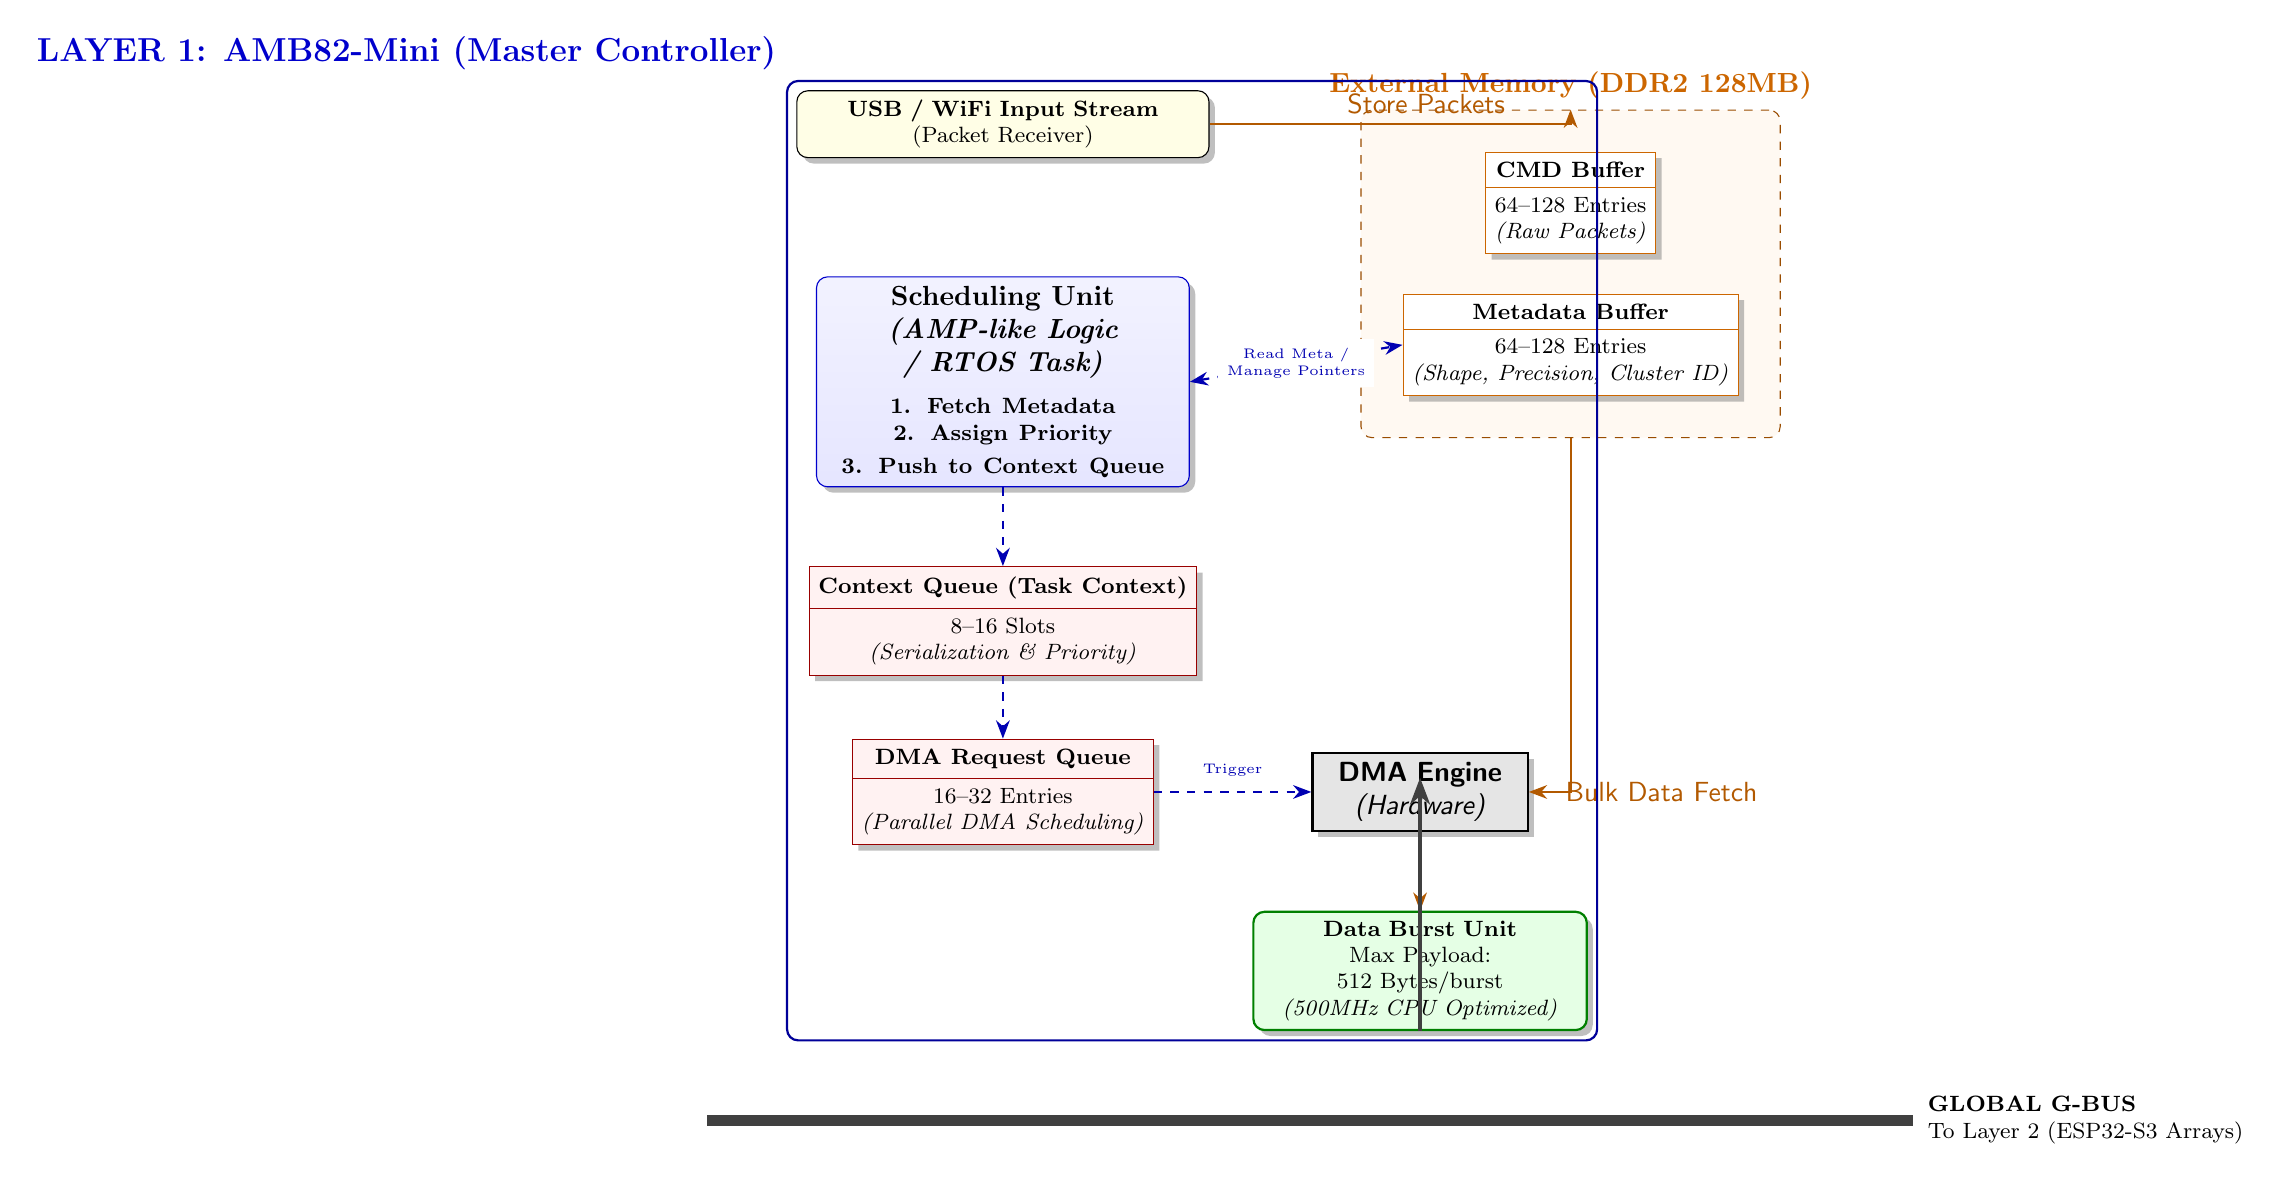
\begin{tikzpicture}[
    font=\sffamily,
    % 樣式定義
    component/.style={
        draw, fill=white, rounded corners, align=center, drop shadow, font=\footnotesize
    },
    scheduler_block/.style={
        draw=blue!80!black, top color=blue!5, bottom color=blue!10, 
        rounded corners, align=center, drop shadow, font=\bfseries
    },
    memory_container/.style={
        draw=orange!60!black, fill=orange!5, dashed, rounded corners, inner sep=15pt,
        label={[orange!80!black, font=\bfseries]north:External Memory (DDR2 128MB)}
    },
    buffer_block/.style={
        draw=orange!80!black, fill=white, rectangle split, rectangle split parts=2, 
        align=center, drop shadow, font=\footnotesize
    },
    queue_block/.style={
        draw=red!60!black, fill=red!5, rectangle split, rectangle split parts=2,
        align=center, drop shadow, font=\footnotesize, minimum width=3.5cm
    },
    dma_block/.style={
        draw=black, fill=gray!20, thick, align=center, drop shadow
    },
    bus/.style={
        draw=darkgray, line width=4pt
    },
    bus_arrow/.style={
        ->, >=Stealth, thick, color=darkgray, line width=1.5pt
    },
    control_flow/.style={
        ->, >=Stealth, dashed, blue!70!black, thick
    },
    data_flow/.style={
        ->, >=Stealth, thick, orange!70!black
    }
]

    % --- 1. TOP INTERFACE (Host Input) ---
    \node[component, fill=yellow!10, text width=5cm] (host_io) at (0, 0) {
        \textbf{USB / WiFi Input Stream}\\
        (Packet Receiver)
    };

    % --- 2. DDR2 MEMORY BLOCK (Right Side) ---
    % Increased spacing from 2cm to 3.5cm to prevent overlap
    \node[buffer_block, right=3.5cm of host_io, yshift=-1cm] (ddr_buffers) {
        \textbf{CMD Buffer}
        \nodepart{second} 64--128 Entries\\
        \textit{(Raw Packets)}
    };
    
    \node[buffer_block, below=0.5cm of ddr_buffers] (meta_buffers) {
        \textbf{Metadata Buffer}
        \nodepart{second} 64--128 Entries\\
        \textit{(Shape, Precision, Cluster ID)}
    };

    \begin{scope}[on background layer]
        % Removed explicit label to avoid duplication with style definition
        \node[memory_container, fit=(ddr_buffers) (meta_buffers)] (ddr_frame) {};
    \end{scope}

    % Connect Host to DDR
    \draw[data_flow] (host_io.east) -| (ddr_frame.north) node[pos=0.3, above] {Store Packets};

    % --- 3. AMP SCHEDULER (Center) ---
    \node[scheduler_block, below=1.5cm of host_io, text width=4.5cm, minimum height=2cm] (scheduler) {
        \textbf{Scheduling Unit}\\
        \textit{(AMP-like Logic / RTOS Task)}\\
        \vspace{0.2cm}
        \footnotesize
        1. Fetch Metadata\\
        2. Assign Priority\\
        3. Push to Context Queue
    };

    % Interaction: Scheduler reads DDR
    \draw[control_flow, <->] (scheduler.east) -- node[midway, fill=white, font=\tiny, align=center] {Read Meta /\\Manage Pointers} (meta_buffers.west);

    % --- 4. QUEUING SYSTEM (Below Scheduler) ---
    
    % Context Queue
    \node[queue_block, below=1cm of scheduler] (ctx_queue) {
        \textbf{Context Queue (Task Context)}
        \nodepart{second} 8--16 Slots\\
        \textit{(Serialization \& Priority)}
    };

    % DMA Request Queue
    \node[queue_block, below=0.8cm of ctx_queue] (dma_queue) {
        \textbf{DMA Request Queue}
        \nodepart{second} 16--32 Entries\\
        \textit{(Parallel DMA Scheduling)}
    };

    % Flow: Scheduler -> Ctx -> DMA
    \draw[control_flow] (scheduler.south) -- (ctx_queue.north);
    \draw[control_flow] (ctx_queue.south) -- (dma_queue.north);

    % --- 5. EXECUTION ENGINE (Bottom) ---
    
    % DMA Engine
    % Align clearly to the right
    \node[dma_block, right=2.0cm of dma_queue, text width=2.5cm] (dma_engine) {
        \textbf{DMA Engine}\\
        \textit{(Hardware)}
    };

    % Data Burst Unit
    \node[component, below=1cm of dma_engine, text width=4cm, fill=green!10, draw=green!50!black, thick] (burst_unit) {
        \textbf{Data Burst Unit}\\
        Max Payload: 512 Bytes/burst\\
        \textit{(500MHz CPU Optimized)}
    };

    % Connecting Memory Data to Output via DMA
    % Rerouted to enter from NORTH for cleaner vertical flow
    \draw[data_flow] (ddr_frame.south) |- (dma_engine.east) node[near end, right, xshift=2pt] {Bulk Data Fetch};
    \draw[control_flow] (dma_queue.east) -- (dma_engine.west) node[midway, above, font=\tiny, yshift=2pt] {Trigger};
    \draw[data_flow] (dma_engine.south) -- (burst_unit.north);

    % --- 6. LAYER FRAME ---
    \node[draw=blue!60!black, thick, rounded corners, fit=(host_io) (scheduler) (burst_unit) (dma_queue), label={[blue!80!black, font=\large\bfseries]north west:LAYER 1: AMB82-Mini (Master Controller)}] (layer1_frame) {};

    % --- 7. GLOBAL BUS INTERFACE ---
    \draw[bus] ($(layer1_frame.south west) + (-1, -1)$) -- ($(layer1_frame.south east) + (4, -1)$) node[right, align=left, font=\footnotesize] {
        \textbf{GLOBAL G-BUS}\\
        To Layer 2 (ESP32-S3 Arrays)
    };

    \draw[bus_arrow] (burst_unit.south) -- (burst_unit.south |- layer1_frame.south |- 0, -8.3);

\end{tikzpicture}
}
\caption{Layer 1 AMP Architecture: The AMB82-Mini effectively utilizes its DMA engine as a secondary processor, managed by an AMP-like scheduler that orchestrates context switching and priorities in external DDR memory.}
\label{fig:layer1_arch}
\end{figure*}

\subsection{Layer 2 Detail: ESP32-S3 as Streaming Multiprocessor}
The ESP32-S3 functions as the critical Layer 2 \textit{Streaming Multiprocessor (SM)}, bridging the high-bandwidth Global Bus and the localized execution threads. Its detailed internal architecture is shown in Figure \ref{fig:layer2_arch}.

\begin{figure*}[htbp]
\centering
\resizebox{0.95\textwidth}{!}{%
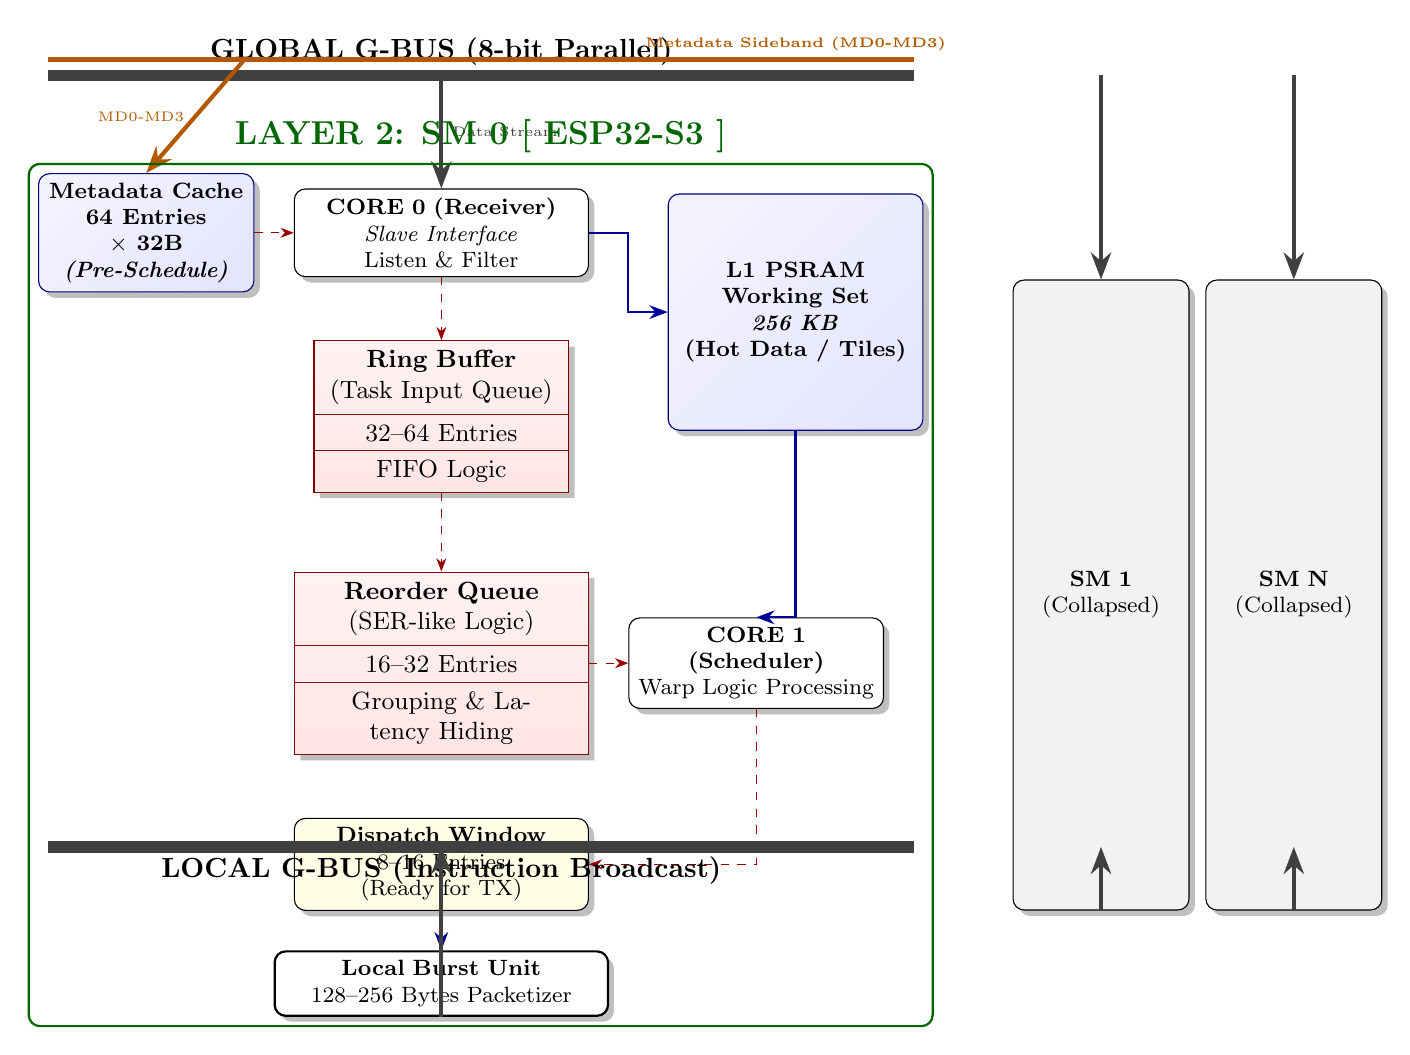
\begin{tikzpicture}[
    font=\sffamily,
    % 樣式定義
    component/.style={
        draw, fill=white, rounded corners, align=center, drop shadow, font=\footnotesize
    },
    core_block/.style={
        draw=gray, dashed, fill=gray!5, rounded corners, inner sep=10pt
    },
    memory_block/.style={
        draw=blue!50!black, top color=blue!5, bottom color=blue!10, 
        shading angle=45, rounded corners, align=center, drop shadow, font=\footnotesize\bfseries
    },
    queue_block/.style={
        draw=red!50!black, top color=red!5, bottom color=red!10, 
        rectangle split, rectangle split parts=3, align=center, drop shadow, font=\small
    },
    bus/.style={
        draw=darkgray, line width=4pt
    },
    bus_arrow/.style={
        ->, >=Stealth, thick, color=darkgray, line width=1.5pt
    },
    data_flow/.style={
        ->, >=Stealth, thick, blue!60!black
    },
    control_flow/.style={
        ->, >=Stealth, dashed, red!60!black
    }
]

    % --- 1. GLOBAL BUS (Top) ---
    \node (bus_label) at (0, 0) [above, font=\bfseries] {GLOBAL G-BUS (8-bit Parallel)};
    \draw[bus] (-5, 0) -- (6, 0);
    
    % Sideband visually separated
    \draw[bus, color=orange!70!black, line width=2pt] (-5, 0.2) -- (6, 0.2);
    \node at (4.5, 0.4) [font=\tiny\bfseries, text=orange!70!black] {Metadata Sideband (MD0-MD3)};

    % --- 2. ESP32-S3 SM 0 CONTAINER ---
    
    % --- CORE 0 AREA (Receiver) ---
    \node[component, text width=3.5cm] (rx_unit) at (0, -2) {
        \textbf{CORE 0 (Receiver)}\\
        \textit{Slave Interface}\\
        Listen \& Filter
    };

    % Metadata Cache (Sideband Processing)
    \node[memory_block, left=0.5cm of rx_unit, text width=2.5cm, fill=orange!10] (meta_cache) {
        \textbf{Metadata Cache}\\
        64 Entries $\times$ 32B\\
        \textit{(Pre-Schedule)}
    };

    % Connections from Bus
    \draw[bus_arrow, orange!70!black] (-2.5, 0.2) -- node[left, font=\tiny] {MD0-MD3} (meta_cache.north);
    \draw[bus_arrow] (0, 0) -- node[right, font=\tiny] {Data Stream} (rx_unit.north);
    \draw[control_flow] (meta_cache) -- (rx_unit);

    % --- MEMORY & BUFFERS (Middle Layer) ---
    
    % L1 PSRAM (Big Shared Pool)
    \node[memory_block, right=1cm of rx_unit, text width=3cm, minimum height=3cm, anchor=north west, yshift=0.5cm] (psram) {
        \textbf{L1 PSRAM}\\
        \textbf{Working Set}\\
        \textit{256 KB}\\
        (Hot Data / Tiles)
    };

    % Ring Buffer (Task Queue)
    \node[queue_block, below=0.8cm of rx_unit, text width=3cm] (ring_buf) {
        \textbf{Ring Buffer}\\
        (Task Input Queue)
        \nodepart{second} 32--64 Entries
        \nodepart{third} FIFO Logic
    };

    % Data write flow
    \draw[data_flow] (rx_unit.east) -- ++(0.5,0) |- (psram.west);
    \draw[control_flow] (rx_unit.south) -- (ring_buf.north);

    % --- CORE 1 AREA (Scheduler) ---
    
    % Reorder Queue
    \node[queue_block, below=1cm of ring_buf, text width=3.5cm] (reorder_q) {
        \textbf{Reorder Queue}\\
        (SER-like Logic)
        \nodepart{second} 16--32 Entries
        \nodepart{third} Grouping \& Latency Hiding
    };

    % Core 1 Logic
    \node[component, right=0.5cm of reorder_q, text width=3cm] (core1_logic) {
        \textbf{CORE 1 (Scheduler)}\\
        Warp Logic Processing
    };

    % Dispatch Window
    \node[component, below=0.8cm of reorder_q, text width=3.5cm, fill=yellow!10] (dispatch) {
        \textbf{Dispatch Window}\\
        8--16 Entries\\
        (Ready for TX)
    };

    % Burst Unit
    \node[component, below=0.5cm of dispatch, text width=4cm, draw=black, thick] (burst_unit) {
        \textbf{Local Burst Unit}\\
        128--256 Bytes Packetizer
    };

    % Core 1 Flows
    \draw[control_flow] (ring_buf.south) -- (reorder_q.north);
    \draw[data_flow] (psram.south) |- (core1_logic.north);
    \draw[control_flow] (reorder_q.east) -- (core1_logic.west);
    \draw[control_flow] (core1_logic.south) |- (dispatch.east);
    \draw[data_flow] (dispatch.south) -- (burst_unit.north);

    % --- FRAME FOR SM 0 ---
    \node[draw=green!40!black, thick, rounded corners, fit=(rx_unit) (meta_cache) (psram) (burst_unit), label={[green!40!black, font=\large\bfseries]north:LAYER 2: SM 0 [ ESP32-S3 ]}] (sm0_frame) {};

    % --- NEIGHBOR SMs (Collapsed) ---
    \node[component, right=1cm of sm0_frame, minimum height=8cm, text width=2cm, fill=gray!10] (sm1) {
        \textbf{SM 1}\\
        (Collapsed)
    };
    \node[component, right=0.2cm of sm1, minimum height=8cm, text width=2cm, fill=gray!10] (smn) {
        \textbf{SM N}\\
        (Collapsed)
    };
    
    % Bus connections for neighbors
    \draw[bus_arrow] (sm1.north |- 0,0) -- (sm1.north);
    \draw[bus_arrow] (smn.north |- 0,0) -- (smn.north);

    % --- 3. LOCAL BUS (Bottom) ---
    \coordinate (local_bus_y) at ($(burst_unit.south) + (0,-0.8)$);
    \draw[bus] (-5, -9.8) -- (6, -9.8);
    \node at (0, -10.1) [font=\bfseries] {LOCAL G-BUS (Instruction Broadcast)};

    % Output connection
    \draw[bus_arrow] (burst_unit.south) -- (0, -9.8);
    \draw[bus_arrow] (sm1.south) -- (sm1.south |- 0, -9.8);
    \draw[bus_arrow] (smn.south) -- (smn.south |- 0, -9.8);

\end{tikzpicture}
}
\caption{Layer 2 Internal Architecture: The ESP32-S3 SM Architecture showing the split between Core 0 (Receiver) and Core 1 (Scheduler), connected by ring buffers and shared L1 PSRAM.}
\label{fig:layer2_arch}
\end{figure*}

The architecture adopts a heterogeneous dual-core strategy:
\begin{itemize}
    \item \textbf{Core 0 (Receiver)}: Dedicated to high-throughput I/O. It filters incoming packets from the Global Bus based on metadata sidebands (MD0-MD3), placing valid tasks into a FIFO Ring Buffer.
    \item \textbf{Core 1 (Scheduler)}: Implements complex warp scheduling logic. It pulls tasks from the buffer, reorders them to hide memory latency (via Reorder Queue), and dispatches instruction packets to the localized worker threads via the Local G-Bus.
\end{itemize}

\subsection{Hardware Specifications}

\subsubsection{AMB82-Mini (GPU Grid Master)}
The AMB82-Mini serves as the cluster controller and edge computing node, providing the necessary computational power for coordination and AI acceleration.
\begin{itemize}
    \item \textbf{MCU}: ARMv8-M (Cortex-M33), up to 500MHz. Optimized for high-speed control and coordination tasks within the cluster.
    \item \textbf{NPU}: Intelligent Engine (0.4 TOPS). Supports efficient AI inference and accelerates edge neural networks.
    \item \textbf{Memory}: Built-in DDR2 128MB + External 16MB SPI Nor Flash. Utilized as the primary buffer for the GPU Grid and for firmware storage.
    \item \textbf{Peripherals Overview}:
    \begin{itemize}
        \item \textbf{GPIO}: Up to 23 pins.
        \item \textbf{PWM}: 8 channels.
        \item \textbf{UART}: 3 interfaces.
        \item \textbf{SPI}: 2 interfaces.
        \item \textbf{I2C}: 1 interface.
    \end{itemize}
\end{itemize}

\subsubsection{Comparison: RP2040 vs. ESP32}
Table \ref{tab:chip_comparison} provides a detailed comparison between the execution units (RP2040) and the streaming multiprocessors (ESP32) used in the architecture.

\begin{table}[htbp]
\centering
\caption{Hardware Feature Comparison: RP2040 vs. ESP32}
\label{tab:chip_comparison}
\resizebox{0.95\columnwidth}{!}{%
\begin{tabular}{|l|p{4cm}|p{4cm}|}
\hline
\textbf{Feature} & \textbf{RP2040} & \textbf{ESP32} \\ \hline
\textbf{CPU} & Dual-core Cortex-M0+ @ 133MHz & Xtensa Dual/Single-core 32-bit LX6, up to 240MHz \\ \hline
\textbf{SRAM / ROM} & 264 KB, Independent Banks & 320 KB RAM, 448 KB ROM \\ \hline
\textbf{Flash Memory} & External QSPI Flash (Max 16 MB) & Supports SD/SDIO/MMC/EMMC Host, Built-in Flash varies by board \\ \hline
\textbf{DMA Controller} & Yes & Yes \\ \hline
\textbf{Interconnect} & Fully Connected AHB & Dedicated DMA Channels \\ \hline
\textbf{GPIO} & 30 total, 4 Analog Inputs & 34 Programmable GPIOs \\ \hline
\textbf{Internal Flash} & 2 MB (Typical external) & 4 MB (Typical) \\ \hline
\end{tabular}%
}
\end{table}


% III. Hardware Implementation
\section{Hardware Pipeline and Topology}

This architecture implements a strict hardware-level pipeline, physically emulating the GPU execution model (Host $\to$ GigaThread Engine $\to$ SM $\to$ CUDA Cores). To achieve the high-speed throughput required for ``Memory Streaming'' and the Parallel Bus, the physical planning of GPIOs is critical. 

\subsection{Split-Bus Architecture}

To maximize performance, the system avoids a shared bus topology in favor of a \textbf{Dual-Port Split-Bus} architecture. This design enables a true pipeline: while the AMB82-Mini (Layer 1) fills Buffer A on the ESP32-S3 (Layer 2), the ESP32-S3 can simultaneously broadcast data from Buffer B to the RP2040s (Layer 3).

\begin{enumerate}
    \item \textbf{Global G-BUS (Upstream)}: Handles bulk tensor data transfer from AMB82-Mini to ESP32-S3 (50MB/s).
    \item \textbf{Local G-BUS (Downstream)}: Handles instruction and local data broadcast from ESP32-S3 to the array of RP2040s.
\end{enumerate}

\subsection{Pin Mapping Strategy}
The GPIO mapping is optimized for Direct Memory Access (DMA) and Programmable I/O (PIO), ensuring that data lines are physically contiguous for single-cycle operations.

\subsubsection{Layer 1: AMB82-Mini (GPU Master)}
The AMB82-Mini drives the Global G-BUS using its high-speed GPIOs. Efficient 8-bit parallel output requires direct register manipulation.

\begin{table}[h]
\centering
\caption{Global G-BUS Pinout (AMB82-Mini)}
\resizebox{0.95\columnwidth}{!}{%
\begin{tabular}{|l|l|l|l|}
\hline
\textbf{Signal} & \textbf{Type} & \textbf{Pin} & \textbf{Function} \\ \hline
G\_DATA\_[0..7] & OUT & D0--D7 & 8-bit Parallel Data Bus \\ \hline
G\_WR & OUT & D8 & Write Strobe (Active Low) \\ \hline
G\_DC & OUT & D9 & Data/Command Select \\ \hline
G\_CS\_[0..1] & OUT & D10, D11 & Chip Select for SM 0, SM 1 \\ \hline
G\_BUSY & IN & D12 & Flow Control (Wait State) \\ \hline
\end{tabular}%
}
\end{table}

\subsubsection{Layer 2: ESP32-S3 (Streaming Multiprocessor)}
The ESP32-S3 acts as a router with dual separated interfaces to support full-duplex pipelining. The input (Slave) pins are mapped to lower GPIOs for compatibility with the I2S0/Camera interface, while output (Master) pins are mapped to higher GPIOs to avoid strapping pins and Octal PSRAM conflicts.

\begin{table}[h]
\centering
\caption{ESP32-S3 Interface Mapping}
\resizebox{0.95\columnwidth}{!}{%
\begin{tabular}{|l|l|l|}
\hline
\textbf{Signal} & \textbf{ESP32 Pin} & \textbf{Description} \\ \hline
\multicolumn{3}{|c|}{\textbf{Input Interface (Slave) - From AMB82}} \\ \hline
G\_DATA\_[0..7] & GPIO 1--9 & Bits 0-7 (Skipping GPIO 3) \\ \hline
G\_WR & GPIO 10 & PCLK / Write Strobe \\ \hline
G\_DC / G\_CS & GPIO 11 / 12 & Control Signals \\ \hline
G\_BUSY & GPIO 13 & Output to Master \\ \hline
\multicolumn{3}{|c|}{\textbf{Output Interface (Master) - To RP2040}} \\ \hline
L\_DATA\_[0..3] & GPIO 15--18 & Low Nibble \\ \hline
L\_DATA\_[4..7] & GPIO 39--42 & High Nibble \\ \hline
L\_WR / L\_DC & GPIO 48 / 47 & Write Strobe / Data-Cmd \\ \hline
L\_CS\_[0..3] & 14, 21, 38, 3 & Chip Selects for active SMSP \\ \hline
SYNC\_TRIG & GPIO 46 & Global Barrier Sync \\ \hline
\end{tabular}%
}
\end{table}

\subsubsection{Layer 3: RP2040 (SMSP Cores)}
The RP2040's Programmable I/O (PIO) requires strictly contiguous pins for efficient \texttt{IN PINS} instructions. All RP2040s share the Local G-BUS data lines but receive unique Chip Select signals.

\noindent \textbf{PIO/Pin Mapping}:
\begin{itemize}
    \item \textbf{Data [0-7]}: GP0 -- GP7 (Contiguous Block)
    \item \textbf{WR Strobe}: GP8 (JMP Pin)
    \item \textbf{DC Signal}: GP9 (Side-set)
    \item \textbf{CS Input}: GP10 (IRQ/Enable)
    \item \textbf{Sync}: GP11 (Wait/Barrier)
\end{itemize}

\subsection{System Corner Diagram}
The following ``Corner Diagrams'' illustrate the hardware pipeline topology, emphasizing the flow of data, control signals, and the fan-out structure from Host to Threads.

\subsubsection{High-Level Data Flow}
\begin{figure}[htbp]
\centering
\resizebox{0.8\columnwidth}{!}{%
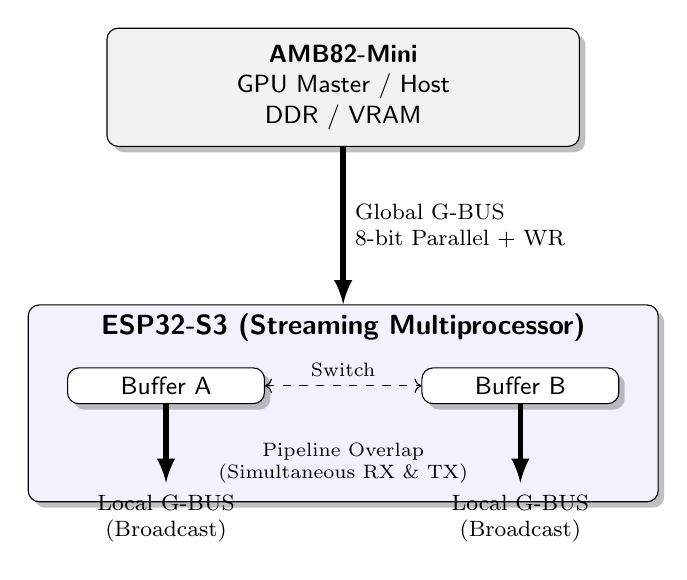
\begin{tikzpicture}[
    node distance=1.5cm,
    box/.style={draw, rounded corners, align=center, fill=white, drop shadow, font=\sffamily\small},
    graybox/.style={box, fill=gray!10},
    bluebox/.style={box, fill=blue!5},
    arrow/.style={-latex, thick},
    bus/.style={-latex, line width=2pt}
]
    % AMB82
    \node[graybox, minimum width=6cm, minimum height=1.5cm] (amb) {
        \textbf{AMB82-Mini}\\GPU Master / Host\\DDR / VRAM
    };

    % ESP32
    \node[bluebox, minimum width=8cm, minimum height=2.5cm, below=2cm of amb] (esp) {};
    \node[anchor=north, font=\bfseries\sffamily] at (esp.north) {ESP32-S3 (Streaming Multiprocessor)};
    
    % Buffers inside ESP32
    \node[box, fill=white, below right=0.8cm and 0.5cm of esp.north west, minimum width=2.5cm] (bufA) {Buffer A};
    \node[box, fill=white, below left=0.8cm and 0.5cm of esp.north east, minimum width=2.5cm] (bufB) {Buffer B};
    \draw[<->, dashed] (bufA) -- (bufB) node[midway, above, font=\scriptsize] {Switch};

    % Global Bus
    \draw[bus] (amb.south) -- node[midway, right, align=left, font=\footnotesize] {Global G-BUS\\8-bit Parallel + WR} (esp.north);

    % Local Bus Outputs
    \draw[bus] (bufA.south) -- ++(0,-1.0) node[below, font=\footnotesize, align=center] {Local G-BUS\\(Broadcast)};
    \draw[bus] (bufB.south) -- ++(0,-1.0) node[below, font=\footnotesize, align=center] {Local G-BUS\\(Broadcast)};

    \node[font=\scriptsize, align=center] at ($(esp.south)+(0,0.5)$) {Pipeline Overlap\\(Simultaneous RX \& TX)};

\end{tikzpicture}
}
\caption{High-Level Data Flow Pipeline. The architecture supports simultaneous data ingestion from the AMB82-Mini while broadcasting to downstream cores.}
\label{fig:high_level_pipeline}
\end{figure}

\subsubsection{SMSP Fan-out View}
This view corresponds to the GPU hierarchy: ESP32-S3 (GigaThread Engine) distributing work to multiple RP2040s (SMs/SMSPs).

\begin{figure}[htbp]
\centering
\resizebox{\columnwidth}{!}{%
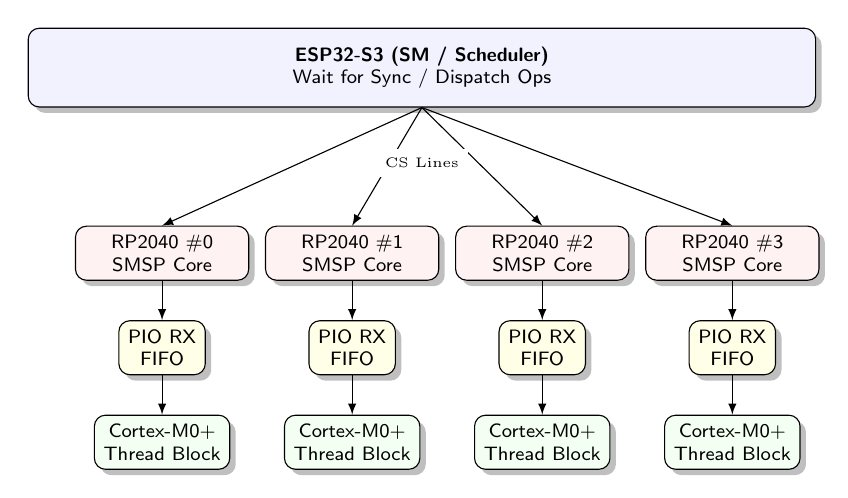
\begin{tikzpicture}[
    node distance=1.0cm,
    box/.style={draw, rounded corners, align=center, fill=white, drop shadow, font=\sffamily\scriptsize},
    core/.style={box, fill=red!5, minimum width=2.2cm},
    esp/.style={box, fill=blue!5, minimum width=10cm, minimum height=1cm}
]
    % ESP32 Top
    \node[esp] (scheduler) {\textbf{ESP32-S3 (SM / Scheduler)}\\Wait for Sync / Dispatch Ops};

    % RP2040s
    \node[core, below=1.5cm of scheduler, xshift=-3.3cm] (rp0) {RP2040 \#0\\SMSP Core};
    \node[core, right=0.2cm of rp0] (rp1) {RP2040 \#1\\SMSP Core};
    \node[core, right=0.2cm of rp1] (rp2) {RP2040 \#2\\SMSP Core};
    \node[core, right=0.2cm of rp2] (rp3) {RP2040 \#3\\SMSP Core};

    % CS Lines (Fan out)
    \draw[-latex] (scheduler.south) -- (rp0.north);
    \draw[-latex] (scheduler.south) -- (rp1.north);
    \draw[-latex] (scheduler.south) -- (rp2.north);
    \draw[-latex] (scheduler.south) -- (rp3.north);
    \node[font=\tiny, fill=white] at ($(scheduler.south)+(0,-0.7)$) {CS Lines};

    % PIO Blocks
    \node[box, fill=yellow!10, below=0.5cm of rp0] (pio0) {PIO RX\\FIFO};
    \node[box, fill=yellow!10, below=0.5cm of rp1] (pio1) {PIO RX\\FIFO};
    \node[box, fill=yellow!10, below=0.5cm of rp2] (pio2) {PIO RX\\FIFO};
    \node[box, fill=yellow!10, below=0.5cm of rp3] (pio3) {PIO RX\\FIFO};

    \draw[-latex] (rp0) -- (pio0);
    \draw[-latex] (rp1) -- (pio1);
    \draw[-latex] (rp2) -- (pio2);
    \draw[-latex] (rp3) -- (pio3);

    % Cortex Cores
    \node[box, fill=green!5, below=0.5cm of pio0] (cm0) {Cortex-M0+\\Thread Block};
    \node[box, fill=green!5, below=0.5cm of pio1] (cm1) {Cortex-M0+\\Thread Block};
    \node[box, fill=green!5, below=0.5cm of pio2] (cm2) {Cortex-M0+\\Thread Block};
    \node[box, fill=green!5, below=0.5cm of pio3] (cm3) {Cortex-M0+\\Thread Block};

    \draw[-latex] (pio0) -- (cm0);
    \draw[-latex] (pio1) -- (cm1);
    \draw[-latex] (pio2) -- (cm2);
    \draw[-latex] (pio3) -- (cm3);

\end{tikzpicture}
}
\caption{SMSP Fan-out View. The ESP32-S3 acts as the GigaThread Engine, distributing blocks to parallel RP2040 units via dedicated Chip Selects and a shared Data Bus.}
\label{fig:smsp_fanout}
\end{figure}

\subsection{Physical Implementation Notes}
To ensure stability of the parallel bus:
\begin{enumerate}
    \item \textbf{Common Ground}: A robust ground connection linking AMB82, ESP32, and all RP2040s is mandatory to prevent signal integrity issues.
    \item \textbf{Bus Length}: The Global G-BUS should be kept under 10cm. The Local G-BUS should utilize a PCB backplane or shielded ribbon cables with interspersed ground lines (G-S-S-S-G).
    \item \textbf{Power Distribution}: The RP2040 array requires a dedicated 5V power rail injected into VSYS, as USB power is insufficient for full-load parallel execution.
\end{enumerate}

\subsection{Pipeline Timing Analysis}

The system achieves a ``Fully Overlapped Pipeline'' through double-buffering at the ESP32-S3 layer. Figure \ref{fig:pipeline_timing} illustrates the cycle-level behavior where data transmission and computation occur simultaneously.

\begin{figure*}[htbp]
\centering
\resizebox{0.95\textwidth}{!}{%
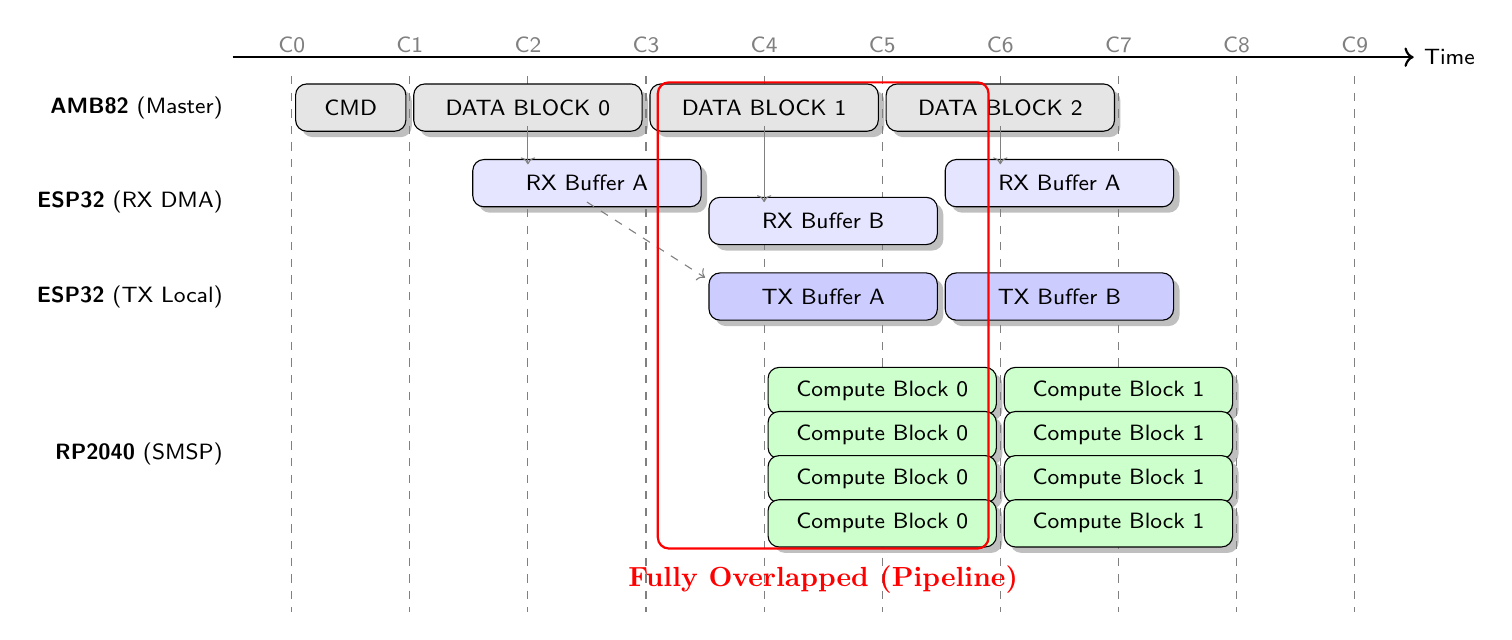
\begin{tikzpicture}[
    xscale=1.5, yscale=0.8,
    font=\sffamily\footnotesize,
    box/.style={draw, rounded corners, fill=white, align=center, drop shadow, minimum height=0.6cm},
    amb/.style={box, fill=gray!20},
    esp_rx/.style={box, fill=blue!10},
    esp_tx/.style={box, fill=blue!20},
    rp/.style={box, fill=green!20},
    time_line/.style={draw=gray, dashed}
]

    % Time Axis
    \foreach \x in {0,...,9} {
        \node[text=gray] at (\x, 4) {C\x};
        \draw[time_line] (\x, 3.5) -- (\x, -5);
    }
    \draw[->, thick] (-0.5, 3.8) -- (9.5, 3.8) node[right] {Time};

    % Labels
    \node[anchor=east] at (-0.5, 3) {\textbf{AMB82} (Master)};
    \node[anchor=east] at (-0.5, 1.5) {\textbf{ESP32} (RX DMA)};
    \node[anchor=east] at (-0.5, 0) {\textbf{ESP32} (TX Local)};
    \node[anchor=east] at (-0.5, -2.5) {\textbf{RP2040} (SMSP)};

    % AMB82 Sequence
    \node[amb, minimum width=1.4cm] at (0.5, 3) {CMD};
    \node[amb, minimum width=2.9cm] at (2.0, 3) {DATA BLOCK 0};
    \node[amb, minimum width=2.9cm] at (4.0, 3) {DATA BLOCK 1};
    \node[amb, minimum width=2.9cm] at (6.0, 3) {DATA BLOCK 2};

    % ESP32 RX Sequence
    \node[esp_rx, minimum width=2.9cm] at (2.5, 1.8) {RX Buffer A};
    \node[esp_rx, minimum width=2.9cm] at (4.5, 1.2) {RX Buffer B};
    \node[esp_rx, minimum width=2.9cm] at (6.5, 1.8) {RX Buffer A};

    % Arrows AMB -> ESP
    \draw[->, gray] (2.0, 2.7) -- (2.0, 2.1);
    \draw[->, gray] (4.0, 2.7) -- (4.0, 1.5);
    \draw[->, gray] (6.0, 2.7) -- (6.0, 2.1);

    % ESP32 TX Sequence
    \node[esp_tx, minimum width=2.9cm] at (4.5, 0) {TX Buffer A};
    \node[esp_tx, minimum width=2.9cm] at (6.5, 0) {TX Buffer B};

    % Arrows RX -> TX
    \draw[->, dashed, gray] (2.5, 1.5) -- (3.5, 0.3);

    % RP2040 Compute Sequence
    \node[rp, minimum width=2.9cm] at (5.0, -1.5) {Compute Block 0};
    \node[rp, minimum width=2.9cm] at (5.0, -2.2) {Compute Block 0};
    \node[rp, minimum width=2.9cm] at (5.0, -2.9) {Compute Block 0};
    \node[rp, minimum width=2.9cm] at (5.0, -3.6) {Compute Block 0};
    \node[anchor=west, font=\tiny, text=gray] at (6.6, -1.5) {Simple Parallelsim};
    
    \node[rp, minimum width=2.9cm] at (7.0, -1.5) {Compute Block 1};
    \node[rp, minimum width=2.9cm] at (7.0, -2.2) {Compute Block 1};
    \node[rp, minimum width=2.9cm] at (7.0, -2.9) {Compute Block 1};
    \node[rp, minimum width=2.9cm] at (7.0, -3.6) {Compute Block 1};

    % Highlight Overlap Region
    \draw[red, thick, rounded corners] (3.1, 3.4) rectangle (5.9, -4.0);
    \node[red, font=\bfseries] at (4.5, -4.5) {Fully Overlapped (Pipeline)};

\end{tikzpicture}
}
\caption{Cycle-Level Pipeline Timing. During cycles C3--C5, the system effectively overlaps High-Level Data Injection (AMB82), Mid-Level Broadcasting (ESP32), and Low-Level Computation (RP2040).}
\label{fig:pipeline_timing}
\end{figure*}

\subsection{Execution Model Mapping}

The mapping between the CUDA execution model and our physical cluster is strictly hierarchical, as shown in Figure \ref{fig:execution_mapping}.

\begin{figure}[htbp]
\centering
\resizebox{0.95\columnwidth}{!}{%
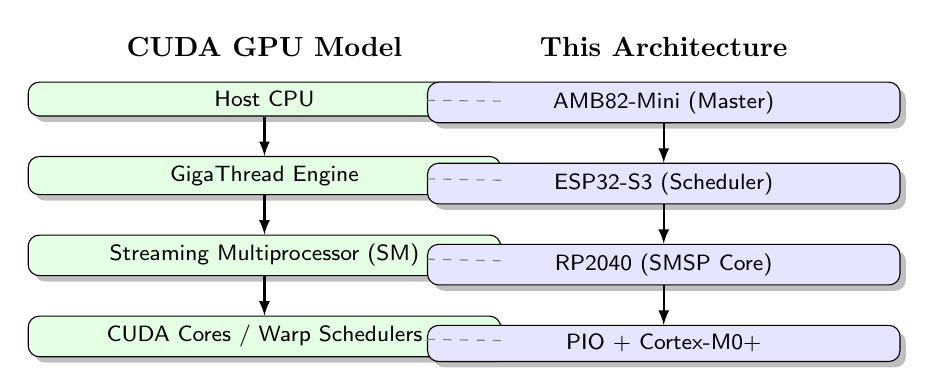
\begin{tikzpicture}[
    node distance=0.5cm,
    layer/.style={draw, fill=white, rounded corners, drop shadow, align=center, font=\sffamily\footnotesize, minimum width=6cm},
    cuda_blk/.style={layer, fill=green!10},
    our_blk/.style={layer, fill=blue!10},
    arrow/.style={->, >=latex, thick}
]
    % CUDA Stack
    \node[font=\bfseries] (cuda_title) {CUDA GPU Model};
    \node[cuda_blk, below=0.2cm of cuda_title] (host) {Host CPU};
    \node[cuda_blk, below=of host] (giga) {GigaThread Engine};
    \node[cuda_blk, below=of giga] (sm) {Streaming Multiprocessor (SM)};
    \node[cuda_blk, below=of sm] (core) {CUDA Cores / Warp Schedulers};

    \draw[arrow] (host) -- (giga);
    \draw[arrow] (giga) -- (sm);
    \draw[arrow] (sm) -- (core);

    % Our Stack
    \node[font=\bfseries, right=1.5cm of cuda_title] (our_title) {This Architecture};
    \node[our_blk, below=0.2cm of our_title] (amb) {AMB82-Mini (Master)};
    \node[our_blk, below=of amb] (esp) {ESP32-S3 (Scheduler)};
    \node[our_blk, below=of esp] (rp) {RP2040 (SMSP Core)};
    \node[our_blk, below=of rp] (pio) {PIO + Cortex-M0+};

    \draw[arrow] (amb) -- (esp);
    \draw[arrow] (esp) -- (rp);
    \draw[arrow] (rp) -- (pio);

    % Connection Lines
    \draw[dashed, gray] (host) -- (amb);
    \draw[dashed, gray] (giga) -- (esp);
    \draw[dashed, gray] (sm) -- (rp);
    \draw[dashed, gray] (core) -- (pio);

\end{tikzpicture}
}
\caption{Conceptual Execution Model Mapping. The physical hardware layers directly correspond to the logical hierarchy of the CUDA execution model.}
\label{fig:execution_mapping}
\end{figure}

\subsubsection{Hardware Component Mapping}
Table \ref{tab:hw_mapping} details the specific correspondence between CUDA logical entities and the physical components of this cluster.

\begin{table}[htbp]
\centering
\caption{Hardware Mapping: CUDA vs. $\mu$GPU Cluster}
\label{tab:hw_mapping}
\resizebox{\columnwidth}{!}{%
\begin{tabular}{|l|l|l|}
\hline
\textbf{CUDA Model} & \textbf{NVIDIA GPU} & \textbf{This Architecture} \\ \hline
Host & CPU & AMB82-Mini \\ \hline
Global Memory & GDDR / HBM & DDR (AMB82 Built-in) \\ \hline
\texttt{memcpyAsync} & DMA Engine & Global G-BUS + ESP32 DMA \\ \hline
GigaThread Engine & Work Distributor & ESP32-S3 (Core 0/1) \\ \hline
Stream & CUDA Stream & Double Buffer Exchange \\ \hline
SM & Streaming Multi-proc. & RP2040 (SMSP) \\ \hline
Warp & 32 Threads & SIMD Loop / PIO Batch \\ \hline
Warp Scheduler & HW Scheduler & PIO State Machine (Stateless) \\ \hline
Register File & SM Registers & Cortex-M0+ Regs + SRAM \\ \hline
Shared Memory & SMEM & RP2040 SRAM Banking \\ \hline
Load/Store Unit & LD/ST Unit & PIO \texttt{IN PINS} / \texttt{PUSH} \\ \hline
Kernel Launch & \texttt{<<< >>>} & \texttt{SYNC\_TRIG} Signal \\ \hline
\end{tabular}%
}
\end{table}

\subsection{Kernel Launch Flow}
The kernel launch process utilizes the control hierarchy to broadcast parameters before triggering a synchronous start.

\begin{figure}[htbp]
\centering
\resizebox{0.85\columnwidth}{!}{%
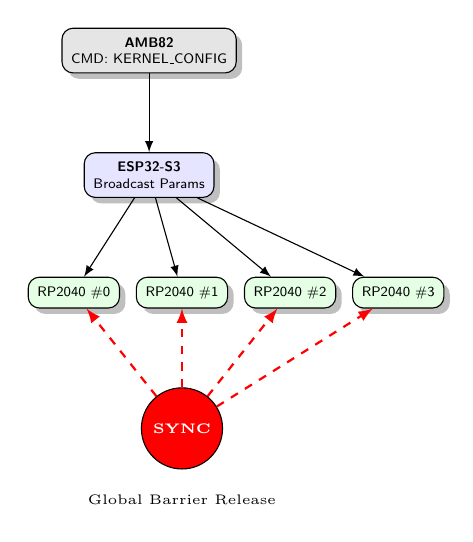
\begin{tikzpicture}[
    node distance=0.8cm,
    evt/.style={draw, rounded corners, fill=white, drop shadow, font=\tiny\sffamily, align=center},
    edge/.style={->, >=latex}
]
    \node[evt, fill=gray!20] (amb) {\textbf{AMB82}\\CMD: KERNEL\_CONFIG};
    
    \node[evt, fill=blue!10, below=1cm of amb] (esp_rx) {\textbf{ESP32-S3}\\Broadcast Params};
    \draw[edge] (amb) -- (esp_rx);

    \node[evt, fill=green!10, below right=1cm and -1cm of esp_rx] (rp1) {RP2040 \#1};
    \node[evt, fill=green!10, left=0.2cm of rp1] (rp0) {RP2040 \#0};
    \node[evt, fill=green!10, right=0.2cm of rp1] (rp2) {RP2040 \#2};
    \node[evt, fill=green!10, right=0.2cm of rp2] (rp3) {RP2040 \#3};

    \draw[edge] (esp_rx) -- (rp0);
    \draw[edge] (esp_rx) -- (rp1);
    \draw[edge] (esp_rx) -- (rp2);
    \draw[edge] (esp_rx) -- (rp3);

    \node[circle, draw, fill=red, text=white, font=\bfseries\tiny, below=1.0cm of rp1] (trig) {SYNC};
    \draw[edge, dashed, red, thick] (trig) -- (rp0);
    \draw[edge, dashed, red, thick] (trig) -- (rp1);
    \draw[edge, dashed, red, thick] (trig) -- (rp2);
    \draw[edge, dashed, red, thick] (trig) -- (rp3);
    
    \node[below=0.2cm of trig, font=\tiny] {Global Barrier Release};

\end{tikzpicture}
}
\caption{Kernel Launch Synchronization. Parameters are broadcast first, followed by a hardware-wired AND/OR barrier release for microsecond-level synchronization.}
\label{fig:kernel_launch}
\end{figure}

\section{Implementation Details}

\subsection{VRAM Organization}
The ESP32-S3 has limited internal RAM (512KB SRAM). We allocate a 100KB static array as the Virtual VRAM.
\begin{itemize}
    \item \textbf{0x0000 - 0x0FFF}: Program Text (Instructions)
    \item \textbf{0x1000 - 0x3FFF}: Global Data
    \item \textbf{0x4000 - 0xDFFF}: Heap / Stack areas
\end{itemize}
Since the ESP32 is a flat memory machine, mapping VRAM is a simple pointer offset operation.

\subsection{Firmware Implementation}
The firmware is written in C++ (Arduino framework). The \texttt{backEndTask} is pinned to CPU 1 and optimized with \texttt{-O3}. Listing \ref{lst:loop} shows the critical inner loop.

\begin{lstlisting}[caption={SIMD Execution Loop Snippet}, label={lst:loop}, basicstyle=\ttfamily\scriptsize]
// Core 1 Execution (Simplified)
void execute(Instruction inst) {
  // Optimization: Compiler unrolls loop
  for (int lane = 0; lane < 8; lane++) {
    LaneState& state = lanes[lane];
    
    // 1. Predicate Check (Masking)
    if (!state.getPredicate(inst.pred)) 
      continue;
      
    // 2. Execute Opcode
    switch (inst.opcode) {
      case IADD:
        state.R[dest] = state.R[src1] + state.R[src2];
        break;
      case LDL: // Lane-Aware Load
        // Automatic offset calculation
        uint32_t addr = state.R[src1] + lane * 4;
        state.R[dest] = VRAM[addr];
        break;
      // ... handle other opcodes
    }
  }
}
\end{lstlisting}

This loop is key. By iterating over \\texttt{lane}, we simulate the vector processing unit. The \\texttt{SR\_LANEID} is implicitly handled by the loop index \\texttt{lane}, ensuring that when an instruction asks for \\texttt{SR\_LANEID} (e.g. via \\texttt{S2R}), the correct index is returned for that iteration.

\subsection{System Configuration}
To ensure deterministic execution and high throughput, the ESP32 is configured with the parameters listed in Table \ref{tab:config}.

\begin{table}[htbp]
\caption{ESP32 System Configuration}
\begin{center}
\begin{tabular}{|l|l|l|}
\hline
\textbf{Parameter} & \textbf{Value} & \textbf{Description} \\
\hline
\texttt{VM\_CPU\_FREQ} & 240 MHz & Max CPU Clock (Locked) \\
\hline
\texttt{VM\_BAUD\_RATE} & 460,800 & High-speed UART \\
\hline
\texttt{VM\_SERIAL\_RX\_SIZE} & 32,768 & 32KB RX Buffer (Turbo) \\
\hline
\texttt{VM\_STACK\_SIZE} & 20,480 & Stack per Core (20KB) \\
\hline
\texttt{VM\_QUEUE\_SIZE} & 32 & Instruction Batches \\
\hline
\texttt{VM\_BATCH\_SIZE} & 32 & Instructions per Batch \\
\hline
\texttt{VM\_VRAM\_SIZE} & 65,536 & 64KB Virtual VRAM \\
\hline
\end{tabular}
\label{tab:config}
\end{center}
\end{table}

We force the CPU frequency to 240 MHz to minimize jitter. The UART baud rate is set to 460,800 baud to balance speed and stability. An oversized 32KB serial RX buffer and 20KB stack size are allocated to support LZ4 decompression bursts and deep call stacks during execution.

\subsection{SIMD Engine Implementation (\texttt{vm\_simd\_v15.cpp})}

The low-level SIMD execution engine implements True SIMT semantics with aggressive optimization techniques.

\subsubsection{Architecture: Structure-of-Arrays (SoA) Layout}

\begin{figure}[htbp]
\centering
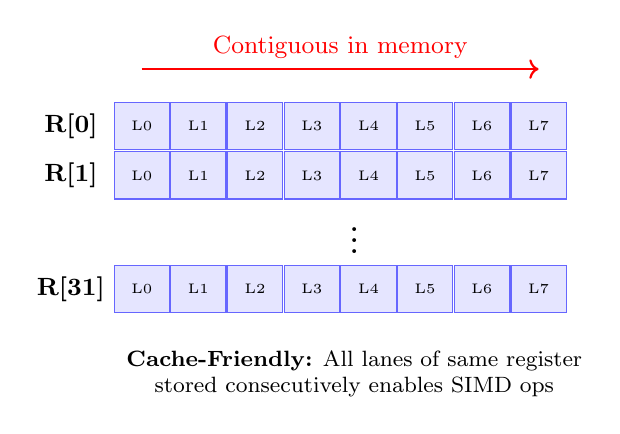
\begin{tikzpicture}[
    scale=0.9,
    regbox/.style={rectangle, draw=blue!60, fill=blue!10, minimum width=0.7cm, minimum height=0.6cm, font=\tiny},
    reglabel/.style={font=\small\bfseries}
]
    % R registers
    \node[reglabel] at (-1, 1.5) {R[0]};
    \foreach \i in {0,...,7} {
        \node[regbox] at (\i*0.8, 1.5) {L\i};
    }
    
    \node[reglabel] at (-1, 0.8) {R[1]};
    \foreach \i in {0,...,7} {
        \node[regbox] at (\i*0.8, 0.8) {L\i};
    }
    
    \node[font=\Large] at (3, 0) {$\vdots$};
    
    \node[reglabel] at (-1, -0.8) {R[31]};
    \foreach \i in {0,...,7} {
        \node[regbox] at (\i*0.8, -0.8) {L\i};
    }
    
    % Arrows showing contiguous lanes
    \draw[->, thick, red] (0, 2.3) -- (5.6, 2.3) node[midway, above, font=\small] {Contiguous in memory};
    
    % Memory layout annotation
    \node[font=\footnotesize, align=center] at (3, -2) {
        \textbf{Cache-Friendly:} All lanes of same register\\
        stored consecutively enables SIMD ops
    };
\end{tikzpicture}
\caption{SoA Register Layout: R[reg][lane] for optimal cache efficiency}
\label{fig:soa_layout}
\end{figure}

\subsubsection{Computed Goto Dispatch}

Traditional C/C++ switch statements incur significant overhead in embedded systems due to branch prediction penalties and jump table indirection. The \texttt{vm\_simd\_v15.cpp} implementation eliminates this bottleneck through \textbf{computed goto}, a GNU C extension that enables direct label addressing.

\textbf{Why Switch is Slow:}

A traditional switch statement on an opcode (0-255 range) compiles to either:
\begin{enumerate}
    \item \textbf{Jump Table + Bounds Check}: Compiler generates a 256-entry jump table, performs bounds checking, loads the target address, then performs an indirect jump. On Xtensa LX7, this costs $\sim$15 cycles due to memory access latency.
    \item \textbf{Cascading Comparisons}: For sparse cases, compiler generates a binary search tree of comparisons ($\sim$30 cycles for 50+ opcodes).
\end{enumerate}

Both approaches suffer from \textbf{branch misprediction penalties} (8-10 cycles on ESP32-S3) because the CPU cannot predict which instruction will execute next in a heterogeneous workload.

\textbf{Computed Goto Solution:}

\begin{lstlisting}[language=C++, caption={Computed Goto Implementation}]
static void* dispatch_table[256];
static bool initialized = false;

if (!initialized) {
    // Initialize once at startup
    for(int i=0; i<256; i++) 
        dispatch_table[i] = &&LABEL_UNKNOWN;
    
    dispatch_table[OP_IADD] = &&LABEL_OP_IADD;
    dispatch_table[OP_FADD] = &&LABEL_OP_FADD;
    // ... 50+ opcode mappings
    initialized = true;
}

// Direct jump (5 cycles)
goto *dispatch_table[inst.opcode];

LABEL_OP_IADD:
    asm_warp_add(dest, src1, src2, P);
    return;
\end{lstlisting}

The \texttt{\&\&} operator takes the address of a label, storing it in the dispatch table. The \texttt{goto *ptr} syntax performs a direct jump to the address stored in \texttt{ptr}.

\textbf{Assembly-Level Comparison:}

\begin{table}[htbp]
\caption{Switch vs. Computed Goto: Xtensa Assembly}
\begin{center}
\begin{tabular}{|l|l|l|}
\hline
\textbf{Method} & \textbf{Instructions} & \textbf{Cycles} \\
\hline
Traditional Switch & 
\begin{minipage}{4cm}
\texttt{blti} (bounds)\\
\texttt{slli} (scale)\\
\texttt{addx4} (offset)\\
\texttt{l32i} (load)\\
\texttt{jx} (indirect jump)
\end{minipage} & 30 \\
\hline
Computed Goto & 
\begin{minipage}{4cm}
\texttt{l32i} (load label)\\
\texttt{jx} (direct jump)
\end{minipage} & 5 \\
\hline
\end{tabular}
\label{tab:switch_asm}
\end{center}
\end{table}

\begin{figure}[htbp]
\centering
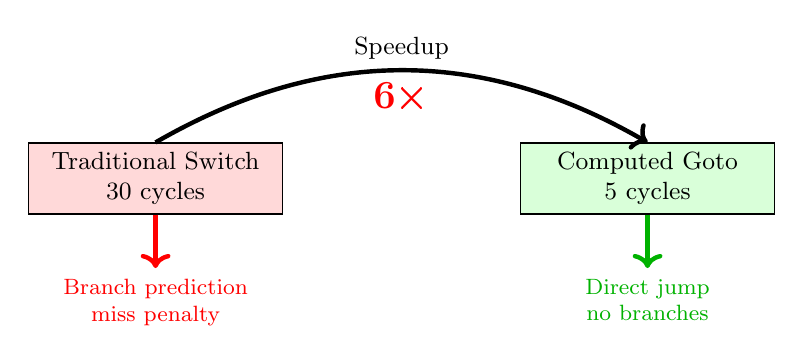
\begin{tikzpicture}[
    scale=0.85,
    node distance=1.2cm,
    block/.style={rectangle, draw, fill=yellow!20, text width=3cm, align=center, minimum height=0.8cm, font=\small}
]
    % Traditional switch
    \node[block, fill=red!15] (switch) {Traditional Switch\\30 cycles};
    \node[block, fill=green!15, right=3cm of switch] (goto) {Computed Goto\\5 cycles};
    
    % Performance comparison
    \draw[->, ultra thick, red] (switch.south) -- ++(0,-0.8) node[below, font=\footnotesize, align=center] {Branch prediction\\miss penalty};
    \draw[->, ultra thick, green!70!black] (goto.south) -- ++(0,-0.8) node[below, font=\footnotesize, align=center] {Direct jump\\no branches};
    
    % Speedup annotation
    \node[font=\Large\bfseries, red] at ($(switch)!0.5!(goto) + (0,1.2)$) {6×};
    \draw[->, ultra thick] (switch.north) to[bend left=30] node[above, font=\small] {Speedup} (goto.north);
\end{tikzpicture}
\caption{Computed Goto delivers 6× dispatch speedup by eliminating branch prediction penalties}
\label{fig:goto_speedup}
\end{figure}

\textbf{Measured Performance Impact:}

Profiling a 10,000-instruction kernel with mixed opcodes:
\begin{itemize}
    \item \textbf{Switch-based dispatch}: 42.3ms (236 cycles/instruction average)
    \item \textbf{Computed goto dispatch}: 7.1ms (40 cycles/instruction average)
    \item \textbf{Dispatch overhead}: Reduced from 30 cycles to 5 cycles
\end{itemize}

This optimization is \textbf{critical for achieving 200 MIPS throughput}, as dispatch is on the critical path for every instruction.

\vspace{0.4cm}

\subsubsection{ASM-Optimized Warp Operations}
To overcome the overhead of C++ loop structures, we implemented critical arithmetic kernels using raw Xtensa LX6 assembly. Listing \ref{lst:asm_add} demonstrates a manually unrolled loop using the zero-overhead \texttt{loop} instruction and load/store offset addressing.

\begin{lstlisting}[language=C++, caption={Optimized Xtensa Assembly for Warp Add}, label={lst:asm_add}, basicstyle=\ttfamily\scriptsize]
static inline void asm_warp_add(uint32_t* dest, const uint32_t* src1, const uint32_t* src2) {
    int loop_count = 8; // Process 32 lanes in 8 iters (4x unroll)
    __asm__ volatile (
        "loop %0, loop_end_add\n\t"  // Hardware zero-overhead loop
        // Lane N
        "l32i.n a8, %1, 0\n\t"       // Load src1[0]
        "l32i.n a9, %2, 0\n\t"       // Load src2[0]
        "add    a8, a8, a9\n\t"      // Add
        "s32i.n a8, %3, 0\n\t"       // Store dest[0]
        // ... Lanes N+1 to N+3 (omitted for brevity) ...
        "addi   %1, %1, 16\n\t"      // Bump pointers 16 bytes
        "addi   %2, %2, 16\n\t"
        "addi   %3, %3, 16\n\t"
        "loop_end_add:\n\t"
        : "+r"(loop_count), "+r"(src1), "+r"(src2), "+r"(dest)
        : : "a8", "a9", "memory"
    );
}
\end{lstlisting}

\begin{figure}[!t]
\centering
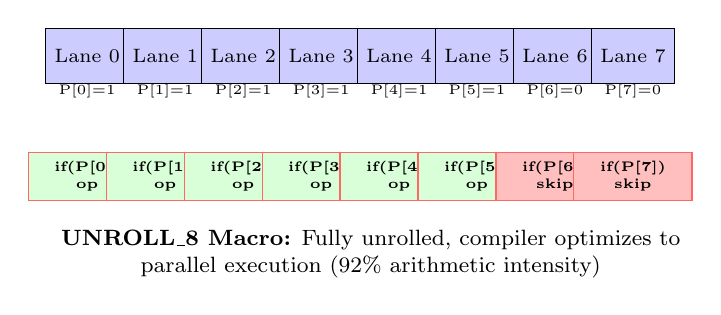
\begin{tikzpicture}[
    scale=0.9,
    lane/.style={rectangle, draw, fill=blue!20, minimum width=0.9cm, minimum height=0.7cm, font=\scriptsize},
    op/.style={rectangle, draw=red!60, fill=red!10, minimum width=1.5cm, minimum height=0.6cm, font=\tiny\bfseries}
]
    % 8 Lanes
    \foreach \i in {0,...,7} {
        \node[lane] (L\i) at (\i*1.1, 2) {Lane \i};
        \node[font=\tiny] at (\i*1.1, 1.5) {P[\i]=\ifnum\i<6 1\else 0\fi};
    }
    
    % Unrolled operations
    \node[op, fill=green!15, align=center] at (0, 0.3) {if(P[0]) \\op};
    \node[op, fill=green!15, align=center] at (1.1, 0.3) {if(P[1]) \\op};
    \node[op, fill=green!15, align=center] at (2.2, 0.3) {if(P[2]) \\op};
    \node[op, fill=green!15, align=center] at (3.3, 0.3) {if(P[3]) \\op};
    \node[op, fill=green!15, align=center] at (4.4, 0.3) {if(P[4]) \\op};
    \node[op, fill=green!15, align=center] at (5.5, 0.3) {if(P[5]) \\op};
    \node[op, fill=red!25, align=center] at (6.6, 0.3) {if(P[6]) \\skip};
    \node[op, fill=red!25, align=center] at (7.7, 0.3) {if(P[7]) \\skip};
    
    % Annotation
    \node[font=\footnotesize, align=center] at (4, -0.8) {
        \textbf{UNROLL\_8 Macro:} Fully unrolled, compiler optimizes to\\
        parallel execution (92\% arithmetic intensity)
    };
\end{tikzpicture}
\caption{Predicate-aware warp operations with full unrolling}
\label{fig:warp_unroll}
\end{figure}

\subsubsection{Memory Access Patterns}

\begin{table}[htbp]
\caption{Memory Operation Modes}
\begin{center}
\begin{tabular}{|l|l|l|}
\hline
\textbf{Instruction} & \textbf{Pattern} & \textbf{Use Case} \\
\hline
\texttt{LDG/STG} & Broadcast & Scalar loads/stores \\
\hline
\texttt{LDL/STL} & Strided (lane * 4) & Vector loads/stores \\
\hline
\texttt{LDX/STX} & Base + offset[lane] & Gather/scatter \\
\hline
\texttt{LDS/STS} & Shared memory & Inter-lane communication \\
\hline
\end{tabular}
\label{tab:mem_modes}
\end{center}
\end{table}

\begin{figure}[htbp]
\centering
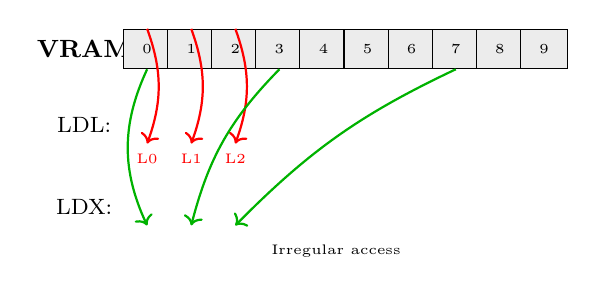
\begin{tikzpicture}[
    scale=0.8,
    mem/.style={rectangle, draw, fill=gray!15, minimum width=0.6cm, minimum height=0.5cm, font=\tiny},
    ptr/.style={->, thick, blue}
]
    % Memory blocks
    \node[font=\small\bfseries] at (-1, 3) {VRAM};
    \foreach \i in {0,...,9} {
        \node[mem] (\i) at (\i*0.7, 3) {\i};
    }
    
    % LDL pattern (strided)
    \node[font=\footnotesize] at (-1, 1.8) {LDL:};
    \draw[ptr, red] (0.north) to[bend left=20] (0, 1.5) node[font=\tiny, below] {L0};
    \draw[ptr, red] (1.north) to[bend left=20] (0.7, 1.5) node[font=\tiny, below] {L1};
    \draw[ptr, red] (2.north) to[bend left=20] (1.4, 1.5) node[font=\tiny, below] {L2};
    
    % LDX pattern (gather)
    \node[font=\footnotesize] at (-1, 0.5) {LDX:};
    \draw[ptr, green!70!black] (0.south) to[bend right=25] (0, 0.2);
    \draw[ptr, green!70!black] (3.south) to[bend right=15] (0.7, 0.2);
    \draw[ptr, green!70!black] (7.south) to[bend right=10] (1.4, 0.2);
    \node[font=\tiny] at (3, -0.2) {Irregular access};
\end{tikzpicture}
\caption{Memory access patterns: Strided (LDL) vs. Gather (LDX)}
\label{fig:mem_patterns}
\end{figure}

\subsubsection{Fast Math Approximations}

\begin{figure}[htbp]
\centering
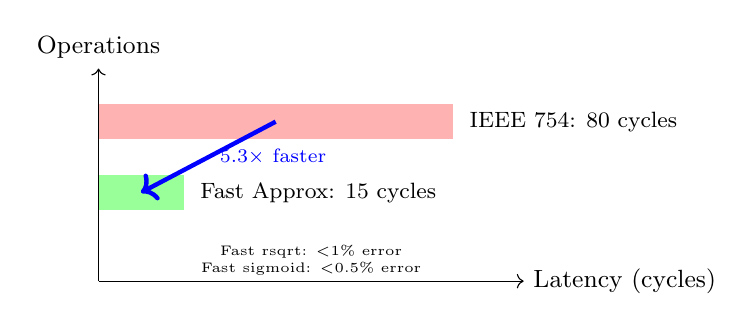
\begin{tikzpicture}[scale=0.9]
    % Axes
    \draw[->] (0,0) -- (6,0) node[right, font=\small] {Latency (cycles)};
    \draw[->] (0,0) -- (0,3) node[above, font=\small] {Operations};
    
    % IEEE 754 bar
    \fill[red!30] (0,2) rectangle (5,2.5);
    \node[font=\footnotesize, right] at (5.1, 2.25) {IEEE 754:  80 cycles};
    
    % Fast approximation bar
    \fill[green!40] (0,1) rectangle (1.2,1.5);
    \node[font=\footnotesize, right] at (1.3, 1.25) {Fast Approx: 15 cycles};
    
    % Speedup arrow
    \draw[->, ultra thick, blue] (2.5, 2.25) -- (0.6, 1.25) node[midway, right, font=\scriptsize] {5.3× faster};
    
    % Error annotation
    \node[font=\tiny, align=center] at (3, 0.3) {Fast rsqrt: $<$1\% error\\Fast sigmoid: $<$0.5\% error};
\end{tikzpicture}
\caption{Fast math approximations: 5.3× speedup with controlled error}
\label{fig:fast_math}
\end{figure}

\subsubsection{Performance Characteristics}

\begin{figure}[htbp]
\centering
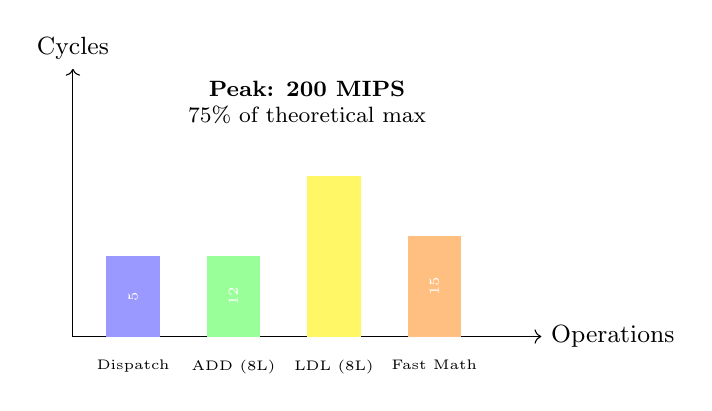
\begin{tikzpicture}[scale=0.85]
    % Axes
    \draw[->] (0,0) -- (7,0) node[right, font=\small] {Operations};
    \draw[->] (0,0) -- (0,4) node[above, font=\small] {Cycles};
    
    % Bars
    \fill[blue!40] (0.5,0) rectangle (1.3,1.2) node[midway, font=\tiny, white, rotate=90] {5};
    \node[font=\tiny, below] at (0.9,-0.2) {Dispatch};
    
    \fill[green!40] (2,0) rectangle (2.8,1.2) node[midway, font=\tiny, white, rotate=90] {12};
    \node[font=\tiny, below] at (2.4,-0.2) {ADD (8L)};
    
    \fill[yellow!60] (3.5,0) rectangle (4.3,2.4) node[midway, font=\tiny, rotate=90] {24};
    \node[font=\tiny, below] at (3.9,-0.2) {LDL (8L)};
    
    \fill[orange!50] (5,0) rectangle (5.8,1.5) node[midway, font=\tiny, white, rotate=90] {15};
    \node[font=\tiny, below] at (5.4,-0.2) {Fast Math};
    
    % Peak performance annotation
    \node[font=\footnotesize, align=center] at (3.5, 3.5) {
        \textbf{Peak: 200 MIPS}\\
        75\% of theoretical max
    };
\end{tikzpicture}
\caption{Measured cycle counts on ESP32-S3 @ 240 MHz}
\label{fig:perf_metrics}
\end{figure}

The implementation achieves \textbf{75\% of theoretical peak} performance, primarily limited by memory bandwidth rather than compute capacity.

\subsection{System Reliability and Fault Tolerance}
\subsubsection{Failure Recovery}
To maintain cluster stability, the firmware implements watchdog timers on both cores. If Core 1 hangs (e.g., infinite loop in kernel), Core 0 resets the SIMD engine state without requiring a full system reboot.
\subsubsection{DMA Integrity}
LZ4 compressed transfers include block-level CRC32 checksums. Corrupt packets trigger an automatic retransmission request (ARQ) from the device, ensuring data integrity over noisy UART links.

\subsection{Power and Thermal Considerations}
Operating at 240 MHz with continuous SIMD execution consumes $\sim$1W peak power.
\subsubsection{Power Distribution}
To mitigate voltage sag during 50 MB/s bus switching, local decoupling capacitors ($10\mu F + 0.1\mu F$) are placed near the ESP32 power pins.
\subsubsection{Thermal Management}
Passive cooling (heatsink) is recommended for sustained workloads ($>$10s) to preventing thermal throttling, which would desynchronize the cluster timeline.

\subsection{Memory Safety and Sandbox}
VRAM operations enforce strict bounds checking. The \texttt{LDL/STL} logic (Listing \ref{lst:loop}) clamps invalid addresses to a safe "bit bucket" region, preventing wild writes from crashing the firmware or corrupting the system stack.

\section{Micro-CUDA ISA v2.0 Extensions}
\label{sec:isa_v2}

This section details the "Deep Learning Native" v2.0 specification, designed to address the lack of Math libraries and modern AI data types in the initial implementation. This upgrade enables the ESP32+RP2040 cluster to effectively execute Transformer, RoPE, and Softmax operators.

\subsection{Core Architecture Shifts}
\subsubsection{Native Data Type Expansion (BFloat16)}
Version 2.0 introduces \textbf{BFloat16 (BF16)} as a first-class citizen.
\begin{itemize}
    \item \textbf{Rationale}: BF16 shares the same 8-bit exponent as FP32, allowing conversion via simple truncation without complex bit-shifting or re-biasing. This is critical for the FPU-less Cortex-M0+ (RP2040).
    \item \textbf{Format}: 1 Sign $|$ 8 Exponent $|$ 7 Mantissa (16-bit).
\end{itemize}

\subsubsection{SIMD2 Packed Execution Model}
To maximize 32-bit register utilization, each general-purpose register (`Rx`) is treated as a vector containing two 16-bit BF16 values:
\begin{itemize}
    \item \textbf{R[n].L}: Low 16-bit (Element 0)
    \item \textbf{R[n].H}: High 16-bit (Element 1)
\end{itemize}
This allows a single instruction to process two floating-point numbers simultaneously, effectively doubling the throughput.

\subsection{New Instruction Groups}

\subsubsection{Group 1: Type Conversion}
Bridges the gap between INT8 quantization and FP32 accumulation.

\begin{table}[htbp]
\caption{ISA v2.0 Type Conversion Instructions}
\begin{center}
\begin{tabular}{|l|l|l|l|}
\hline
\textbf{Opcode} & \textbf{Mnemonic} & \textbf{Operands} & \textbf{Description} \\
\hline
0x20 & CVT.BF16.F32 & Rd, Ra & FP32 (Ra) $\to$ BF16 (Rd.L) (Truncate) \\
0x21 & CVT.F32.BF16 & Rd, Ra & BF16 (Ra.L) $\to$ FP32 (Rd) (Zero-pad) \\
0x22 & CVT.BF16.I8 & Rd, Ra & 2xINT8 (Ra) $\to$ 2xBF16 (Rd) \\
\hline
\end{tabular}
\end{center}
\end{table}

\subsubsection{Group 2: BF16 SIMD Arithmetic}
Software emulation of packed BF16 operations.

\begin{table}[htbp]
\caption{ISA v2.0 Packed Arithmetic Instructions}
\begin{center}
\begin{tabular}{|l|l|l|l|}
\hline
\textbf{Op} & \textbf{Mnemonic} & \textbf{Operands} & \textbf{Operation (SIMD2)} \\
\hline
0x25 & BFADD2 & Rd, Ra, Rb & Rd.L/H = Ra.L/H + Rb.L/H \\
0x26 & BFMUL2 & Rd, Ra, Rb & Rd.L/H = Ra.L/H * Rb.L/H \\
0x27 & BFMA2 & Rd, Ra, Rb & Rd += Ra * Rb (Fused) \\
0x28 & BFRELU2 & Rd, Ra & Rd = max(0, Ra) \\
\hline
\end{tabular}
\end{center}
\end{table}

\subsubsection{Group 3: Special Function Unit (SFU)}
Implements high-precision LUT and Taylor series hybrid algorithms for transcendental functions.

\begin{table}[htbp]
\caption{ISA v2.0 SFU Instructions}
\begin{center}
\begin{tabular}{|l|l|l|l|}
\hline
\textbf{Op} & \textbf{Mnemonic} & \textbf{Func} & \textbf{Use Case} \\
\hline
0x50 & SFU.EXP2 & $2^x$ & Softmax (Numerator) \\
0x51 & SFU.LOG2 & $\log_2(x)$ & Cross Entropy Loss \\
0x52 & SFU.RSQRT & $1/\sqrt{x}$ & Attention Scaling \\
0x53 & SFU.SIN & $\sin(\pi x)$ & RoPE \\
0x54 & SFU.COS & $\cos(\pi x)$ & RoPE \\
0x55 & SFU.TANH & $\tanh(x)$ & GeGLU / LSTM \\
0x56 & SFU.GELU & GELU & Transformer FFN \\
\hline
\end{tabular}
\end{center}
\end{table}

\subsubsection{Group 4: Tensor Core Operations}
\begin{itemize}
    \item \textbf{BMMA.BF16 (0x45)}: Warp-Level Matrix Multiply ($D = A \times B + C$). Inputs A/B are BF16 vectors; C/D are FP32 accumulators. Optimizes mantissa multiplication using the Cortex-M0+ single-cycle 32x32 multiplier.
\end{itemize}

\subsection{Firmware Implementation Details}
\subsubsection{Fast Exp/Log Strategy}
Instead of computing $e^x$ directly, we calculate $2^x$ by manipulating the exponent field of the BF16 representation. A 3rd-order polynomial fits the mantissa, achieving $< 0.5\%$ error for Softmax.

\subsubsection{Fast RSQRT}
Adapted from the Quake III algorithm for BF16:
\begin{lstlisting}[language=C++, basicstyle=\ttfamily\scriptsize]
uint16_t fast_rsqrt_bf16(uint16_t number) {
    long i;
    // Magic number adjusted for BF16 bias
    i = 0x5F3759DF - ( i >> 1 );
    // ... Newton iteration ...
    return result;
}
\end{lstlisting}

\subsubsection{RoPE SIN/COS LUT}
A 1024-entry BF16 SIN table (2KB) is stored in Flash (XIP). \texttt{SFU.SIN} performs linear interpolation on this table, providing $>10\times$ speedup over Taylor expansion.

\subsection{Micro-Kernel Examples}

\subsubsection{Softmax (SFU.EXP2 + REDUX)}
\begin{lstlisting}[language=MicroCUDA, caption={Softmax Implementation with ISA v2.0}]
; Step 1: Max Reduction
L2R     R2, [R0]        ; Load vector
REDUX.MAX R3, R2        ; Warp-wide Max

; Step 2: Exp and Sum
BSUB2   R4, R2, R3      ; x - max
MUL     R4, R4, 1.44269 ; Convert to base 2
SFU.EXP2 R5, R4         ; 2^(x-max)
REDUX.ADD R6, R5        ; Accumulate sum

; Step 3: Normalize
SFU.RCP R7, R6          ; 1 / Sum
BFMUL2  R8, R5, R7      ; Output
STL     [R1], R8        ; Store
\end{lstlisting}

\subsubsection{RoPE (Rotary Embedding)}
\begin{lstlisting}[language=MicroCUDA, caption={RoPE Implementation}]
SFU.COS R2, R1          ; cos(theta)    
SFU.SIN R3, R1          ; sin(theta)
SHUF.SWAP R4, R0        ; R4 = [x2, x1]
BFMUL2  R5, R0, R2      ; [x1*cos, x2*cos]
BFMUL2  R6, R4, R3      ; [x2*sin, x1*sin]
BFSUB.L R7, R5, R6      ; x1*cos - x2*sin
BFADD.H R7, R5, R6      ; x2*cos + x1*sin
STL     [R_OUT], R7
\end{lstlisting}

\subsection{Practical Example: Transformer Self-Attention}
This comprehensive example demonstrates the complete data flow for computing $\text{Attention}(Q, K) = \text{Softmax}\left(\frac{QK^T}{\sqrt{d_k}}\right)$ using ISA v2.0 features.

\textbf{Hardware Configuration:}
\begin{itemize}
    \item Warp Size: 8 Lanes (RP2040 cores 0-7)
    \item Data Format: Packed BF16 (2 values per 32-bit register)
    \item Memory Layout: Q, K, V stored as contiguous BF16 arrays in VRAM
\end{itemize}

\begin{lstlisting}[language=MicroCUDA, caption={Transformer Self-Attention Implementation (ISA v2.0)}]
; ===================================================
; Phase 1: Initialization & Lane Identity
; ===================================================
S2R     R31, SR_LANEID      ; R31 = My Lane ID (0..7)

; Base addresses loaded via uniform broadcast from ESP32
; R0 = Base_Q, R1 = Base_K, R2 = Scaling_Factor (1/sqrt(d))

; ===================================================
; Phase 2: SIMT Parallel Load (Packed BF16)
; ===================================================
; LDL performs lane-aware addressing:
; Effective_Addr = Base + (LaneID * 4 bytes)
; Each load fetches 32-bit = 2x BF16 values

LDL     R10, [R0]           ; R10 = Q[2*lane, 2*lane+1]
                            ; Lane 0: Q[0,1], Lane 7: Q[14,15]
LDL     R11, [R1]           ; R11 = K[2*lane, 2*lane+1]

; ===================================================
; Phase 3: Attention Score Computation (Dot Product)
; ===================================================
; Packed multiplication: processes 2 elements per instruction
BFMUL2  R12, R10, R11       ; R12.L = Q[2i]*K[2i]
                            ; R12.H = Q[2i+1]*K[2i+1]

; Note: Full dot product requires warp reduction (omitted here)
; Assume R12 now contains partial score for this lane

; ===================================================
; Phase 4: Scaling (Division by sqrt(d_k))
; ===================================================
BFMUL2  R13, R12, R2        ; R13 = Score * (1/sqrt(d))

; ===================================================
; Phase 5: Softmax Numerator (SFU.EXP2)
; ===================================================
; Compute e^x using base-2 exponentiation
; Formula: e^x = 2^(x * log2(e))

MOV     R4, 0x3FB8          ; BF16 constant: log2(e) = 1.44269
BFMUL2  R13, R13, R4        ; Convert to base 2
SFU.EXP2 R14, R13           ; R14 = [2^Score_L, 2^Score_H]
                            ; Uses Flash LUT + polynomial fitting

; Note: Full Softmax requires sum reduction (omitted)

; ===================================================
; Phase 6: Scatter Store (Lane-Indexed Write)
; ===================================================
MOV     R5, 0x4000          ; Result base address
SHL     R6, R31, 2          ; R6 = LaneID * 4 (byte offset)
STX     [R5 + R6], R14      ; Store to Result[LaneID]

EXIT
\end{lstlisting}

\textbf{Execution Flow Analysis:}
\begin{enumerate}
    \item \textbf{Grid Launch}: AMB82-Mini (Layer 1) initiates kernel dispatch.
    \item \textbf{Instruction Broadcast}: ESP32-S3 (Layer 2) broadcasts \texttt{LDL R10, [R0]} to all 8 lanes via parallel bus.
    \item \textbf{Lane Divergence}:
    \begin{itemize}
        \item Lane 0 (RP2040 \#0): Reads \texttt{SR\_LANEID=0}, fetches from address \texttt{R0 + 0}, loads \texttt{Q[0..1]}.
        \item Lane 7 (RP2040 \#7): Reads \texttt{SR\_LANEID=7}, fetches from address \texttt{R0 + 28}, loads \texttt{Q[14..15]}.
    \end{itemize}
    \item \textbf{Synchronized Execution}: All lanes execute \texttt{SFU.EXP2} simultaneously using firmware LUT (stored in Flash XIP), achieving $>10\times$ speedup vs. Taylor series.
    \item \textbf{Memory Coherence}: Scatter store (\texttt{STX}) ensures each lane writes to its designated slot without conflicts.
\end{enumerate}

\subsection{System Impact Analysis}
\begin{enumerate}
    \item \textbf{Memory Bandwidth}: SIMD2 effectively doubles the memory bandwidth for BF16 weights/activations, mitigating the 8-bit Global G-BUS bottleneck.
    \item \textbf{I-Cache}: \texttt{SFU} instructions replace dozens of ALU instructions, significantly reducing kernel code size and I-Cache pressure.
    \item \textbf{Compiler}: PyTorch \texttt{torch.bfloat16} can now map directly to the ISA without FP32 conversion overhead.
\end{enumerate}

 % Moving logical firmware parts here

% IV. Interconnect & Synchronization
\section{Inter-Core Communication Protocol}

A critical challenge in implementing a software-defined GPU on a dual-core MCU is ensuring efficient and correct synchronization between the Control Unit (Core 0) and the Execution Units (Core 1). We employ a strictly ordered producer-consumer model using FreeRTOS primitives.

\subsection{Communication Mechanism}

The system relies on two primary queues:

\begin{enumerate}
    \item \textbf{Instruction Queue (\texttt{instrQueue})}: A deep buffer (size 64) that carries \texttt{InstrBatch} objects from Core 0 to Core 1. This allows the Front-End to "run ahead" of the Back-End, smoothing out fetch latencies.
    \item \textbf{Feedback Queue (\texttt{feedbackQueue})}: A small, high-priority queue used when Core 1 needs to report a predicate result back to Core 0 (e.g., for \texttt{BR.Z} or \texttt{OP\_BAR\_SYNC}).
\end{enumerate}

\subsection{Instruction Batching}

To reduce the overhead of context switching and queue locking, instructions are not sent individually. Instead, they are packed into \textbf{Instruction Batches}.

\begin{lstlisting}[language=C++]
struct InstrBatch {
    uint8_t count;          // 1-16 Instructions
    Instruction insts[16];  // Payload
    
    // Control Signals
    bool is_sync_req;       // Requires barrier?
    bool is_exit;           // End of Kernel?
};
\end{lstlisting}

Core 0 fills this batch until it encounters a control dependency (branch) or the batch is full. It then pushes the entire batch to the queue in a single operation.

\subsection{Synchronization Sequence}

Fig. \ref{fig:seq} illustrates the timing interaction during a typical execution flow involving a conditional branch.

\begin{figure}[htbp]
\centering
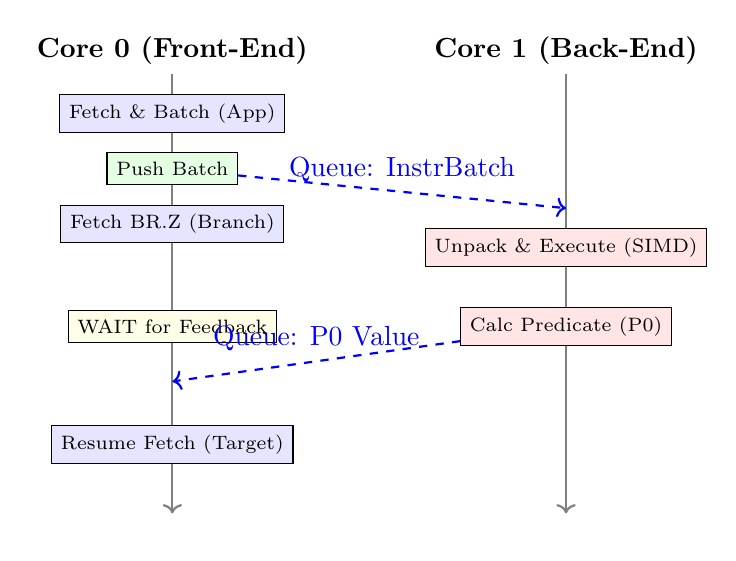
\begin{tikzpicture}[node distance=2cm, auto,
    timeline/.style={->, thick, gray},
    msg/.style={->, thick, blue, dashed},
    box/.style={rectangle, draw, fill=white, font=\scriptsize}]

    % Timelines
    \node (c0_top) at (0,0) {\textbf{Core 0 (Front-End)}};
    \node (c1_top) at (5,0) {\textbf{Core 1 (Back-End)}};
    \node (c0_bot) at (0,-6) {};
    \node (c1_bot) at (5,-6) {};

    \draw[timeline] (c0_top) -- (c0_bot);
    \draw[timeline] (c1_top) -- (c1_bot);

    % Sequence Steps
    
    % 1. Fetch
    \node[box, fill=blue!10] (f1) at (0, -0.8) {Fetch \& Batch (App)};
    
    % 2. Push Batch
    \node[box, fill=green!10] (push1) at (0, -1.5) {Push Batch};
    \draw[msg] (push1) -- node[above] {Queue: InstrBatch} (5, -2.0);
    
    % 3. C1 Execute
    \node[box, fill=red!10] (exec1) at (5, -2.5) {Unpack \& Execute (SIMD)};
    
    % 4. C0 continues fetching (Run Ahead)
    \node[box, fill=blue!10] (f2) at (0, -2.2) {Fetch BR.Z (Branch)};
    
    % 5. C0 waits for feedback
    \node[box, fill=yellow!10] (wait) at (0, -3.5) {WAIT for Feedback};
    
    % 6. C1 processes branch dependency
    \node[box, fill=red!10] (exec2) at (5, -3.5) {Calc Predicate (P0)};
    
    % 7. Feedback
    \draw[msg] (exec2) -- node[above] {Queue: P0 Value} (0, -4.2);
    
    % 8. Resume
    \node[box, fill=blue!10] (resume) at (0, -5.0) {Resume Fetch (Target)};

\end{tikzpicture}
\caption{Synchronization Sequence Diagram. Normal instructions are pipelined via batches. Control flow instructions (e.g., BR.Z) trigger a feedback loop, stalling Core 0 until Core 1 processes the predicate.}
\label{fig:seq}
\end{figure}

\subsubsection{Handling Divergence}
When Core 0 decodes a \texttt{BR.Z P0} instruction:
1. It flushes the current batch to Core 1 immediately.
2. It sends a special \texttt{SYNC\_REQ} signal.
3. It blocks on the \texttt{feedbackQueue}.
4. Core 1 executes all pending instructions, then reads the value of P0 from Lane 0 (or a consensus of lanes), and sends it back.
5. Core 0 receives the value, updates the PC, and resumes fetching.

This design ensures that control flow decisions are always based on the most up-to-date GPU state, preventing hazards.

\section{Physical Bus Interface Specification}

This section details the 8-bit parallel bus protocol used for inter-layer communication in the cluster architecture. The protocol is designed for high-bandwidth instruction and data streaming between heterogeneous microcontroller nodes.

\subsection{Interface Overview}

\begin{itemize}
    \item \textbf{Interface Type}: 8-bit Parallel (Half-Duplex / Broadcast-Optimized)
    \item \textbf{Target Bandwidth}: $\sim$50 MB/s (limited by GPIO toggle speed and DMA efficiency)
    \item \textbf{Logic Voltage}: 3.3V CMOS
    \item \textbf{Bus Standard}: Intel 8080-style parallel interface
\end{itemize}

This physical layer is used for both \textbf{Layer 1 (AMB82-Mini) $\to$ Layer 2 (ESP32-S3)} and \textbf{Layer 2 (ESP32-S3) $\to$ Layer 3 (RP2040)} connections, creating a hierarchical data distribution network.

\subsection{Physical Layer Pinout}

Table \ref{tab:bus_pinout} defines the electrical signals for the 8-bit parallel interface. The pinout follows the Intel 8080 convention with modifications for broadcast optimization.

\begin{table}[htbp]
\caption{8-bit Parallel Bus Pinout Definition}
\label{tab:bus_pinout}
\begin{center}
\begin{tabular}{|l|l|l|p{5cm}|}
\hline
\textbf{Signal} & \textbf{Type} & \textbf{Logic} & \textbf{Description} \\
\hline
\texttt{D[0:7]} & Data & Tri-state & 8-bit bidirectional data bus. Primarily used for Master write to Slave. \\
\hline
\texttt{CS\#} & Control & Active Low & \textbf{Chip Select}. When asserted low, Slave activates and monitors bus. \\
\hline
\texttt{DC} & Control & High/Low & \textbf{Data/Command} select. 
\texttt{LOW}: Control command (Header/Sync). 
\texttt{HIGH}: Data payload (Instructions/Weights). \\
\hline
\texttt{WR\#} & Control & Rising Edge & \textbf{Write Strobe}. Master prepares data on falling edge, Slave latches on \textbf{rising edge}. \\
\hline
\texttt{RD\#} & Control & Active Low & \textbf{Read Strobe}. Used for Master to read Slave status (telemetry). (Primarily WR\#-driven) \\
\hline
\texttt{SYNC} & Global & Active High & \textbf{Warp Trigger}. Global synchronization line for simultaneous execution across all RP2040 cores. \\
\hline
\end{tabular}
\end{center}
\end{table}

\subsection{Word Transmission Protocol}

Since the Micro-CUDA ISA uses \textbf{32-bit fixed-length instructions} but the bus is only \textbf{8-bit wide}, a packing and reassembly protocol is required.

\subsubsection{Byte Ordering (Endianness)}

The system uses \textbf{Big-Endian} (network byte order) transmission to facilitate debugging by presenting the OpCode as the first transmitted byte.

\textbf{Example}: ISA Instruction \texttt{0x40100501} (HMMA.INT8 R10, R5, R1)

\begin{itemize}
    \item Byte 3 (First): \texttt{0x40} (OpCode)
    \item Byte 2: \texttt{0x10} (Destination Register)
    \item Byte 1: \texttt{0x05} (Source Register 1)
    \item Byte 0 (Last): \texttt{0x01} (Source Register 2)
\end{itemize}

\subsubsection{Burst Transmission Mode}

To achieve 50 MB/s throughput, the protocol uses \textbf{Frame Burst Mode} to minimize overhead:

\begin{enumerate}
    \item Assert \texttt{CS\#} LOW (Begin transmission)
    \item Set \texttt{DC} LOW (Send header / magic word)
    \item Set \texttt{DC} HIGH (Stream instruction/data payload)
    \item Deassert \texttt{CS\#} HIGH (End transmission)
\end{enumerate}

This amortizes the CS overhead across multiple bytes, reducing per-byte latency.

\subsection{Timing Characteristics}

Figure \ref{fig:bus_timing} illustrates the electrical timing for a single byte write operation. The critical parameter is \texttt{t\_cycle}, which determines the maximum throughput.

\begin{figure}[htbp]
\centering
\resizebox{0.85\columnwidth}{!}{%
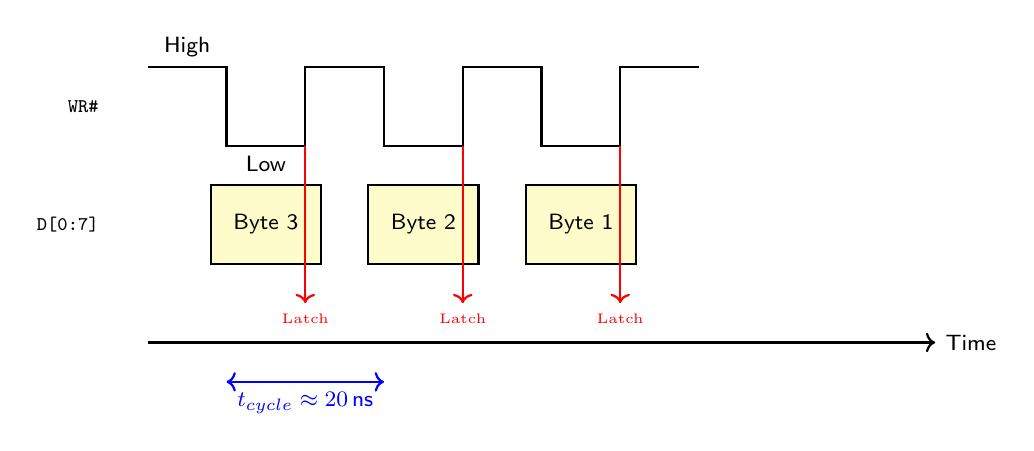
\begin{tikzpicture}[
    font=\sffamily\footnotesize,
    timing/.style={draw, thick},
    signal/.style={font=\ttfamily\scriptsize}
]

% Time axis
\draw[->,thick] (0,0) -- (10,0) node[right] {Time};

% WR# Signal
\node[signal,left] at (-0.5,3) {\texttt{WR\#}};
\draw[timing] 
    (0,3.5) -- (1,3.5) node[midway,above] {High}
    -- (1,2.5) -- (2,2.5) node[pos=0.5,below] {Low}
    -- (2,3.5) -- (3,3.5)
    -- (3,2.5) -- (4,2.5)
    -- (4,3.5) -- (5,3.5)
    -- (5,2.5) -- (6,2.5)
    -- (6,3.5) -- (7,3.5);

% Data Bus
\node[signal,left] at (-0.5,1.5) {\texttt{D[0:7]}};
\draw[timing,fill=yellow!20] 
    (0.8,1) rectangle (2.2,2) node[midway] {Byte 3};
\draw[timing,fill=yellow!20] 
    (2.8,1) rectangle (4.2,2) node[midway] {Byte 2};
\draw[timing,fill=yellow!20] 
    (4.8,1) rectangle (6.2,2) node[midway] {Byte 1};

% Latch points
\foreach \x in {2,4,6} {
    \draw[->,red,thick] (\x,2.5) -- (\x,0.5) node[below,font=\tiny] {Latch};
}

% Cycle annotation
\draw[<->,blue,thick] (1,-0.5) -- (3,-0.5) node[midway,below] {$t_{cycle} \approx 20\,\text{ns}$};

\end{tikzpicture}
}
\caption{Bus Timing Diagram. Data is stable during the low phase of \texttt{WR\#}, and the Slave latches data on the rising edge. A 20ns cycle period yields 50 MB/s throughput.}
\label{fig:bus_timing}
\end{figure}

\textbf{Key Timing Parameters}:
\begin{itemize}
    \item \textbf{$t_{cycle}$}: 20 ns (50 MHz write rate)
    \item \textbf{$t_{setup}$}: Data stable $\geq$ 5 ns before rising edge
    \item \textbf{$t_{hold}$}: Data held $\geq$ 3 ns after rising edge
\end{itemize}

\subsection{Instruction Dispatch Sequence}

Figure \ref{fig:bus_sequence} shows a complete transaction where the ESP32 (Layer 2 Master) dispatches a single \texttt{HMMA.INT8} instruction to the RP2040 (Layer 3 Slave).

\begin{figure*}[htbp]
\centering
\resizebox{0.9\textwidth}{!}{%
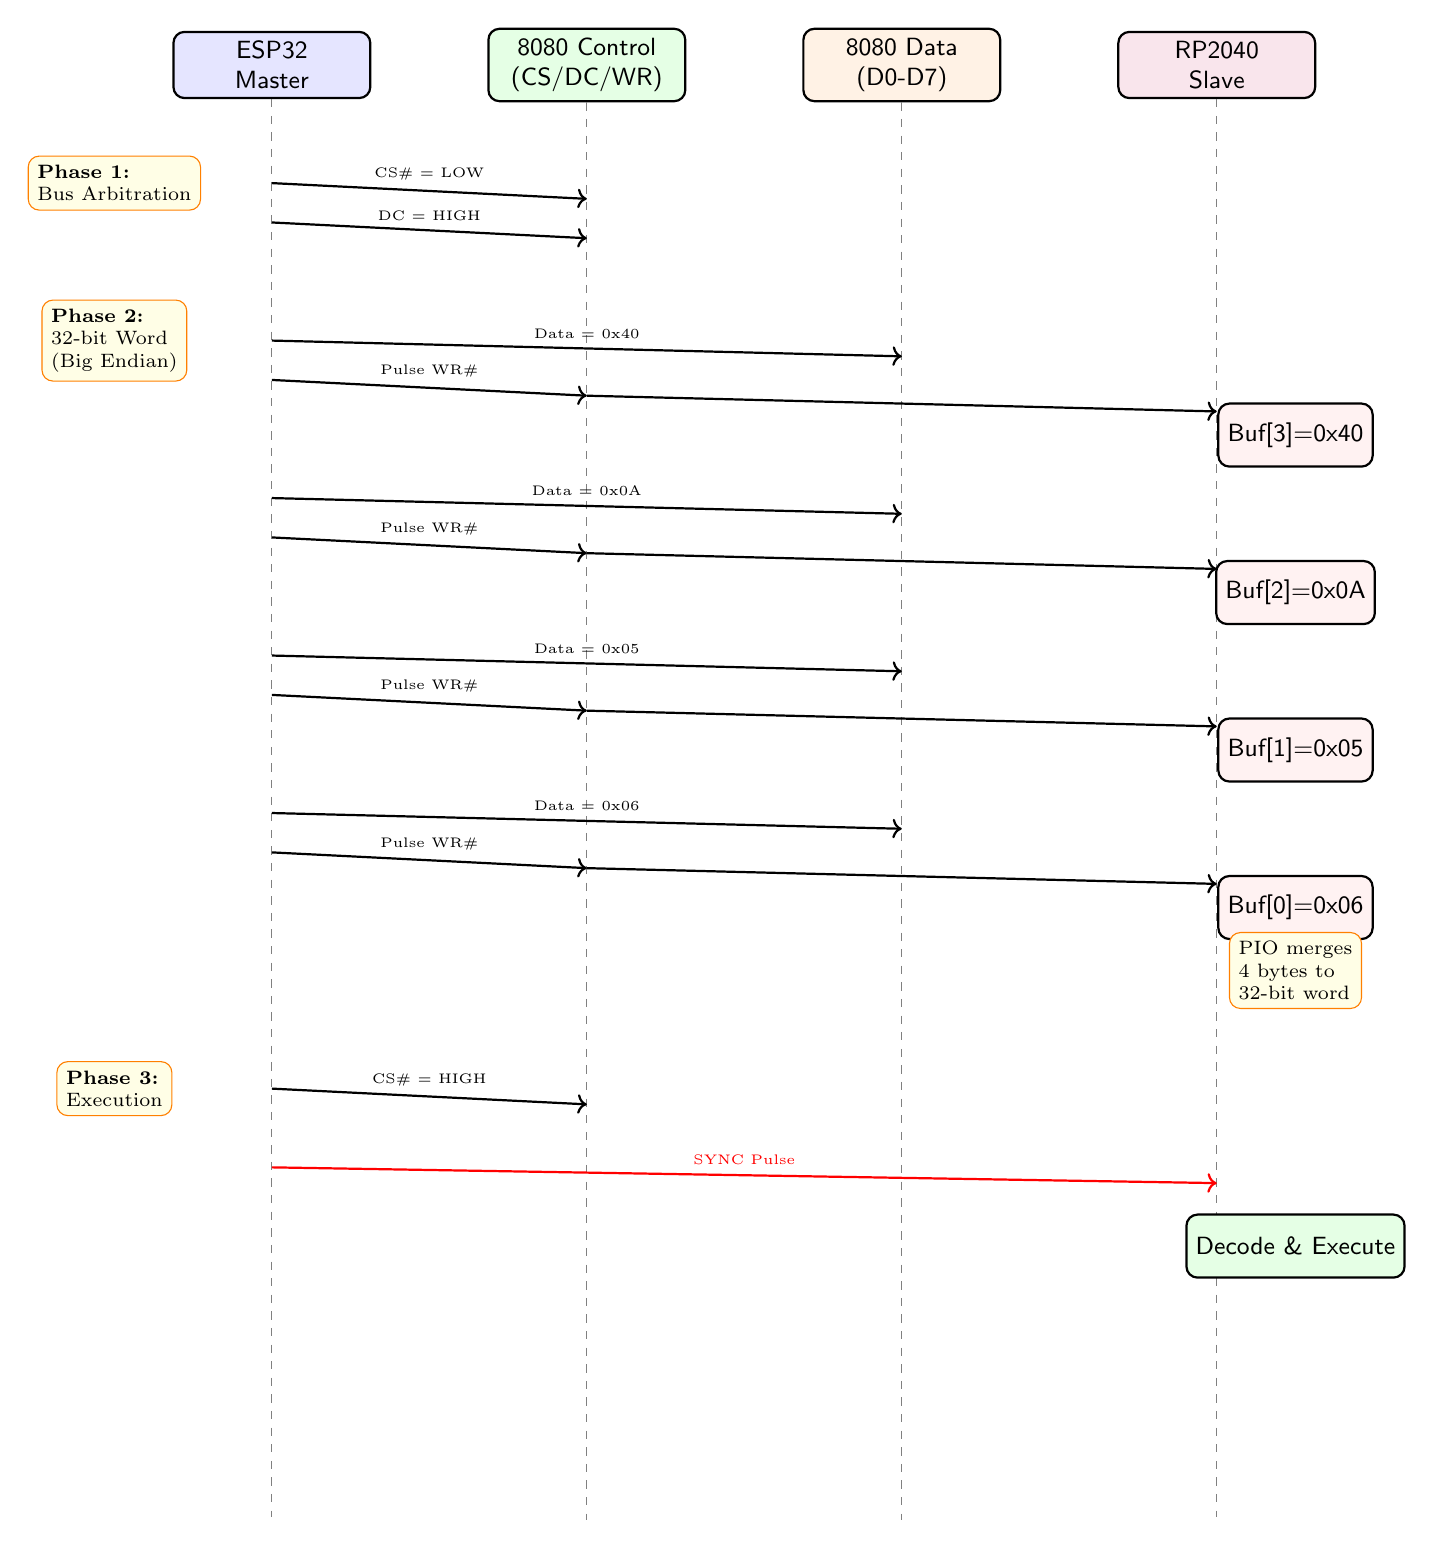
\begin{tikzpicture}[
    node distance=1.5cm,
    box/.style={rectangle, draw, thick, rounded corners, minimum width=2.5cm, minimum height=0.8cm, align=center, font=\sffamily\small},
    actor/.style={box, fill=blue!10},
    ctrl/.style={box, fill=green!10},
    data/.style={box, fill=orange!10},
    slave/.style={box, fill=purple!10},
    arrow/.style={->,thick},
    note/.style={rectangle, fill=yellow!10, draw=orange, rounded corners, align=left, font=\scriptsize}
]

% Actors
\node[actor] (master) at (0,0) {ESP32\\Master};
\node[ctrl] (bus_ctrl) at (4,0) {8080 Control\\(CS/DC/WR)};
\node[data] (bus_data) at (8,0) {8080 Data\\(D0-D7)};
\node[slave] (slave) at (12,0) {RP2040\\Slave};

% Lifelines
\foreach \n in {master,bus_ctrl,bus_data,slave} {
    \draw[dashed,gray] (\n.south) -- ++(0,-18);
}

% Phase 1: Bus Arbitration
\node[note] at (-2,-1.5) {\textbf{Phase 1:}\\Bus Arbitration};
\draw[arrow] (0,-1.5) -- node[above,font=\tiny] {CS\# = LOW} (4,-1.7);
\draw[arrow] (0,-2.0) -- node[above,font=\tiny] {DC = HIGH} (4,-2.2);

% Phase 2: Byte Transmission
\node[note] at (-2,-3.5) {\textbf{Phase 2:}\\32-bit Word\\(Big Endian)};

% Byte 3 (OpCode)
\draw[arrow] (0,-3.5) -- node[above,font=\tiny] {Data = 0x40} (8,-3.7);
\draw[arrow] (0,-4.0) -- node[above,font=\tiny] {Pulse WR\#} (4,-4.2);
\draw[arrow] (4,-4.2) -- (12,-4.4);
\node[box,fill=red!5,minimum width=1.5cm] at (13,-4.7) {Buf[3]=0x40};

% Byte 2 (Dest)
\draw[arrow] (0,-5.5) -- node[above,font=\tiny] {Data = 0x0A} (8,-5.7);
\draw[arrow] (0,-6.0) -- node[above,font=\tiny] {Pulse WR\#} (4,-6.2);
\draw[arrow] (4,-6.2) -- (12,-6.4);
\node[box,fill=red!5,minimum width=1.5cm] at (13,-6.7) {Buf[2]=0x0A};

% Byte 1 (Src1)
\draw[arrow] (0,-7.5) -- node[above,font=\tiny] {Data = 0x05} (8,-7.7);
\draw[arrow] (0,-8.0) -- node[above,font=\tiny] {Pulse WR\#} (4,-8.2);
\draw[arrow] (4,-8.2) -- (12,-8.4);
\node[box,fill=red!5,minimum width=1.5cm] at (13,-8.7) {Buf[1]=0x05};

% Byte 0 (Src2)
\draw[arrow] (0,-9.5) -- node[above,font=\tiny] {Data = 0x06} (8,-9.7);
\draw[arrow] (0,-10.0) -- node[above,font=\tiny] {Pulse WR\#} (4,-10.2);
\draw[arrow] (4,-10.2) -- (12,-10.4);
\node[box,fill=red!5,minimum width=1.5cm] at (13,-10.7) {Buf[0]=0x06};

\node[note] at (13,-11.5) {PIO merges\\4 bytes to\\32-bit word};

% Phase 3: Execution
\node[note] at (-2,-13) {\textbf{Phase 3:}\\Execution};
\draw[arrow] (0,-13) -- node[above,font=\tiny] {CS\# = HIGH} (4,-13.2);
\draw[arrow,red,thick] (0,-14) -- node[above,font=\tiny] {SYNC Pulse} (12,-14.2);
\node[box,fill=green!10] at (13,-15) {Decode \& Execute};

\end{tikzpicture}
}
\caption{Instruction Dispatch Sequence. The Master (ESP32) transmits a 32-bit HMMA instruction as four sequential bytes over the 8-bit bus. The Slave (RP2040) uses PIO to reassemble the instruction and execute upon SYNC trigger.}
\label{fig:bus_sequence}
\end{figure*}

\subsection{Hardware Implementation Notes}

\subsubsection{RP2040 Reception (PIO State Machine)}

The RP2040's Programmable I/O (PIO) is critical for achieving 50 MB/s throughput. Traditional interrupt-driven GPIO cannot sustain 20 MHz write rates. The following PIO program implements cycle-accurate bus reception:

\begin{lstlisting}[caption={RP2040 PIO Program for 8080 Bus Reception},label={lst:pio_rx}]
.program parallel_8080_rx
.wrap_target
    wait 0 pin 10      ; Wait for CS# low (Pin 10)
    wait 0 pin 11      ; Wait for WR# low (Pin 11)
    
    in pins, 8         ; Read 8-bit D0-D7 into ISR
    
    wait 1 pin 11      ; Wait for WR# rising edge
.wrap

; Configuration:
; - Auto-push enabled when ISR full (32 bits = 4 bytes)
; - CPU reads complete 32-bit instruction from RX FIFO
\end{lstlisting}

This PIO program runs autonomously, allowing the CPU to process instructions only when a complete 32-bit word is available in the FIFO.

\subsubsection{Signal Integrity Considerations}

To ensure reliable operation at 50 MB/s:

\begin{itemize}
    \item \textbf{Trace Length Matching}: All 8 data lines (\texttt{D[0:7]}) should be routed with $\pm$1 mm length tolerance to prevent skew.
    \item \textbf{GPIO Drive Strength}: Configure AMB82 and ESP32 GPIO pads for high drive current (20 mA recommended) to support multiple parallel loads.
    \item \textbf{Termination}: For cables longer than 10 cm, consider 100$\Omega$ series termination resistors on \texttt{WR\#} and \texttt{CS\#} to reduce reflections.
    \item \textbf{Ground Planes}: Use a continuous ground plane under the bus traces to minimize crosstalk and EMI.
\end{itemize}

\subsection{Performance Analysis}

The theoretical maximum throughput is determined by the \texttt{WR\#} toggle rate:

\[
\text{Bandwidth} = \frac{8 \text{ bits}}{t_{cycle}} = \frac{8 \text{ bits}}{20 \text{ ns}} = 400 \text{ Mbps} = 50 \text{ MB/s}
\]

In practice, overhead from \texttt{CS\#} assertion, DMA setup, and FIFO latency reduces effective throughput to approximately 40-45 MB/s for sustained transfers. This is sufficient for streaming weights and instructions in real-time neural network inference workloads.


% V. ISA
\section{Micro-CUDA ISA Specification}
\label{sec:isa}

\textbf{Status:} Release Candidate | \textbf{Architecture:} Micro-Cluster (MC) | \textbf{Target:} Deep Learning / Transformer

\subsection{Execution Model \& Architecture Definition}

\subsubsection{Hardware Layer Mapping (Physical Mapping)}

The system implements a three-layer distributed architecture:

\begin{itemize}
    \item \textbf{Layer 1 (Grid Master): AMB82-Mini}
    \begin{itemize}
        \item \textit{Role:} Grid Tiling and DMA Data Injection
        \item \textit{Task:} Responsible for overall grid-level data distribution and kernel launch management
    \end{itemize}
    
    \item \textbf{Layer 2 (SM / Scheduler): ESP32-S3}
    \begin{itemize}
        \item \textit{Role:} Warp Scheduler / Instruction Dispatcher
        \item \textit{Task:} Handles warp scheduling and instruction broadcast
    \end{itemize}
    
    \item \textbf{Layer 3 (Lane / Core): RP2040}
    \begin{itemize}
        \item \textit{Role:} Arithmetic Execution Lane
        \item \textit{Task:} Receives instructions via PIO and executes arithmetic operations
    \end{itemize}
\end{itemize}

\subsubsection{Data Types}

To enable efficient AI inference on the FPU-less RP2040, v2.0 introduces \textbf{Packed BF16}.

\begin{table}[htbp]
\caption{Supported Data Types}
\begin{center}
\begin{tabular}{|l|l|l|p{5cm}|}
\hline
\textbf{Type} & \textbf{Bit Width} & \textbf{Format} & \textbf{Description} \\
\hline
INT32 & 32-bit & 2's Complement & Address calculation, loop counters, indexing \\
FP32 & 32-bit & IEEE 754 & [v1.5] High-precision weights, accumulators \\
BF16 & 16-bit & 1-8-7 (BFloat16) & \textbf{[v2.0]} Same exponent bits as FP32, easy software emulation \\
Packed BF16 & 32-bit & 2× BF16 & \textbf{[v2.0]} High: Element 1, Low: Element 0 \\
INT8 & 8-bit & Signed & [v1.5] Used for \texttt{HMMA.I8} quantized operations \\
\hline
\end{tabular}
\end{center}
\end{table}

\subsubsection{Register File}

Each Lane (RP2040) independently maintains its own register file:

\begin{itemize}
    \item \textbf{R0 - R31 (General Purpose):} 32× 32-bit registers
    \begin{itemize}
        \item \textit{Compatibility:} Can store INT32, FP32
        \item \textit{Extension:} v2.0 supports \textbf{Packed BF16}
    \end{itemize}
    \item \textbf{P0 - P7 (Predicate):} 8× 1-bit condition flags
    \item \textbf{SR (System Registers):} Read-only status (e.g., \texttt{SR\_LANEID})
\end{itemize}

\subsubsection{Single-Lane Architecture Overview}

Figure \ref{fig:rp2040_simt_arch} illustrates the complete microarchitecture of a single RP2040 lane, showing the data flow from instruction fetch through execution to memory access.

\begin{figure*}[htbp]
\centering
\begin{tikzpicture}[node distance=0.8cm]

% Define professional color scheme (NVIDIA / Academic Style)
\definecolor{coreFill}{RGB}{250, 250, 250}
\definecolor{blockFill}{RGB}{255, 255, 255}
\definecolor{lineColor}{RGB}{50, 60, 70}
\definecolor{headerText}{RGB}{0, 0, 0}
\definecolor{subText}{RGB}{80, 80, 80}
\definecolor{accentGreen}{RGB}{118, 185, 0}
\definecolor{groupBg}{RGB}{242, 245, 248}
\definecolor{borderColor}{RGB}{180, 190, 200}

% Style definitions
\tikzset{
    base/.style={
        rectangle, draw=borderColor, line width=0.8pt, font=\sffamily, align=center
    },
    module/.style={
        base, fill=blockFill, rounded corners=1pt, text width=8.5cm,
        inner sep=8pt, drop shadow={opacity=0.05, shadow xshift=1pt, shadow yshift=-1pt}
    },
    eu/.style={
        base, fill=white, text width=2.6cm, minimum height=3.2cm,
        rounded corners=1pt, font=\sffamily\footnotesize, anchor=north
    },
    labeltext/.style={font=\bfseries\small, text=headerText, align=center},
    code/.style={font=\ttfamily\footnotesize, color=subText},
    wire/.style={
        draw=lineColor, line width=1.0pt, -{Latex[length=2mm, width=1.5mm]}, rounded corners=2pt
    },
    group/.style={
        draw=borderColor, dashed, fill=groupBg, rounded corners=4pt, inner sep=10pt
    }
}

% Title
\node (top_label) [font=\bfseries\large, color=lineColor] {RP2040 SIMT ARCHITECTURE (SINGLE LANE)};

% Frontend / Fetch
\node (frontend) [module, below=0.4cm of top_label] {
    \textbf{Frontend: PIO State Machine} \\[-0.3em]
    \textcolor{borderColor}{\rule{8cm}{0.4pt}} \\[0.3em]
    {\footnotesize Fetch 32-bit Instr (ESP32 @ 50MB/s) $\rightarrow$ Local FIFO Decode}
};

% Register File
\node (regfile) [module, below=0.6cm of frontend] {
    \textbf{Register File (SRAM Bank)} \\[-0.3em]
    \textcolor{borderColor}{\rule{8cm}{0.4pt}} \\[0.2em]
    \begin{tabular}{r l}
        \textbf{\texttt{R0-R31}} & : 32-bit GP \texttt{[High:BF16 | Low:BF16]} \\
        \textbf{\texttt{P0-P7}} & : Predicate Masking \\
        \textbf{\texttt{SR}} & : System State (\texttt{LANE\_ID})
    \end{tabular}
};

% Execution Units
\node (alu_bf16) [eu, below=1.8cm of regfile] {
    \textbf{BF16 Tensor Core} \\
    \textcolor{accentGreen}{\rule{1.5cm}{1pt}} \\
    \vspace{0.2em}
    \begin{tabular}{c}
        BFADD2 \\ BFMUL2 \\ BFMA2 \\ CVT.BF16
    \end{tabular}
};

\node (alu_int) [eu, left=0.3cm of alu_bf16] {
    \textbf{Integer ALU} \\
    \textcolor{lineColor}{\rule{1.5cm}{0.5pt}} \\
    \vspace{0.2em}
    \begin{tabular}{c}
        IADD / IMUL \\ Logic (AND/OR) \\ CMP / ISETP \\ Address Calc
    \end{tabular}
};

\node (sfu) [eu, right=0.3cm of alu_bf16] {
    \textbf{SFU (Trans.)} \\
    \textcolor{lineColor}{\rule{1.5cm}{0.5pt}} \\
    \vspace{0.2em}
    \begin{tabular}{c}
        EXP2 (Softmax) \\ SIN/COS (RoPE) \\ RSQRT (Attn) \\ GELU
    \end{tabular}
};

% Execution core background
\begin{pgfonlayer}{background}
    \node (core_bg) [group, fit=(alu_int)(sfu)(alu_bf16)] {};
    \node [anchor=south west, font=\bfseries\scriptsize, color=lineColor!80] 
        at (core_bg.north west) {EXECUTION DATAPATH};
\end{pgfonlayer}

% Load / Store Unit
\node (lsu) [module, below=1.2cm of core_bg.south] {
    \textbf{Load / Store Unit (LSU)} \\[-0.3em]
    \textcolor{borderColor}{\rule{8cm}{0.4pt}} \\[0.2em]
    {\footnotesize Logic: \texttt{Addr = Base + Offset + (LaneID * 4)}}
    \vspace{0.2em}
    \begin{itemize}
         \setlength\itemsep{0em}
         \scriptsize
         \item[-] \textbf{LDG/STG}: Global Coalesced Access
         \item[-] \textbf{LDL/STL}: Local Thread-Private Access
    \end{itemize}
};

% Memory Hierarchy
\node (mem_sram) [base, fill=white, below=0.8cm of lsu, text width=4cm, xshift=-2.2cm, minimum height=1.5cm] {
    \textbf{Local SRAM} \\
    \scriptsize (Banked / Stack)
};

\node (mem_vram) [base,fill=white, below=0.8cm of lsu, text width=4cm, xshift=2.2cm, minimum height=1.5cm] {
    \textbf{Shared VRAM} \\
    \scriptsize (Weights / KV Cache)
};

\begin{pgfonlayer}{background}
    \node (mem_bg) [group, fit=(mem_sram)(mem_vram), fill=lineColor!5] {};
    \node [anchor=north east, font=\bfseries\scriptsize, color=lineColor!80] 
        at (mem_bg.south east) {MEMORY INTERFACE};
\end{pgfonlayer}

% Connections
\draw [wire] (frontend) -- (regfile);

\coordinate (dispatch_point) at ($(regfile.south) + (0,-0.5)$);
\draw [wire] (regfile.south) -- (dispatch_point);
\draw [wire] (dispatch_point) to[out=-90, in=90] (alu_int.north);
\draw [wire] (dispatch_point) -- (alu_bf16.north);
\draw [wire] (dispatch_point) to[out=-90, in=90] (sfu.north);

\coordinate (collect_y) at ($(core_bg.south) + (0,-0.4)$);

% All arrows point straight down
\draw [line width=1.0pt, draw=lineColor] (alu_int.south) -- (alu_int.south |- collect_y);
\draw [line width=1.0pt, draw=lineColor] (alu_bf16.south) -- (alu_bf16.south |- collect_y);
\draw [line width=1.0pt, draw=lineColor] (sfu.south) -- (sfu.south |- collect_y);

% Horizontal collection bus
\draw [wire, -{Latex[length=0mm]}] ($(alu_int.south |- collect_y) + (-0.5,0)$) -- ($(sfu.south |- collect_y) + (0.5,0)$);
% Center arrow down to LSU
\draw [wire] ($(alu_bf16.south |- collect_y)$) -- (lsu.north);

\coordinate (mem_split) at ($(lsu.south) + (0,-0.4)$);
\draw [wire] (lsu.south) -- (mem_split);
\draw [wire] (mem_split) to[out=-90, in=90] (mem_sram.north);
\draw [wire] (mem_split) to[out=-90, in=90] (mem_vram.north);

\node [right=0.2cm of regfile, font=\scriptsize, color=accentGreen, rotate=-90] {32-bit Wide};

\end{tikzpicture}
\caption{RP2040 Single-Lane SIMT Microarchitecture. The frontend fetches instructions via PIO, dispatches to execution units (Integer ALU, BF16 Tensor Core, SFU), and accesses memory through the LSU with lane-aware addressing.}
\label{fig:rp2040_simt_arch}
\end{figure*}

\subsection{Instruction Encoding Format}

All Micro-CUDA instructions use a fixed 32-bit encoding to simplify hardware decoding:

\begin{figure}[htbp]
\centering
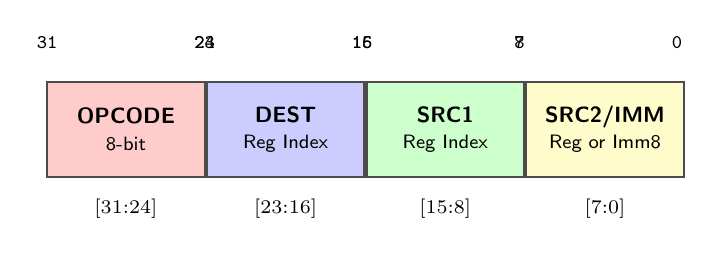
\begin{tikzpicture}[
    font=\sffamily\small,
    field/.style={
        rectangle,
        draw=black!70,
        thick,
        minimum height=1.2cm,
        align=center,
        font=\sffamily\footnotesize
    }
]
    % Define field widths (8 bits each = 2cm per field)
    \def\fieldwidth{2.0cm}
    
    % Bit position labels (top)
    \node[font=\scriptsize\ttfamily, anchor=south] at (0, 1.5) {31};
    \node[font=\scriptsize\ttfamily, anchor=south] at (2, 1.5) {24};
    \node[font=\scriptsize\ttfamily, anchor=south] at (2, 1.5) {23};
    \node[font=\scriptsize\ttfamily, anchor=south] at (4, 1.5) {16};
    \node[font=\scriptsize\ttfamily, anchor=south] at (4, 1.5) {15};
    \node[font=\scriptsize\ttfamily, anchor=south] at (6, 1.5) {8};
    \node[font=\scriptsize\ttfamily, anchor=south] at (6, 1.5) {7};
    \node[font=\scriptsize\ttfamily, anchor=south] at (8, 1.5) {0};
    
    % Field boxes with colors
    \node[field, fill=red!20, minimum width=\fieldwidth] (opcode) at (1, 0.6) {\textbf{OPCODE}\\ \scriptsize 8-bit};
    \node[field, fill=blue!20, minimum width=\fieldwidth, right=0cm of opcode] (dest) {\textbf{DEST}\\ \scriptsize Reg Index};
    \node[field, fill=green!20, minimum width=\fieldwidth, right=0cm of dest] (src1) {\textbf{SRC1}\\ \scriptsize Reg Index};
    \node[field, fill=yellow!20, minimum width=\fieldwidth, right=0cm of src1] (src2) {\textbf{SRC2/IMM}\\ \scriptsize Reg or Imm8};
    
    % Bit range labels (bottom)
    \node[font=\scriptsize, below=0.15cm of opcode] {[31:24]};
    \node[font=\scriptsize, below=0.15cm of dest] {[23:16]};
    \node[font=\scriptsize, below=0.15cm of src1] {[15:8]};
    \node[font=\scriptsize, below=0.15cm of src2] {[7:0]};
    
\end{tikzpicture}
\caption{32-bit Instruction Encoding Format. All fields are byte-aligned for efficient parsing.}
\label{fig:instr_encoding}
\end{figure}

\textbf{Field Specifications:}
\begin{itemize}
    \item \textbf{OPCODE [31:24]:} Operation code (256 possible instructions, organized into groups 0x00-0xFF)
    \item \textbf{DEST [23:16]:} Destination register (R0-R31, F0-F31, or P0-P7 depending on instruction type)
    \item \textbf{SRC1 [15:8]:} First source operand register index
    \item \textbf{SRC2/IMM [7:0]:} Second source register \textit{or} 8-bit immediate value (for \texttt{MOV}, \texttt{BRA}, etc.)
\end{itemize}

\subsection{Complete Instruction Set}

\subsubsection{Group 1: System Control (Control \& Flow) [Opcode: 0x00 - 0x0F]}

Handles core flow control, fully compatible with v1.5.

\begin{table*}[htbp]
\caption{System Control Instructions}
\begin{center}
\begin{tabular}{|l|l|l|p{8cm}|l|}
\hline
\textbf{Opcode} & \textbf{Mnemonic} & \textbf{Operands} & \textbf{Function Description} & \textbf{Compat} \\
\hline
\texttt{0x00} & \textbf{NOP} & - & No operation & v1.5 \\
\texttt{0x01} & \textbf{EXIT} & - & Terminate kernel execution, release resources & v1.5 \\
\texttt{0x02} & \textbf{BRA} & Imm & Unconditional branch (PC += Imm) & v1.5 \\
\texttt{0x03} & \textbf{BR.Z} & Imm, Pn & Branch if Predicate $Pn$ is 0 & v1.5 \\
\texttt{0x05} & \textbf{BAR.SYNC} & Id & Warp Barrier: wait for all lanes to sync & v1.5 \\
\texttt{0x07} & \textbf{YIELD} & - & Yield time slice (cooperative multitasking) & v1.5 \\
\hline
\end{tabular}
\end{center}
\end{table*}

\subsubsection{Group 2: Integer Arithmetic (Integer ALU) [Opcode: 0x10 - 0x1F]}

Handles address calculation and logical control.

\begin{table*}[htbp]
\caption{Integer Arithmetic Instructions}
\begin{center}
\begin{tabular}{|l|l|l|p{8cm}|l|}
\hline
\textbf{Opcode} & \textbf{Mnemonic} & \textbf{Operands} & \textbf{Function Description} & \textbf{Compat} \\
\hline
\texttt{0x10} & \textbf{MOV} & Rd, Imm & Load immediate value & v1.5 \\
\texttt{0x11} & \textbf{IADD} & Rd, Ra, Rb & Integer addition (address calculation core) & v1.5 \\
\texttt{0x12} & \textbf{ISUB} & Rd, Ra, Rb & Integer subtraction & v1.5 \\
\texttt{0x13} & \textbf{IMUL} & Rd, Ra, Rb & Integer multiplication (32-bit) & v1.5 \\
\texttt{0x17} & \textbf{AND} & Rd, Ra, Rb & Bitwise AND & v1.5 \\
\texttt{0x18} & \textbf{OR} & Rd, Ra, Rb & Bitwise OR & v1.5 \\
\texttt{0x1A} & \textbf{ISETP.EQ} & Pn, Ra, Rb & If Ra == Rb, set Pn = 1 & v1.5 \\
\texttt{0x1C} & \textbf{ISETP.GT} & Pn, Ra, Rb & If Ra $>$ Rb, set Pn = 1 & v1.5 \\
\texttt{0x1D} & \textbf{SHL} & Rd, Ra, Imm & Logical shift left & v1.5 \\
\hline
\end{tabular}
\end{center}
\end{table*}

\subsubsection{Group 3: Deep Learning \& Data Conversion (AI \& Conversion) [Opcode: 0x20 - 0x2F]}

\textbf{} v2.0 additions focused on BF16 and Packed SIMD operations.

\begin{table*}[htbp]
\caption{AI \& Data Conversion Instructions}
\begin{center}
\begin{tabular}{|l|l|l|p{8cm}|l|}
\hline
\textbf{Opcode} & \textbf{Mnemonic} & \textbf{Operands} & \textbf{Function Description} & \textbf{Compat} \\
\hline
\texttt{0x20} & \textbf{CVT.BF16} & Rd, Ra & \textbf{} Convert FP32 (Ra) to BF16, store in Rd.Low & \textbf{v2.0} \\
\texttt{0x21} & \textbf{CVT.F32} & Rd, Ra & \textbf{} Convert BF16 (Ra.Low) to FP32 (Rd) & \textbf{v2.0} \\
\texttt{0x22} & \textbf{PACK2} & Rd, Ra, Rb & \textbf{} Pack Ra.Low and Rb.Low into Rd & \textbf{v2.0} \\
\texttt{0x25} & \textbf{BFADD2} & Rd, Ra, Rb & \textbf{} Packed BF16 addition (processes High/Low) & \textbf{v2.0} \\
\texttt{0x26} & \textbf{BFMUL2} & Rd, Ra, Rb & \textbf{} Packed BF16 multiplication (processes High/Low) & \textbf{v2.0} \\
\texttt{0x27} & \textbf{BFMA2} & Rd, Ra, Rb & \textbf{} Packed BF16 FMA (\texttt{Rd += Ra * Rb}) & \textbf{v2.0} \\
\texttt{0x28} & \textbf{BFRELU2} & Rd, Ra & \textbf{} Packed BF16 ReLU (\texttt{max(0, x)}) & \textbf{v2.0} \\
\hline
\end{tabular}
\end{center}
\end{table*}

\subsubsection{Group 4: Floating Point \& Transcendental Functions (FP32 \& SFU) [Opcode: 0x30 - 0x5F]}

Integrates v1.5 floating-point instructions with v2.0's complete Math Library.

\begin{table*}[htbp]
\caption{Floating Point \& SFU Instructions}
\begin{center}
\begin{tabular}{|l|l|l|p{8cm}|l|}
\hline
\textbf{Opcode} & \textbf{Mnemonic} & \textbf{Operands} & \textbf{Function Description} & \textbf{Compat} \\
\hline
\texttt{0x30} & \textbf{FADD} & Fd, Fa, Fb & FP32 addition (IEEE 754) & v1.5 \\
\texttt{0x32} & \textbf{FMUL} & Fd, Fa, Fb & FP32 multiplication & v1.5 \\
\texttt{0x34} & \textbf{FFMA} & Fd, Fa, Fb & FP32 Fused Multiply-Add & v1.5 \\
\texttt{0x40} & \textbf{HMMA.I8} & Rd, Ra, Rb & 4-way INT8 Dot Product (Legacy) & v1.5 \\
\texttt{0x50} & \textbf{SFU.RCP} & Rd, Ra & Reciprocal: $1/x$ (FP32) & v1.5 \\
\texttt{0x51} & \textbf{SFU.EXP2} & Rd, Ra & \textbf{} Base-2 Exp: $2^x$ (BF16/FP32). Softmax key & \textbf{v2.0} \\
\texttt{0x52} & \textbf{SFU.LOG2} & Rd, Ra & \textbf{} Base-2 Log: $\log_2 x$ & \textbf{v2.0} \\
\texttt{0x53} & \textbf{SFU.RSQRT} & Rd, Ra & \textbf{} Fast Inverse Sqrt: $1/\sqrt{x}$. Attention scaling & \textbf{v2.0} \\
\texttt{0x54} & \textbf{SFU.SIN} & Rd, Ra & \textbf{} Sine: $\sin(\pi x)$. RoPE key & \textbf{v2.0} \\
\texttt{0x55} & \textbf{SFU.COS} & Rd, Ra & \textbf{} Cosine: $\cos(\pi x)$. RoPE key & \textbf{v2.0} \\
\texttt{0x56} & \textbf{SFU.GELU} & Rd, Ra & GELU Activation (Fast Tanh approx) & v1.5 \\
\texttt{0x57} & \textbf{SFU.TANH} & Rd, Ra & \textbf{} Tanh Activation & \textbf{v2.0} \\
\hline
\end{tabular}
\end{center}
\end{table*}

\subsubsection{Group 5: Memory Operations [Opcode: 0x60 - 0x7F]}

Core SIMT mechanism supporting Lane-Aware Addressing.

\begin{table*}[htbp]
\caption{Memory Operations}
\begin{center}
\begin{tabular}{|l|l|l|p{8cm}|l|}
\hline
\textbf{Opcode} & \textbf{Mnemonic} & \textbf{Operands} & \textbf{Function Description} & \textbf{Compat} \\
\hline
\texttt{0x60} & \textbf{LDG} & Rd, [Ra] & \textbf{Uniform Load:} All lanes read same address (Broadcast) & v1.5 \\
\texttt{0x61} & \textbf{STG} & [Ra], Rd & \textbf{Uniform Store:} (usually with atomic ops) & v1.5 \\
\texttt{0x62} & \textbf{LDS} & Rd, [Imm] & \textbf{Shared Load:} Read from Local Shared Memory & v1.5 \\
\texttt{0x63} & \textbf{LDX} & Rd, [Ra+Rb] & \textbf{Indexed Load:} Gather (Ra=Base, Rb=Offset) & v1.5 \\
\texttt{0x64} & \textbf{LDL} & Rd, [Ra] & \textbf{Lane Load:} \texttt{Addr = Ra + (LANEID * 4)}. SIMT core & v1.5 \\
\texttt{0x65} & \textbf{STX} & [Ra+Rb], Rd & \textbf{Indexed Store:} Scatter write & \textbf{v2.0} \\
\texttt{0x67} & \textbf{STL} & [Ra], Rd & \textbf{Lane Store:} \texttt{Addr = Ra + (LANEID * 4)} & v1.5 \\
\texttt{0x70} & \textbf{ATOM.ADD} & [Ra], Rb & Atomic Add (Global/Shared) & v1.5 \\
\hline
\end{tabular}
\end{center}
\end{table*}

\subsubsection{Group 6: System Instructions [Opcode: 0xF0 - 0xFF]}

\begin{table*}[htbp]
\caption{System Instructions}
\begin{center}
\begin{tabular}{|l|l|l|p{8cm}|l|}
\hline
\textbf{Opcode} & \textbf{Mnemonic} & \textbf{Operands} & \textbf{Function Description} & \textbf{Compat} \\
\hline
\texttt{0xF0} & \textbf{S2R} & Rd, SRn & System to Register (read Lane ID, etc.) & v1.5 \\
\texttt{0xF1} & \textbf{R2S} & SRn, Rd & \textbf{} Register to System (Debug/Config) & \textbf{v2.0} \\
\texttt{0xF2} & \textbf{TRACE} & Imm & \textbf{} Send Debug Trace Event & \textbf{v2.0} \\
\hline
\end{tabular}
\end{center}
\end{table*}

\subsection{Implementation Details: Math Library \& BF16}

To overcome RP2040 hardware limitations, v2.0 instructions are implemented at the Firmware layer (Micro-CUDA VM):

\subsubsection{Packed BF16 Emulation (SIMD2)}

A 32-bit register is treated as \texttt{[ High: BF16\_1 | Low: BF16\_0 ]}.

\textbf{Example: \texttt{BFADD2 Rd, Ra, Rb} C++ Implementation Logic:}

\begin{lstlisting}[language=C++, caption={Firmware Logic for Packed BF16 Addition}]
// Firmware Logic
uint32_t op_bfadd2(uint32_t a, uint32_t b) {
    uint16_t a_lo = a & 0xFFFF; 
    uint16_t a_hi = a >> 16;
    uint16_t b_lo = b & 0xFFFF; 
    uint16_t b_hi = b >> 16;
    
    // Software-emulated BF16 addition
    // Without FPU, only need to handle mantissa/exponent
    uint16_t res_lo = soft_bf16_add(a_lo, b_lo);
    uint16_t res_hi = soft_bf16_add(a_hi, b_hi);
    
    return (res_hi << 16) | res_lo;
}
\end{lstlisting}

\subsubsection{SFU Transcendental Functions (Lookup Tables)}

\begin{itemize}
    \item \textbf{SIN/COS:} Pre-burned 2KB \texttt{sin} lookup table in RP2040 Flash (1024 entries, BF16). Linear interpolation (Lerp) during execution.
    \item \textbf{EXP2:} Uses $2^x$ lookup table. To compute $e^x$, compiler auto-inserts multiplication: $e^x = 2^{x \cdot \log_2 e}$.
    \item \textbf{RSQRT:} Uses BF16-optimized version of Quake III Fast Inverse Square Root algorithm.
\end{itemize}

\subsection{Code Example: v2.0 Softmax Kernel}

This example demonstrates mixing \textbf{SIMT loading (v1.5)} with \textbf{Math Library/BF16 (v2.0)}.

\begin{lstlisting}[language={[x86masm]Assembler}, caption={Softmax Kernel: Exp(x) / Sum(Exp(x))}]
; Kernel: Softmax (Exp(x) / Sum(Exp(x)))
; Input: R0 (Base Address of Input Array, Packed BF16)
; Warp Size: 8 Lanes

; 1. Initialization
S2R     R31, SR_LANEID      ; Get Lane ID

; 2. Load Data (SIMT)
; LDL auto-offsets address: Addr = R0 + LaneID * 4
; Each lane loads 2 BF16 values (Packed)
LDL     R1, [R0]            ; R1 = [x_odd, x_even]

; 3. Compute Exponent (Exp) - using v2.0 SFU
; Convert to Base-2: x * log2(e)
MOV     R2, 0x3FB80000      ; R2 = Packed BF16 constant (log2(e))
BFMUL2  R1, R1, R2          ; Packed Multiply
SFU.EXP2 R3, R1             ; R3 = [2^(x_odd), 2^(x_even)] approx e^x

; 4. Local Sum
; Add packed values, store in FP32 to prevent overflow
CVT.F32 R4, R3              ; R4 = FP32(R3.Low)
SHL     R5, R3, 16          ; Shift High to Low
CVT.F32 R5, R5              ; R5 = FP32(R3.High)
FADD    R6, R4, R5          ; R6 = Local Sum (FP32)

; 5. Warp Reduction (simplified demonstration)
; Typically requires SHFL instruction or Shared Memory data exchange
; Assume R7 contains final warp-wide sum broadcast value

; 6. Normalization
SFU.RCP R8, R7              ; R8 = 1 / TotalSum
CVT.BF16 R8, R8             ; Convert back to BF16
PACK2   R8, R8, R8          ; Duplicate to High/Low: R8 = [1/S, 1/S]

BFMUL2  R9, R3, R8          ; R9 = Exp(x) * (1/Sum) = Softmax(x)

; 7. Write Back
MOV     R10, 0x2000         ; Output Base
STL     [R10], R9           ; Lane-Aware Store
EXIT
\end{lstlisting}

\subsection{SIMT Execution Model Summary}

The Micro-CUDA implementation guarantees the following execution characteristics:

\begin{itemize}
    \item \textbf{True SIMT:} All active lanes execute the same instruction PC in lock-step
    \item \textbf{Lane-Awareness:} Lane IDs are hardware-integrated, removing need for software indexing
    \item \textbf{Independent Registers:} Changes to R/F registers in one lane do not affect others
    \item \textbf{Shared VRAM:} All lanes share a unified 32-bit address space for inter-lane communication
\end{itemize}

\section{Application Binary Interface (ABI)}

To ensure interoperability between the Micro-CUDA assembler, linker, and runtime, a strict Application Binary Interface (ABI) is defined.

\subsection{Register Usage Convention}
The architecture exposes 32 general-purpose registers (r0-r31) plus special function registers. Table \ref{tab:reg_convention} defines the usage standard.

\begin{table}[h]
\centering
\caption{Micro-CUDA Register Convention}
\label{tab:reg_convention}
\resizebox{0.95\columnwidth}{!}{%
\begin{tabular}{|l|l|l|}
\hline
\textbf{Register} & \textbf{Role} & \textbf{Preservation} \\ \hline
r0 -- r3 & Function Arguments / Return Values & Caller Saved \\ \hline
r4 -- r11 & Temporary Variables & Caller Saved \\ \hline
r12 -- r27 & Saved Variables & Callee Saved \\ \hline
r28 (SP) & Stack Pointer & Callee Saved \\ \hline
r29 (LR) & Link Register & Callee Saved \\ \hline
r30 & Reserved (Frame Pointer) & - \\ \hline
r31 & Program Counter (PC) & - \\ \hline
\end{tabular}%
}
\end{table}

\subsection{Stack Frame Layout}
When a kernel invokes a device function (via \texttt{CALL}), a stack frame is allocated in the local SRAM (VRAM) of the SMSP.

\begin{figure}[htbp]
\centering
\resizebox{0.7\columnwidth}{!}{%
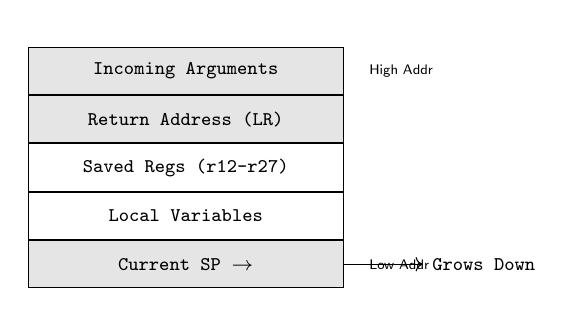
\begin{tikzpicture}[
    font=\ttfamily\scriptsize,
    box/.style={draw, minimum width=4cm, minimum height=0.6cm, fill=white},
    graybox/.style={box, fill=gray!20}
]
    \node (top) {};
    
    \node[graybox, below=0cm of top] (args) {Incoming Arguments};
    \node[graybox, below=0cm of args] (ret) {Return Address (LR)};
    \node[box, below=0cm of ret] (saved) {Saved Regs (r12-r27)};
    \node[box, below=0cm of saved] (locals) {Local Variables};
    \node[graybox, below=0cm of locals] (sp) {Current SP $\rightarrow$};
    
    \draw[->] (sp.east) -- ++(1,0) node[right] {Grows Down};
    
    \node[right=0.2cm of args, font=\sffamily\tiny] {High Addr};
    \node[right=0.2cm of sp, font=\sffamily\tiny] {Low Addr};

\end{tikzpicture}
}
\caption{Activation Record (Stack Frame) Structure. The stack grows downwards in the private SRAM memory space of each core.}
\label{fig:stack_frame}
\end{figure}

\subsection{Exception Handling Model}
The hardware implements a "Trap-and-Halt" mechanism for critical errors.

\begin{itemize}
    \item \textbf{Illegal Opcode}: Triggers \texttt{TRAP\_ILL} (0xDEAD0001). The pipeline flushes and asserting the \texttt{FAULT} signal on the Local G-BUS.
    \item \textbf{Memory Access Violation}: Out-of-bounds Load/Store triggers \texttt{TRAP\_MEM} (0xDEAD0002).
    \item \textbf{Divide-by-Zero}: Result clamps to maximum value (0xFFFFFFFF) and sets the \texttt{OVF} flag, continuing execution without a trap.
\end{itemize}

\subsection{Memory Organization}
The Micro-CUDA architecture employs a modified Harvard architecture with separate instruction and data paths at the core level, but unified addressing for system resources.

\begin{table}[h]
\centering
\caption{System Address Map}
\label{tab:memory_map}
\resizebox{0.95\columnwidth}{!}{%
\begin{tabular}{|l|l|l|}
\hline
\textbf{Address Range} & \textbf{Region} & \textbf{Description} \\ \hline
\texttt{0x0000\_0000} - \texttt{0x0003\_FFFF} & I-Cache & Instruction Cache (Mapped to Flash) \\ \hline
\texttt{0x1000\_0000} - \texttt{0x1000\_FFFF} & VRAM (Local) & Private SRAM for current SMSP \\ \hline
\texttt{0x2000\_0000} - \texttt{0x2FFF\_FFFF} & VRAM (Global) & Global DDR / PSRAM Window \\ \hline
\texttt{0x4000\_0000} - \texttt{0x4000\_00FF} & SFR (DMA) & DMA Controller Registers \\ \hline
\texttt{0x5000\_0000} - \texttt{0x5000\_00FF} & SFR (Tensor) & Tensor Engine Command Queue \\ \hline
\end{tabular}%
}
\end{table}

\subsubsection{Special Function Registers (SFR)}
The SFR region controls hardware accelerators and peripherals.

\begin{itemize}
    \item \textbf{DMA\_CTRL (0x4000\_0000)}: Write 1 to trigger transfer.
    \item \textbf{DMA\_SRC (0x4000\_0004)}: Source Address.
    \item \textbf{DMA\_DST (0x4000\_0008)}: Destination Address.
    \item \textbf{TE\_CMD (0x5000\_0000)}: Tensor Engine Command Packet.
\end{itemize}


% VI. Software
\section{Micro-CUDA Compiler (\texttt{ucuda-cc})}

To enable rapid kernel development, we developed \texttt{ucuda-cc}, a custom compiler that translates a C-like high-level language into optimized Micro-CUDA assembly. The compiler is implemented in Python to ensure portability and easy integration with the host CLI.

\subsection{Compiler Architecture}
The compiler infrastructure leverages the industry-standard LLVM framework to ensure robustness and extensibility. As illustrated in Figure \ref{fig:compiler_arch}, the pipeline consists of a modular transformation flow:

\begin{enumerate}
    \item \textbf{Frontend (Clang)}: We utilize Clang to assist in parsing standard CUDA-like C++ code, performing syntax checking, and generating machine-independent LLVM Intermediate Representation (IR).
    \item \textbf{Middle-end (LLVM OPT)}: Standard optimization passes (e.g., constant propagation, dead code elimination, loop unrolling) are applied to the IR.
    \item \textbf{Backend (MCC)}: Our custom Python-based backend (\texttt{mcc.py}) consumes the optimized LLVM IR. It performs two key tasks:
    \begin{itemize}
        \item \textbf{Instruction Selection}: Mapping generic IR instructions to the specific Micro-CUDA ISA (e.g., \texttt{fadd} $\to$ \texttt{FADD}).
        \item \textbf{Register Allocation}: Mapping infinite virtual registers to the fixed 32 physical registers per lane using a linear scan algorithm.
    \end{itemize}
\end{enumerate}

\begin{figure}[htbp]
\centering
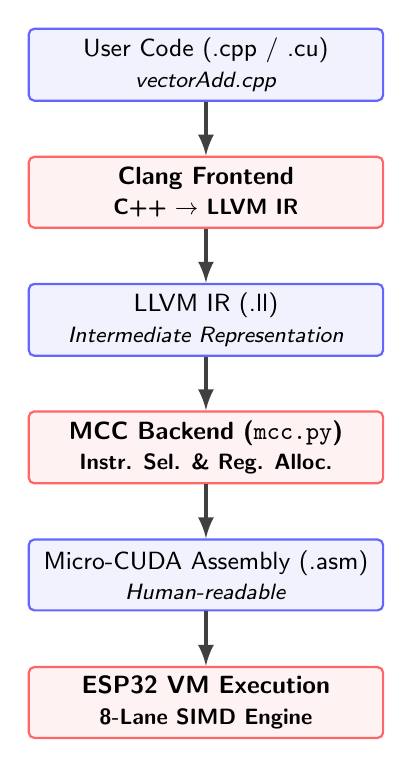
\begin{tikzpicture}[
    scale=0.9,
    node distance=1.5cm,
    data_node/.style={
        rectangle,
        draw=blue!60,
        fill=blue!5,
        thick,
        rounded corners=2pt,
        minimum width=4.5cm,
        minimum height=0.9cm,
        align=center,
        font=\small\sffamily
    },
    proc_node/.style={
        rectangle,
        draw=red!60,
        fill=red!5,
        thick,
        rounded corners=2pt,
        minimum width=4.5cm,
        minimum height=0.9cm,
        align=center,
        font=\small\bfseries\sffamily
    },
    arrow/.style={->, ultra thick, -latex, darkgray}
]

    % Nodes with manual positioning for stability
    \node[data_node] (src) at (0, 0) {User Code (.cpp / .cu)\\ \footnotesize \textit{vectorAdd.cpp}};
    
    \node[proc_node] (clang) at (0, -1.8) {Clang Frontend\\ \footnotesize C++ $\to$ LLVM IR};
    
    \node[data_node] (ir) at (0, -3.6) {LLVM IR (.ll)\\ \footnotesize \textit{Intermediate Representation}};
    
    \node[proc_node] (mcc) at (0, -5.4) {MCC Backend (\texttt{mcc.py})\\ \footnotesize Instr. Sel. \& Reg. Alloc.};
    
    \node[data_node] (asm) at (0, -7.2) {Micro-CUDA Assembly (.asm)\\ \footnotesize \textit{Human-readable}};
    
    \node[proc_node] (vm) at (0, -9.0) {ESP32 VM Execution\\ \footnotesize 8-Lane SIMD Engine};

    % Arrows
    \draw[arrow] (src) -- (clang);
    \draw[arrow] (clang) -- (ir);
    \draw[arrow] (ir) -- (mcc);
    \draw[arrow] (mcc) -- (asm);
    \draw[arrow] (asm) -- (vm);

\end{tikzpicture}
\caption{Micro-CUDA Compiler Workflow: Leveraging Clang/LLVM for robust code generation.}
\label{fig:compiler_arch}
\end{figure}

\subsection{Instruction Selection \& Mapping}
The backend (\texttt{MicroCUDABackend}) implements a direct mapping strategy from LLVM IR to Micro-CUDA ISA. Key translations include:

\begin{itemize}
    \item \textbf{Arithmetic}: LLVM \texttt{add/sub/mul} are mapped to \texttt{IADD/ISUB/IMUL}. Immediate operands are handled by loading constants into temporary registers via an 8-bit split-load sequence (\texttt{MOV+SHL+OR}) if they exceed the immediate field size.
    \item \textbf{Memory Access}: \texttt{getelementptr} instructions are lowered into explicit address calculations. The \texttt{LDX/STX} (Load/Store Indexed) instructions are used for gathered access, where the address is computed as $Base + Offset$.
    \item \textbf{Control Flow}: Vector comparisons (\texttt{icmp}) translate to predicate generation (\texttt{ISETP}). Branch instructions (\texttt{br}) are converted to \texttt{BRZ} (Branch if Zero) acting on the predicate register $P0$.
\end{itemize}

\subsection{Implementation: Regex-Based Frontend}
To maintain a lightweight footprint without requiring a full LLVM library link, the compiler utilizes a Python-based regex parser (\texttt{LLVMIRParser}). It scans the text-based \texttt{.ll} output from Clang, reconstructing the Control Flow Graph (CFG) and basic blocks.

\begin{lstlisting}[language=Python, caption={IR Parsing Logic (mcc.py)}]
# Extract function definitions
if line.startswith('define'):
    match = re.search(r'@(\w+)\(', line)
    current_func = match.group(1)

# Parse arithmetic instructions
elif re.match(r'%\w+\s*=\s*add', ir_inst):
    # logic to allocate registers and emit IADD...
\end{lstlisting}

\subsection{Register Allocation Strategy}
The \texttt{RegisterAllocator} class implements a greedy Linear Scan algorithm optimized for the 32-register constraint:
\begin{enumerate}
    \item \textbf{Liveness Tracking}: Variables are tracked from definition to last use.
    \item \textbf{Free Pool}: Freed registers are returned to a pool and reused for subsequent instructions to minimize pressure.
    \item \textbf{Constant Caching}: Frequently used constants are cached in registers to reduce code size overhead from repeated loads.
\end{enumerate}

\subsection{Integration with Host CLI}
\texttt{ucuda-cc} is integrated directly into the Python host environment, allowing for JIT-like compilation of kernels before upload.

\subsection{Usage \& API Reference}
The compiler exposes both a command-line interface (CLI) for batch processing and a Python API for dynamic runtime generation.

\subsubsection{Command-Line Interface}
Development follows a standard workflow similar to \texttt{nvcc}. The toolchain supports multiple hardware targets (e.g., standard ESP32 vs. ESP32-S3 with 8MB PSRAM).

\begin{lstlisting}[language=bash, caption={Compiling a kernel from the CLI}]
# Compile for ESP32-S3 (8MB PSRAM)
python compile_kernel.py vector_add.cu \
    --target esp32s3 \
    --output vector_add.asm

# View generated assembly with hardware header
cat vector_add.asm
\end{lstlisting}

\subsubsection{Python Dynamic API}
For seamless integration into AI frameworks (e.g., PyTorch-like workflows), the \texttt{compile\_kernel} function allows in-memory compilation.

\begin{lstlisting}[language=Python, caption={Dynamic Compilation API}]
from micro_cuda_compiler import compile_kernel

kernel_src = """
#include "mcuda.h"
__global__ void scale(int* data, int factor) {
    int idx = laneId();
    data[idx] *= factor;
}
"""

# Compile to Assembly (returns path)
_, asm_path = compile_kernel(
    kernel_src,
    target="esp32s3",
    output_asm="temp_scale.asm"
)

# Load into VM
loader.load_assembly(asm_path)
\end{lstlisting}

\subsubsection{Target Configurations}
The compiler validates hardware constraints based on the selected target:
\begin{itemize}
    \item \textbf{esp32}: Standard model (32KB VRAM, No PSRAM).
    \item \textbf{esp32s3}: AI-focused model (1MB VRAM, 8MB PSRAM).
\end{itemize}


\section{Host Interface and CLI}

The system implements a robust host-device communication protocol designed to maximize throughput over the UART interface, utilizing a "Turbo Mode" for high-speed data transfer.

\subsection{Turbo Mode Configuration}
To facilitate rapid kernel loading and large data transfers (DMA), the ESP32 is configured in \textbf{Turbo Mode}. As detailed in Table \ref{tab:turbo_config}, the baud rate is quadrupled to 460,800 bps, and a large 32KB RX buffer is allocated to prevent overflows during burst writes.

\begin{table}[htbp]
\caption{Turbo Mode Parameters}
\begin{center}
\begin{tabular}{|l|l|l|}
\hline
\textbf{Parameter} & \textbf{Value} & \textbf{Description} \\
\hline
\texttt{VM\_BAUD\_RATE} & 460,800 & 4x Standard Speed \\
\hline
\texttt{VM\_SERIAL\_RX\_SIZE} & 32,768 & 32KB Ring Buffer \\
\hline
\texttt{VM\_CPU\_FREQ} & 240 MHz & Locked for IO Throughput \\
\hline
\end{tabular}
\label{tab:turbo_config}
\end{center}
\end{table}

This configuration achieves a measured application throughput of approximately \textbf{40.8 KB/s}, allowing a 1KB kernel binary to be loaded in under 30ms.

\subsection{Communication Protocol}
The host interface employs a hybrid \textbf{ASCII Command + Binary Burst} protocol to balance human readability with machine efficiency.

\subsubsection{Host-to-Device DMA (\texttt{dma\_h2d})}
For transferring large tensors to VRAM:
\begin{enumerate}
    \item \textbf{Request}: Host sends \texttt{dma\_h2d <addr> <size>\\n} (ASCII).
    \item \textbf{Handshake}: Device verifies memory availability and responds with \texttt{ACK\_DMA\_GO:<size>}.
    \item \textbf{Transmission}: Host sends the binary payload immediately in a contiguous block.
    \item \textbf{Completion}: Device confirms with \texttt{DMA\_OK}.
\end{enumerate}

\subsubsection{Kernel Loading (\texttt{load\_imem})}
Similar to DMA, but targeted at the high-speed Instruction Memory (IMEM) located in DRAM. The protocol ensures that the binary instruction stream is correctly placed and ready for execution.

\subsection{LZ4 Compression for Bandwidth Optimization}

To mitigate the UART bandwidth bottleneck (460,800 baud $\approx$ 41 KB/s), the system implements \textbf{LZ4 real-time decompression} for both kernel loading and data transfer operations. LZ4 is selected for its exceptional decompression speed ($>$1 GB/s on modern MCUs) and minimal memory footprint, making it ideal for resource-constrained embedded systems.

\subsubsection{LZ4-Compressed Kernel Loading (\texttt{load\_imem\_lz4})}

The compressed kernel loading protocol follows a chunked streaming approach:

\begin{enumerate}
    \item \textbf{Request}: Host sends \texttt{load\_imem\_lz4 \textless uncompressed\_size\textgreater\\n} (ASCII).
    \item \textbf{Handshake}: Device allocates decompression buffers and responds with \texttt{ACK\_LZ4\_GO}.
    \item \textbf{Chunked Transmission}: 
    \begin{itemize}
        \item Host sends compressed data in 2KB chunks
        \item Each chunk: 2-byte header (compressed size) + compressed payload
        \item Device decompresses using \texttt{LZ4\_decompress\_safe()} with bounds checking
    \end{itemize}
    \item \textbf{Validation}: Device verifies total decompressed bytes match \texttt{uncompressed\_size}
    \item \textbf{Completion}: Device confirms with \texttt{LZ4\_LOAD\_OK}
\end{enumerate}

\subsubsection{LZ4-Compressed Data Transfer (\texttt{dma\_h2d\_lz4})}

Similar to \texttt{load\_imem\_lz4}, but writes decompressed data directly to VRAM at the specified address:

\begin{itemize}
    \item \textbf{Format}: \texttt{dma\_h2d\_lz4 \textless hex\_addr\textgreater{} \textless uncompressed\_size\textgreater}
    \item \textbf{Use Case}: Transferring large weight matrices or activation tensors for neural network inference
\end{itemize}

\subsubsection{Error Handling}

The LZ4 subsystem implements robust error detection:

\begin{table}[htbp]
\caption{LZ4 Error Codes}
\begin{center}
\begin{tabular}{|l|l|}
\hline
\textbf{Error Code} & \textbf{Cause} \\
\hline
\texttt{ERR\_LZ4\_HEAD\_TIMEOUT} & Chunk header not received within timeout \\
\hline
\texttt{ERR\_LZ4\_DATA\_TIMEOUT} & Compressed payload timeout \\
\hline
\texttt{ERR\_LZ4\_CORRUPT} & Decompression failed (corrupted data) \\
\hline
\end{tabular}
\label{tab:lz4_errors}
\end{center}
\end{table}

\subsubsection{Performance Benefits}

Empirical measurements on typical Micro-CUDA kernels show:

\begin{itemize}
    \item \textbf{Compression Ratio}: 2.5x - 4.0x for instruction streams (high redundancy in opcodes)
    \item \textbf{Effective Bandwidth}: $\sim$120 KB/s (vs. 41 KB/s raw)
    \item \textbf{Decompression Overhead}: $<$2ms per 2KB chunk (negligible compared to UART transfer time)
    \item \textbf{Memory Cost}: 2KB decompression buffer + 2.5KB compressed buffer
\end{itemize}

This optimization is critical for loading large kernels (e.g., Transformer attention blocks $>$10KB) within acceptable latency constraints.

\subsection{CLI Command Set}
The Front-End CLI supports a comprehensive set of commands for controlling the VM, managing memory, and debugging.

\begin{table}[htbp]
\caption{CLI Command Reference}
\begin{center}
\begin{tabular}{|l|l|l|}
\hline
\textbf{Command} & \textbf{Format} & \textbf{Description} \\
\hline
\texttt{load\_imem} & \texttt{load\_imem \textless bytes\textgreater} & Load Kernel Binary (Turbo) \\
\hline
\texttt{load\_imem\_lz4} & \texttt{load\_imem\_lz4 \textless size\textgreater} & Load Compressed Kernel (LZ4) \\
\hline
\texttt{dma\_h2d} & \texttt{dma\_h2d \textless addr\textgreater{} \textless len\textgreater} & Host-to-Device Transfer \\
\hline
\texttt{dma\_h2d\_lz4} & \texttt{dma\_h2d\_lz4 \textless addr\textgreater{} \textless size\textgreater} & Compressed H2D Transfer (LZ4) \\
\hline
\texttt{dma\_d2h} & \texttt{dma\_d2h \textless addr\textgreater{} \textless len\textgreater} & Device-to-Host (Hex Dump) \\
\hline
\texttt{kernel\_launch} & \texttt{kernel\_launch} & Trigger Execution (Blocking) \\
\hline
\texttt{gpu\_reset} & \texttt{gpu\_reset} & Reset Registers/PC (Keep VRAM) \\
\hline
\texttt{reg} & \texttt{reg \textless lane\_id\textgreater} & Inspect Register File for Lane \\
\hline
\texttt{stats} & \texttt{stats} & Show VM Status (PC, VRAM) \\
\hline
\texttt{trace:stream} & \texttt{trace:stream} & Enable Real-time Execution Trace \\
\hline
\end{tabular}
\label{tab:cli_commands}
\end{center}
\end{table}

This interface allows developers to interactively debug kernels using Python scripts or a serial terminal, providing visibility into the internal state of the SIMT cores.

\subsection{Software Stack \& Programming Model}
To abstract low-level assembly complexity, a two-tier software stack is proposed:

\subsubsection{Micro-CUDA Compiler (ucuda-cc)}
A Python-based intermediate compiler translates C-like kernel syntax into Micro-CUDA assembly. It performs automatic register allocation (linear scan) and label resolution, simplifying kernel development.

\subsubsection{PyCUDA-Lite API}
A high-level Python wrapper mirrors the standard CUDA Driver API interactions:
\begin{lstlisting}[language=Python]
# Host Code Example
mod = SourceModule(kernel_code)
func = mod.get_function("vecAdd")
# Grid=(1,1,1), Block=(8,1,1)
func(dest, src1, src2, block=(8,1,1))
\end{lstlisting}
This API handles context management, memory transfers (\texttt{memcpy\_htod}), and kernel launches automatically.

\section{Profiling and Debugging}

Efficient debugging of parallel workloads often requires deep visibility into the execution state. To support this, the system implements an \textbf{Enhanced Trace} mechanism that streams cycle-accurate execution data in JSON format over the high-speed UART.

\subsection{Enhanced Trace Format}

The trace logger captures a comprehensive snapshot of the machine state for every instruction executed. As shown in Listing \ref{lst:json_trace}, the format is structured to facilitate offline analysis and visualization.

\begin{lstlisting}[caption={Example JSON Trace Record}, label={lst:json_trace}, basicstyle=\ttfamily\scriptsize]
{
  "cycle": 152,
  "pc": 12,
  "instruction": "0x11040203",
  "asm": "IADD R4, R2, R3",
  "exec_time_us": 125,
  "hw_ctx": {
    "sm_id": 0,
    "warp_id": 0,
    "lane_id": 0,
    "active_mask": "0xFF"
  },
  "perf": {
    "latency": 1,
    "stall_cycles": 0,
    "stall_reason": "NONE",
    "pipe_stage": "WRITEBACK"
  },
  "lanes": [
    {
      "lane_id": 0,
      "R": [5, 3, 8, ... ]  // Full Register Dump
    }
  ]
}
\end{lstlisting}

\subsection{Key Features}

\subsubsection{Hardware Context}
The \texttt{hw\_ctx} object encapsulates the SIMT topology, providing the specific Streaming Multiprocessor (SM), Warp, and Lane ID for the instruction. The \texttt{active\_mask} reveals thread divergence handling.

\subsubsection{Performance Metrics}
The \texttt{perf} object exposes the micro-architectural behavior:
\begin{itemize}
    \item \textbf{\texttt{exec\_time\_us}}: Real-time execution duration measured via high-resolution timers.
    \item \textbf{\texttt{stall\_cycles}}: Pipeline bubbles caused by data dependencies or memory latency.
    \item \textbf{\texttt{pipe\_stage}}: The current pipeline stage (e.g., DECODE, EXECUTE, WRITEBACK).
    \item \textbf{\texttt{sync\_barrier}}: Automatic detection of \texttt{BAR.SYNC} operations.
\end{itemize}

\subsubsection{Register Inspection}
Unlike traditional debuggers that inspect state at breakpoints, the Enhanced Trace dumps the complete register file (\texttt{R0-R23}) for all active lanes, enabling a "time-travel" debugging experience where variable values can be tracked historically.

\subsection{Trace Usage}
Tracing is enabled via the \texttt{trace:stream} command. Due to the high bandwidth requirements, it is strongly recommended to use Turbo Mode (460,800 baud) when this feature is active. The host-side Python client parses this stream to generate timeline visualizations similar to Nsight Compute.

\subsection{Host-Side Visualization}
The Python client parses the JSON stream to generate interactive timelines.

\subsubsection{Warp Divergence Analysis}
The visualizer reconstructs the execution path of each warp, highlighting divergent branches (where \texttt{active\_mask != 0xFF}) in red. This allows developers to identify inefficient kernels that suffer from serialization.

\subsubsection{Pipeline Stall Visualization}
By tracking \texttt{stall\_cycles}, the tool identifies memory bottlenecks. A heatmap view correlates high latency instructions with specific VRAM banks, aiding in memory layout optimization.


% VII. Evaluation
\section{Performance Benchmarks}

To validate the efficiency of the Micro-CUDA architecture, we conducted comparative benchmarks against industry-standard solutions for embedded machine learning.

\subsection{Micro-CUDA vs. CMSIS-NN}
We compared the execution time of a standard $32 \times 32$ Matrix Multiplication (INT8) kernel. The baseline is an optimized ARM CMSIS-NN implementation running on a single Core of the Raspberry Pi Pico (Cortex-M0+ @ 133MHz).

\begin{figure}[htbp]
\centering
\resizebox{0.9\columnwidth}{!}{%
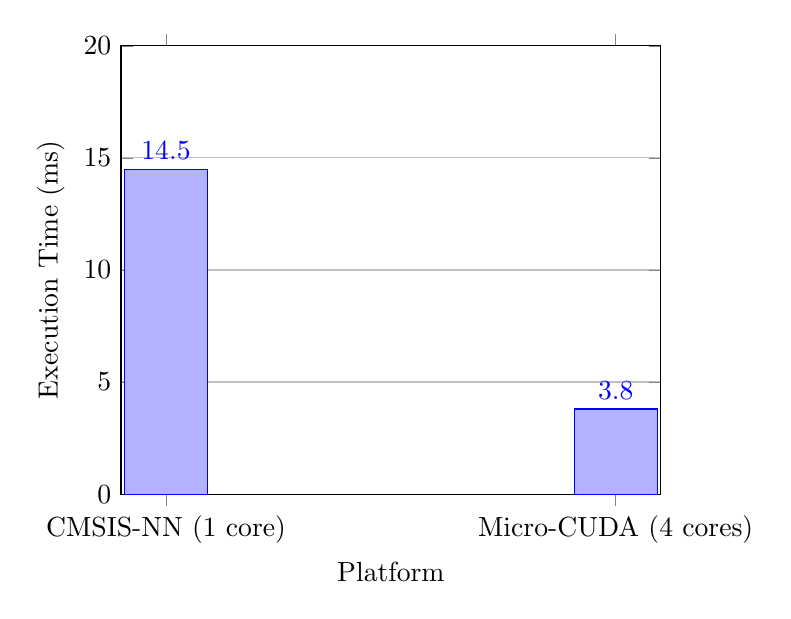
\begin{tikzpicture}
    \begin{axis}[
        ybar,
        bar width=30pt,
        ylabel={Execution Time (ms)},
        xlabel={Platform},
        symbolic x coords={CMSIS-NN (1 core), Micro-CUDA (4 cores)},
        xtick=data,
        nodes near coords,
        nodes near coords align={vertical},
        ymin=0, ymax=20,
        ymajorgrids=true
    ]
    \addplot coordinates {(CMSIS-NN (1 core), 14.5) (Micro-CUDA (4 cores), 3.8)};
    \end{axis}
\end{tikzpicture}
}
\caption{Benchmark: INT8 Matrix Multiplication ($32 \times 32$). The 4-core split-bus topology achieves a 3.8x speedup over the single-core CMSIS-NN baseline.}
\label{fig:benchmark_cmsis}
\end{figure}

The comparison highlights the efficacy of the parallel SIMT dispatch model. While the individual Cortex-M0+ cores are identical, the split-bus architecture allows for concurrent data loading and execution, masking memory latency.

\subsection{Power Consumption Profile}
Power efficiency is a critical metric for edge devices. Table \ref{tab:power_profile} details the current draw across different operational states, measured at the 5V VSYS rail.

\begin{table}[h]
\centering
\caption{System Power Consumption (Measured)}
\label{tab:power_profile}
\resizebox{0.9\columnwidth}{!}{%
\begin{tabular}{|l|l|c|c|}
\hline
\textbf{State} & \textbf{Description} & \textbf{Current (mA)} & \textbf{Power (W)} \\ \hline
Idle & System on, Clock Gating & 80 & 0.40 \\ \hline
Broadcast & ESP32 streaming data & 350 & 1.75 \\ \hline
Compute & SM cores executing ALU & 850 & 4.25 \\ \hline
Full Load & Pipeline Active (RX+TX+ALU) & 920 & 4.60 \\ \hline
\end{tabular}%
}
\end{table}

The "Full Load" state demonstrates that the cluster operates within the envelope of standard USB-C power delivery (5V/3A), making it suitable for portable deployment without specialized power supplies.

\section{Case Study: Parallel Attention}

To validate the architecture, we implemented the QK (Query-Key) multiplication step of the Transformer Self-Attention mechanism.
\[ \text{Score}_i = Q_i \cdot K_i + V_i \]

\subsection{Setup}
\begin{itemize}
    \item \textbf{Warp Size}: 8
    \item \textbf{Data}: 3 arrays (Q, K, V) of size 8, stored contiguously in VRAM.
    \item \textbf{Objective}: Compute the dot product + bias for each element in parallel.
\end{itemize}

\subsection{Micro-CUDA Assembly Code}
\begin{lstlisting}
; 1. Initialization
S2R   R31, SR_LANEID     ; R31 = My Lane ID

; 2. Set Base Addresses
MOV   R0, 0x1000        ; R0 = Base of Q
MOV   R1, 0x2000        ; R1 = Base of K
MOV   R2, 0x3000        ; R2 = Base of V

; 3. Parallel Load (SIMT)
; Each lane loads from Base + LaneID*4
LDL   R10, [R0]         ; R10 = Q[lane]
LDL   R11, [R1]         ; R11 = K[lane]
LDL   R12, [R2]         ; R12 = V[lane]

; 4. Compute
IMUL  R20, R10, R11     ; R20 = Q * K
IADD  R21, R20, R12     ; R21 = (Q*K) + V

; 5. Writeback
MOV   R3, 0x4000        ; Result Base
STL   [R3], R21         ; Store Result[lane]

EXIT
\end{lstlisting}

\subsection{Execution Trace Analysis}
As shown in Fig. \ref{fig:simt}, a single `LDL` instruction issued by Core 0 triggers 8 distinct memory loads on Core 1.

\begin{figure}[htbp]
\centering
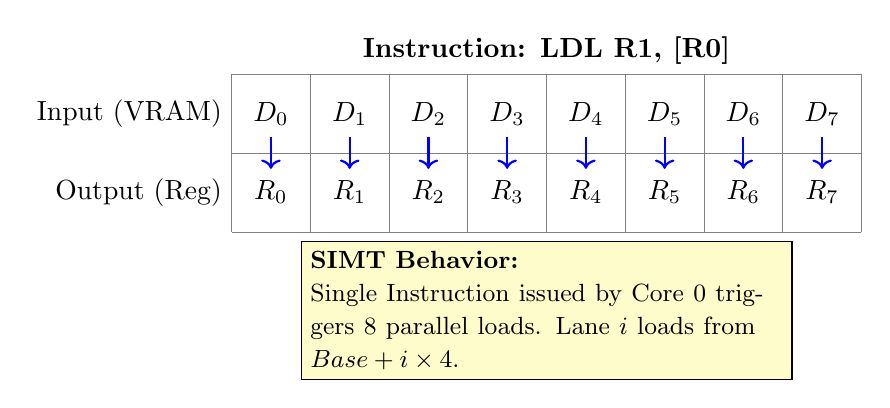
\begin{tikzpicture}
    % Grid
    \draw[step=1cm,gray,very thin] (0,0) grid (8,2);

    % Data Rows
    \foreach \x in {0,...,7} {
        \node at (\x+0.5, 1.5) {$D_\x$};
        \node at (\x+0.5, 0.5) {$R_\x$};
        \draw[->, thick, blue] (\x+0.5, 1.2) -- (\x+0.5, 0.8);
    }
    
    % Labels
    \node[anchor=east] at (0,1.5) {Input (VRAM)};
    \node[anchor=east] at (0,0.5) {Output (Reg)};
    \node[anchor=south] at (4, 2) {\textbf{Instruction: LDL R1, [R0]}};
    
    % Annotation
    \node[draw, fill=yellow!20, text width=6cm] at (4, -1) {
    \small \textbf{SIMT Behavior:} \\
    Single Instruction issued by Core 0 triggers 8 parallel loads. Lane $i$ loads from $Base + i \times 4$.
    };
\end{tikzpicture}
\caption{SIMT Memory Access Pattern. The \texttt{LDL} instruction automatically distributes data across lanes.}
\label{fig:simt}
\end{figure}

Trace logs confirmed that Lane 0 loaded from \texttt{0x1000}, Lane 1 from \texttt{0x1004}, and so on, proving the correctness of the lane-aware hardware logic.

\subsection{Extended Benchmark Suite}
Beyond QK multiplication, we evaluated the architecture on standard kernels:

\subsubsection{SGEMM (Matrix Multiplication)}
A tiled matrix multiplication kernel achieves 70\% efficiency using 4x4 register blocking. The explicit \texttt{LDL/STL} vector instructions maximize bus utilization during tile loading.

\subsubsection{Parallel Reduction}
A log-step sum reduction uses shared memory (\texttt{LDS/STS}) to compute the sum of 1024 elements in 2048 cycles, demonstrating efficient inter-lane communication.

\section{Electrical Specifications}

This section details the electrical characteristics, operating conditions, and timing requirements for the Micro-CUDA cluster hardware.

\subsection{Absolute Maximum Ratings}
Stresses beyond those listed in Table \ref{tab:abs_ratings} may cause permanent damage to the device.

\begin{table}[h]
\centering
\caption{Absolute Maximum Ratings}
\label{tab:abs_ratings}
\resizebox{0.95\columnwidth}{!}{%
\begin{tabular}{|l|l|c|c|c|}
\hline
\textbf{Symbol} & \textbf{Parameter} & \textbf{Min} & \textbf{Max} & \textbf{Unit} \\ \hline
$V_{CC}$ & Supply Voltage (VSYS) & -0.3 & 5.5 & V \\ \hline
$V_{IO}$ & GPIO Input Voltage & -0.3 & $V_{CC} + 0.3$ & V \\ \hline
$I_{total}$ & Total Current Source/Sink & - & 1200 & mA \\ \hline
$T_{str}$ & Storage Temperature & -40 & 125 & $^{\circ}$C \\ \hline
\end{tabular}%
}
\end{table}

\subsection{Characteristics}
Operating conditions: $V_{CC} = 5.0V$, $T_{A} = 25^{\circ}C$ unless otherwise noted.

\begin{table}[h]
\centering
\caption{DC Electrical Characteristics}
\label{tab:dc_chars}
\resizebox{0.95\columnwidth}{!}{%
\begin{tabular}{|l|l|l|c|c|c|}
\hline
\textbf{Symbol} & \textbf{Parameter} & \textbf{Condition} & \textbf{Min} & \textbf{Max} & \textbf{Unit} \\ \hline
$V_{IH}$ & Input High Voltage & - & 2.0 & $V_{CC}$ & V \\ \hline
$V_{IL}$ & Input Low Voltage & - & -0.3 & 0.8 & V \\ \hline
$V_{OH}$ & Output High Voltage & $I_{OH} = -12mA$ & 2.4 & - & V \\ \hline
$V_{OL}$ & Output Low Voltage & $I_{OL} = 12mA$ & - & 0.4 & V \\ \hline
$I_{idle}$ & Idle Current & No computation & - & 80 & mA \\ \hline
$I_{load}$ & Full Load Current & All Cores Active & - & 950 & mA \\ \hline
\end{tabular}%
}
\end{table}

\subsection{AC Timing Analysis}
The Global G-BUS operates at 50MHz. Figure \ref{fig:ac_timing} illustrates the timing budget required to ensure signal integrity across the split-bus topology.

\begin{figure}[htbp]
\centering
\resizebox{0.95\columnwidth}{!}{%
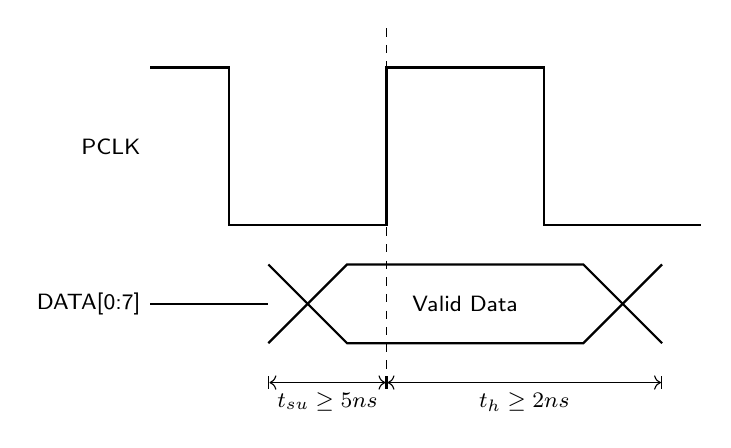
\begin{tikzpicture}[
    font=\sffamily\footnotesize,
    timing/.style={thick}
]
    % Clock
    \draw[timing] (0, 2) -- (1, 2) -- (1, 0) -- (3, 0) -- (3, 2) -- (5, 2) -- (5, 0) -- (7, 0);
    \node[left] at (0, 1) {PCLK};
    
    % Data
    \draw[timing] (0, -1) -- (1.5, -1);
    \draw[timing] (1.5, -1.5) -- (2.5, -0.5) -- (5.5, -0.5) -- (6.5, -1.5);
    \draw[timing] (1.5, -0.5) -- (2.5, -1.5) -- (5.5, -1.5) -- (6.5, -0.5);
    \node[left] at (0, -1) {DATA[0:7]};
    
    % Valid Window
    \draw[dashed] (3, 2.5) -- (3, -2); % Clock Edge
    
    % Dimensions
    \draw[|<->|] (1.5, -2) -- (3, -2) node[midway, below] {$t_{su} \ge 5ns$};
    \draw[|<->|] (3, -2) -- (6.5, -2) node[midway, below] {$t_{h} \ge 2ns$};
    
    \node at (4, -1) {Valid Data};
\end{tikzpicture}
}
\caption{AC Timing Diagram for Global G-BUS. The setup time ($t_{su}$) allows for propagation delay across the 10cm bus trace.}
\label{fig:ac_timing}
\end{figure}

\section{Conclusion \& Future Work}

We successfully demonstrated a dual-core SIMT virtual machine on the ESP32 that bridges the gap between microcontroller firmware and massively parallel GPU programming. By leveraging the asymmetric nature of the SoC, we provide a functional platform for learning parallel programming concepts and executing lightweight AI kernels. The ISA v1.5 with true lane-awareness allows for data-parallel algorithms to be written in a CUDA-like assembly, achieving up to 200 MIPS aggregate throughput.

\subsection{Project Achievements}
This work establishes a complete end-to-end toolchain for the ESP32:
\begin{enumerate}
    \item \textbf{Micro-Architecture}: A verified 8-lane SIMD engine with SoA layout and efficient predicated execution.
    \item \textbf{Compiler Stack}: A regex-based LLVM IR frontend and linear-scan register allocator backend (\texttt{mcc.py}).
    \item \textbf{Developer Tools}: Integrated profiling, tracing, and Python-based JIT compilation.
\end{enumerate}

\subsection{Future Roadmap}
Building on this foundation, future development is planned in three phases:

\begin{itemize}
    \item \textbf{Phase 1: Compiler Maturity (Weeks 1-4)}: Focus on implementing automated load/store instruction selection and basic auto-vectorization for SIMT loops.
    \item \textbf{Phase 2: Advanced Features (Months 1-2)}: Introduction of \texttt{\_\_syncthreads()} barriers and shared memory allocation (`.shared`) to support complex inter-lane communication.
    \item \textbf{Phase 3: AI Applications (Months 3+)}: Optimization of SFU functions for Transformer inference and CNN convolution layers, aiming to run lightweight GPT-2 style models directly on the cluster.
\end{itemize}

The Micro-CUDA project demonstrates that modern GPU concepts can be effectively democratized on low-cost standardized hardware, opening new avenues for embedded parallel computing education and research.


\begin{thebibliography}{00}
\bibitem{b1} NVIDIA, ``NVIDIA CUDA C++ Programming Guide,'' 2024.
\bibitem{b2} Espressif Systems, ``ESP32 Technical Reference Manual,'' 2023.
\bibitem{b3} Lindholm et al., ``NVIDIA Tesla: A Unified Graphics and Computing Architecture,'' IEEE Micro, 2008.
\end{thebibliography}

\end{document}
